% !TeX root = ./handout.tex

% things we need for forall x: YYC
\usepackage{../sty/forallxyyc}

\usepackage{lectures}

% truth values
\def\True{\ensuremath{\mathbf{\color{green!50!black}T}}}
\def\False{\ensuremath{\mathbf{\color{blue!50!black}F}}}

% input jslectureplanner metadata

\def\coursenumber{24.118}
\def\coursesection{Lec 01}
\def\coursename{Paradox \& Infinity}
\def\department{Department of Linguistics \& Philosophy}
\def\school{MIT}
\def\room{32-155}
\def\instructor{Josh Hunt}
\def\term{Spring}
\def\year{2023}
\def\shortterm{S23}

\def\deptlogo{%

\includegraphics[height=1.5cm]{../assets/logo-MIT}}

%\input{units}

%\hypersetup{pdftitle={\inserttitle\ (\insertdate)},
%pdfauthor={\insertauthor}}

% whichlecture.tex might contain \includeonlylecture etc.
\IfFileExists{whichlecture}{\input{whichlecture}}{}

\titlegraphic{%
\includegraphics[height=1.5cm]{../assets/uc-philosophy-lockup-white}}

\begin{document}
 
\newhourlecture
\newonlinelecture

{\usebackgroundtemplate{\includegraphics[width=\paperwidth]{../assets/forallx-beamer-background.pdf}}\maketitle}

\note[itemize]{
  \item Land acknowledgment
  \item Ask some hands up/down questions: For whom is this their
  first class? Who's in CPSC? Philosophy? Linguistics? Math? Who's not
  from Calgary?
  \item Experiment:
    \begin{itemize}
    \item I'll ask two questions. Don't put your hand down after the
    first question until I've asked the second.
    \item Q1 Who likes skiing or hiking?
    \item Q2 Who likes both skiing and hiking?
    \item Note if any hands went \emph{up}.
    \end{itemize}
}

\input{courseinfo}

%\setcounter{lecunit}{0}
\newonlinelecture

\section{What is logic?}
\subsection{Arguments and validity}

\begin{frame}
  \frametitle{An easy puzzle}

  \begin{block}{Where does Sanjiv live?}
  Sanjiv lives in Calgary or in Edmonton.\\
  Sanjiv doesn't live in Edmonton.
  \end{block}

  \begin{itemize}
    \item<2>[A:] Obviously, in Calgary.
  \end{itemize}

\end{frame}

\begin{frame}
  \frametitle{Arguments and sentences}

  \begin{block}{Argument 1}
  Sanjiv lives in Calgary or in Edmonton.\\
  Sanjiv doesn't live in Edmonton.\\
  Therefore, Sanjiv lives in Calgary.
  \end{block}

  \begin{itemize}[<+->]
  \item Such an argument consists of \emph{sentences}.
  \item Individual sentences are the kinds that can be \emph{true} or \emph{false}.
  \item ``Therefore'' indicates that the last sentence (supposedly)
  \emph{follows from} the first two.
  \item The last sentence is called the \emph{conclusion}.
  \item The others are called the \emph{premises}.
  \end{itemize}

\end{frame}

\begin{frame}
  \frametitle{Valid and invalid arguments}

  \begin{block}{Argument 2}
  Mandy enjoys skiing or hiking.\\
  Mandy doesn't enjoy hiking.\\
  $\therefore$ Mandy enjoys skiing.
  \end{block}

  \begin{block}{Argument 3}
  Mandy enjoys skiing or hiking.\\
  Mandy enjoys skiing.\\
  $\therefore$ Mandy doesn't enjoy hiking.
  \end{block}

  What's the difference?

  \note[itemize]{
    \begin{itemize}
    \item Arg 2 is like argument 1
    \item Think-pair-share argument 2
    \item Depending on result of experiment/agreement talk about
    inclusive/exclusive
    \item Argument 2 is valid if the ``or'' is exclusive.
    \end{itemize}
  }
\end{frame}


\begin{frame}
  \frametitle{Validity}

  \begin{definition}<1->
  A \emph{case} is some hypothetical scenario that makes each sentence
  in an argument either true or false.
  \end{definition}

  \begin{definition}<2->
  An argument is \emph{valid} if there is no case where all its
  premises are true and the conclusion is false.
  \end{definition}

  \begin{definition}<3->
  An argument is \emph{invalid} if there is at least one case where
  all its premises are true and the conclusion is false (i.e., if it
  is not valid).
  \end{definition}
\end{frame}

\begin{frame}
  \frametitle{Argument 2 is valid}

  \begin{block}{Argument 2}
  Mandy enjoys skiing or hiking.\\
  Mandy doesn't enjoy hiking.\\
  $\therefore$ Mandy enjoys skiing.
  \end{block}

Argument 2 is \emph{valid}: whenever the premises are
true, the conclusion is also true.

\end{frame}

\begin{frame}
  \frametitle{Argument 3 is not valid}

  \begin{block}{Argument 3}
  Mandy enjoys skiing or hiking.\\
  Mandy enjoys skiing.\\
  $\therefore$ Mandy doesn't enjoy hiking.
  \end{block}

  Argument 3 is \emph{invalid}: there is a possible case where the
  premises are true and the conclusion isn't (Mandy enjoys both skiing
  and hiking).

\end{frame}

\begin{frame}
  \frametitle{A harder puzzle}

  \begin{block}{Valid or invalid?}
  Sara lives in Calgary or Edmonton.\\
  Mariusz lives in Calgary unless he enjoys hiking.\\
  If Mariusz lives in Calgary, Sara doesn't.\\
  Neither Sara nor Mariusz enjoy hiking.\\
  $\therefore$ Sara lives in Edmonton.
  \end{block}

\end{frame}

\subsection{Symbolization and TFL}

\begin{frame}
  \frametitle{Validity in virtue of form}

  \begin{block}<1->{Argument 1}
  Sanjiv lives in Calgary or Edmonton.\\
  Sanjiv doesn't live in Edmonton.\\
  $\therefore$ Sanjiv lives in Calgary.
  \end{block}

  \begin{block}<1->{Argument 2}
  Mandy enjoys skiing or hiking.\\
  Mandy doesn't enjoy hiking.\\
  $\therefore$ Mandy enjoys skiing.
  \end{block}

  \begin{block}<2>{Form of arguments 1 \& 2}
  $X$ or $Y$.\\
  Not $Y$.\\
  $\therefore$ $X$.
  \end{block}

\end{frame}

\begin{frame}
  \frametitle{Some valid argument forms}

  \begin{block}{Disjunctive syllogism}
  $X$ or $Y$.\\
  Not $Y$.\\
  $\therefore\ X.$
  \end{block}

  \begin{block}{Modus ponens}
  If $X$ then $Y$.\\
  $X$.\\
  $\therefore\ Y.$
  \end{block}

  \begin{block}{Hypothetical syllogism}
  If $X$ then $Y$.\\
  If $Y$ then $Z$.\\
  $\therefore$ If $X$ then $Z$.
  \end{block}
\end{frame}

\begin{frame}
  \frametitle{Symbolizing arguments}

  \begin{block}{Symbolization key}
  $S$: Mandy enjoys skiing\\
  $H$: Mandy enjoys hiking
  \end{block}

  \begin{block}{Argument 2}
    \begin{tabular}{@{}l@{}l@{}}
      Mandy enjoys skiing or Mandy enjoys hiking.  & \ \emph{$(S \lor H)$}\\
      Not: Mandy enjoy hiking. & \emph{$\lnot H$}\\
      $\therefore$ Mandy enjoys skiing. & $\therefore$ \emph{$S$}
    \end{tabular}
  \end{block}
\end{frame}

\begin{frame}
  \frametitle{The language of TFL}

  \begin{itemize}[<+->]
  \item \emph{Sentence letters}, such as `$H$' and `$S$', to symbolize basic sentences (`Mandy likes hiking')
  \item \emph{Connectives}, to indicate how basic sentences are connected
  \begin{description}
    \item[$\lor$] either \dots or \dots
    \item[$\land$] both \dots and \dots
    \item[$\to$] if \dots then \dots
    \item[$\lnot$] not \dots
  \end{description}

  \item[] This can get complicated, e.g.:

  ``Mandy enjoys skiing or hiking, and if she lives in Edmonton, she
  doesn't enjoy both.''
  \[
  ((S \lor H) \land (E \to \lnot(S \land H)))
  \]
  \end{itemize}
\end{frame}

\subsection{What are we going to learn, and why?}

\begin{frame}
  \frametitle{What is logic?}

  \begin{itemize}[<+->]
  \item \emph{Logic is the science of what follows from what.}
  \item Sometimes a conclusion follows from the premises, sometimes it
  does not:
  \begin{itemize}[<+->]
    \item Mandy lives in Calgary.\\ Everyone who lives in Calgary likes hiking.\\
    $\therefore$ Mandy likes hiking.
    \item Mandy lives in Calgary.\\ Everyone who likes hiking lives in Calgary.\\
    $\therefore$ Mandy likes hiking.
    \end{itemize}
  \item Logic investigates what makes the first argument \emph{valid}
    and the second \emph{invalid}.
  \end{itemize}
\end{frame}

\begin{frame}
  \frametitle{What is formal logic?}

  \begin{itemize}[<+->]
  \item Studies logical properties of \emph{formal languages} (TFL and
  FOL, not English)
    \begin{itemize}[<+->]
    \item Logical consequence (what follows from what?)
    \item Logical consistency (when do sentences contradict one another?)
    \end{itemize}
  \item Expressive power (what can be expressed in a given formal
  language, and how?)
  \item Formal models (mathematical structures described by formal language)
  \item Inference and proof systems (how can it be proved that something
  follows from something else?)
  \item (Meta-logical properties of logical systems)
  \end{itemize}
\end{frame}

\begin{frame}
  \frametitle{Plan for the course}

  \begin{itemize}[<+->]
  \item Truth-functional logic (TFL)
    \begin{itemize}[<+->]
    \item Symbolization in the formal language of TFL ($H, \lor,
    \land, \to, \lnot$)
    \item Testing for validity: truth-tables
    \item Proofs in natural deduction
    \end{itemize}
  \item First-order logic (FOL)
    \begin{itemize}[<+->]
    \item More fine-grained symbolization ($E(m,h)$, $\forall$
    `every', $\exists$ `some', $=$)
    \item Semantics: interpretations
    \item Proofs in natural deduction
    \end{itemize}
  \item Some advanced topics: expressive completeness, normal forms
  \end{itemize}
\end{frame}

\begin{frame}
  \frametitle{What is logic good for? (Philosophy)}

  \begin{itemize}[<+->]
  \item Logic originates in philosophy (Aristotle), traditionally considered a sub-discipline of philosophy.
  \item Valid arguments are critical in philosophical research.
  \item Formal tools of logic are useful to make intuitive philosophical
  notions precise, e.g.,
    \begin{itemize}[<+->]
    \item Possibility and necessity
    \item Time
    \item Composition and parthood (mereology)
    \item Moral obligation and permissibility
    \item Belief and knowledge
    \end{itemize}
  \item Logic applies to semantics of natural language (philosophy of
  language, linguistics).
  \end{itemize}
\end{frame}

\begin{frame}
  \frametitle{What is logic good for? (Mathematics)}

  \begin{itemize}[<+->]
  \item Formal logic was developed in the quest for a foundations of
  mathematics (19th C.).
  \item Logical systems provide precise foundational framework for
  mathematics:
    \begin{itemize}[<+->]
    \item Axiomatic systems (e.g, geometry)
    \item Algebraic structures (e.g., groups)
    \item Set theory (e.g, Zermelo-Fraenkel with Choice)
    \end{itemize}
  \item Precision
    \begin{itemize}[<+->]
    \item Formal language makes claims more precise.
    \item Formal structures can point to alternatives, unveil gaps in proofs.
    \item Formal proof systems make proofs rigorous.
    \item Formal proofs make mechanical \emph{proof checking} and \emph{proof search} possible.
    \end{itemize}
  \end{itemize}

\end{frame}


\begin{frame}
  \frametitle{What is logic good for? (Computer Science)}

  \begin{itemize}[<+->]
    \item Computer science deals with lots of formal languages.
    \item Logic is a good example of how to set up and use formal languages.
    \item Logic : Computer Science as Calculus : Natural Science
    \item Applications of logical systems in CS are numerous:
  \begin{itemize}[<+->]
  \item Combinational logic circuits
  \item Database query languages
  \item Logic programming
  \item Knowledge representation
  \item Automated reasoning
  \item Formal specification and verification (of programs, of hardware designs)
  \item Theoretical computer science (theory of computational
  complexity, semantics of programming languages)
 \end{itemize}
\end{itemize}

\end{frame}

\newhourlecture
\newonlinelecture

\section{Symbolization in TFL}
\subsection{Symbolization keys and paraphrase}

\begin{frame}
  \frametitle{Symbolizing arguments}

  \begin{block}{Argument 2}
    Mandy enjoys skiing or Mandy enjoys hiking.\\
    Not: Mandy enjoy hiking.\\
    $\therefore$ Mandy enjoys skiing.
  \end{block}

  \begin{block}{Form of argument 2}
    $S$ or $H$.\\
    Not $H$.\\
    $\therefore$ $S$.
  \end{block}

  \begin{block}{Symbolization of argument 2 in TFL}
    $(S \lor H)$\\
    $\lnot H$\\
    $\therefore$ $S$
  \end{block}

\end{frame}

\begin{frame}
  \frametitle{Symbolization keys}

  \begin{definition}
    A symbolization key is a list that pairs \emph{sentence letters} with
    the basic English sentences they represent.
  \end{definition}

  For instance:

  \begin{block}{Symbolization key}
    $S$: Mandy enjoys skiing\\
    $H$: Mandy enjoys hiking
  \end{block}

\end{frame}

\begin{frame}
  \frametitle{Symbolization keys}

  \begin{itemize}[<+->]
  \item Sentence letters are uppercase letters, possibly with subscripts
  (e.g., $H_1$, $H_2$).
  \item Usually the symbolization key is given to you.
  \item It should not be possible to break down the ``basic
  sentences'' represented by sentence letters.

  \item[] For instance:
  \centerline{$A$: Mandy enjoys skiing or hiking}
  is bad.
  \end{itemize}
\end{frame}

\begin{frame}
  \frametitle{Paraphrase}

  \begin{itemize}[<+->]
  \item Successful symbolization sometimes requires \emph{paraphrase} to
  ensure basic sentences appear explicitly.
  \item Two things to watch for: pronouns and coordination.
  \item Pronouns stand in for singular terms (e.g., names): replace
  pronouns by those.
  \item ``or'', ``both \dots and'', ``neither \dots nor'' can connect sentences but
  also noun phrases and verb phrases: paraphrase those so they connect
  sentences.
  \end{itemize}
\end{frame}

\begin{frame}
  \frametitle{Pronouns}

  \begin{block}{Example}
    If Mandy enjoys hiking, \emph{she} also enjoys skiing.

    Replace ``she'' by ``Mandy'':\\
    If [Mandy enjoys hiking] then [Mandy enjoys skiing].
  \end{block}
\end{frame}

\begin{frame}
  \frametitle{Coordination of noun phrases}

  \begin{block}{Example}
    \emph{Mandy and Sanjiv} enjoy hiking.

    Both [Mandy enjoys hiking] and [Sanjiv enjoys hiking].
  \end{block}

  \begin{block}{Example}
    Sanjiv lives in \emph{Edmonton or Calgary}.

    Either [Sanjiv lives in Edmonton] or [Sanjiv lives in Calgary].
  \end{block}

\end{frame}

\begin{frame}
  \frametitle{Exercise caution!}

  \begin{block}{Good}
    \emph{Mandy and Sanjiv} ate pizza.

    Both [Mandy ate pizza] and [Sanjiv ate pizza].
  \end{block}

  \begin{block}{\emph{Bad}}
    \emph{Mandy and Sanjiv} ate the whole pizza.

    [Mandy ate the whole pizza] and [Sanjiv ate the whole pizza].
  \end{block}

\end{frame}

\begin{frame}
  \frametitle{Coordination of verb phrases}

  \begin{block}{Example}
  Mandy enjoys \emph{skiing or hiking}.

  Either [Mandy enjoys skiing] or [Mandy enjoys hiking].
  \end{block}

  \begin{block}{Example}
  If Sanjiv enjoys \emph{skiing and hiking}, he lives in Calgary.

  If [Sanjiv enjoys skiing] and [Sanjiv enjoys hiking], then [Sanjiv lives in Calgary].
  \end{block}

\end{frame}

\subsection{Basic symbolization}

\begin{frame}
  \frametitle{Negation}

  \begin{itemize}[<+->]
  \item \emph{Paraphrase} grammatical negation (``is not'', ``does not'') using the
  corresponding basic sentence prefixed by ``\emph{it is not the case that}.''

  \item \emph{Symbolize} ``it is not the case that $A$'' as
  \emph{$\lnot A$}.

  \begin{block}{Example}
    \begin{itemize}[<+->]
    \item[] Mandy \emph{doesn't} enjoy skiing.
    \item[] It is not the case that [\emph{Mandy enjoys skiing}].
    \item[] \emph{It is not the case that} $S$.
    \item[] $\lnot S$
    \end{itemize}
  \end{block}
  \end{itemize}
\end{frame}

\begin{frame}
  \frametitle{Conjunction}

  \begin{itemize}[<+->]
  \item \emph{Paraphrase} sentences connected by ``and'', ``but'', ``even
  though'', ``yet'', and ``although'' using
  ``\emph{both $A$ and $B$}''

  \item \emph{Symbolize} ``both $A$ and $B$'' as
  \emph{$(A \land B)$}.

  \begin{block}{Example}
  \begin{itemize}[<+->]
  \item[] \emph{Even though} Mandy lives in Edmonton\emph{,} she enjoys hiking.

  \item[] Both [\emph{Mandy lives in Edmonton}] and [\emph{Mandy enjoys hiking}].

  \item[] \emph{Both} $E$ \emph{and} $H$.

  \item[] $(E \land H)$
  \end{itemize} 
  \end{block}
\end{itemize}

\end{frame}

\begin{frame}
  \frametitle{Disjunction}

  \begin{itemize}[<+->]
  \item \emph{Paraphrase} sentences connected by ``or'' using\\
  ``\emph{either $A$ or $B$}''

  \item \emph{Symbolize} ``either $A$ or $B$'' as
  \emph{$(A \lor B)$}.

  \begin{block}{Example}
  \begin{itemize}[<+->]
  \item[] Sanjiv lives in Calgary \emph{or} Edmonton.

  \item[] Either [\emph{Sanjiv lives in Calgary}] or [\emph{Sanjiv lives in Edmonton}].

  \item[] \emph{Either} $C$ \emph{or} $E$.

  \item[] $(C \lor E)$
  \end{itemize}
  \end{block}
  
  \item[] Ignore the suggestion that ``either \dots or \dots'' is exclusive.
  We'll always treat it as inclusive unless explicitly stated.
\end{itemize}

\end{frame}

\begin{frame}
  \frametitle{Conditional}

  \begin{itemize}[<+->]
  \item \emph{Paraphrase} using ``\emph{if $A$ then $B$}'' any sentence of the form:
  \begin{itemize}[<+->]
  \item ``if $A$, $B$''
  \item ``$B$ if $A$'' (note order is reversed!)
  \item ``$B$ provided $A$''
  \end{itemize}
  \item \emph{Symbolize} ``if $A$ then $B$'' as
  \emph{$(A \eif B)$}.

  \begin{block}{Example}
  \begin{itemize}[<+->]
  \item Mandy enjoys hiking \emph{if} Sanjiv lives in Calgary.

  \item If [\emph{Sanjiv lives in Calgary}] then [\emph{Mandy enjoys hiking}].

  \item \emph{If} $C$ \emph{then} $H$.

  \item $(C \eif H)$
  \end{itemize}
  \end{block}
  \end{itemize}
\end{frame}

\begin{frame}{The parts of a conditional}

\begin{itemize}
  \item \emph{$(A \eif B)$} symbolizes:
  \begin{itemize}
    \item ``if $A$, $B$''
    \item ``$B$ if $A$'' (note order is reversed!)
    \item ``$B$ provided $A$''
  \end{itemize}
  \item $A$ is the \emph{antecedent}: it symbolizes the condition that has to
  be met for the ``then'' part to apply.
  \item $B$ is the \emph{consequent}: it symbolizes what must be true
  if the antecedent condition is true.
\end{itemize}
\end{frame}

\begin{frame}
  \frametitle{Mix \& match}

  \begin{block}{Example}
    \begin{itemize}[<+->]
      \item[] Mandy doesn't enjoy hiking, \emph{provided} Sanjiv lives in Calgary or Edmonton.

  \item[] If [Sanjiv lives in Calgary \emph{or} Edmonton] then [Mandy \emph{doesn't} enjoy hiking].

  \item[] If [either [\emph{Sanjiv lives in Calgary}] or [\emph{Sanjiv lives in Edmonton}]]
  then [it is not the case that [\emph{Mandy enjoys hiking}]].

  \item[] If [either $C$ or $E$]
  then [it is not the case that $H$].

  \item[] $((C \lor E) \eif \lnot H)$
  \end{itemize}
  \end{block}

\end{frame}

\subsection{Conditionals}

\begin{frame}
  \frametitle{A logic puzzle}

\begin{itemize}
\item Every card has a letter on one side and a number on the other side.
\item You're a card inspector tasked with making sure that cards satisfy this quality standard:

\bigskip
\begin{quote}
If a card has an even number on one side, then it has a vowel on the other.
\end{quote}
\end{itemize}

\end{frame}

\frame<1>[label=wason]{
  \frametitle{A logic puzzle}

Which card(s) do you have to turn over to make sure that:
\bigskip

\begin{quote}
If a card has an even number on one side, then it has a vowel on the other.
\end{quote}

\begin{tabular}{cccc}
\begin{beamerboxesrounded}[width=5em]{}
\vskip 2ex
\hfil \Large E\hfil\\
\end{beamerboxesrounded} &
\begin{beamerboxesrounded}[width=5em]{}
\vskip 2ex
\hfil \Large \alert<2>{K}\hfil\\
\end{beamerboxesrounded} &
\begin{beamerboxesrounded}[width=5em]{}
\vskip 2ex
\hfil \Large 3\hfil\\
\end{beamerboxesrounded} &
\begin{beamerboxesrounded}[width=5em]{}
\vskip 2ex
\hfil \Large \alert<2>{4}\hfil\\
\end{beamerboxesrounded} \\
(1) & \alert<2>{(2)} & (3) & \alert<2>{(4)}
\end{tabular}

}

\begin{frame}
  \frametitle{Another logic puzzle}

\begin{itemize}
\item At an all-ages event where everyone has a drink
\item You know how old some of the people are, and you can tell what some of them are drinking
\item You're tasked with making sure that the following rule is followed:
\bigskip 

\begin{quote}
If a person is drinking alcohol, then they are at least 18 years old.
\end{quote}
\end{itemize}

\end{frame}

\begin{frame}
  \frametitle{Another logic puzzle}

Which of these people do you have to check (age or drink) to ensure
that:
\bigskip

\begin{quote}
If a person is drinking alcohol, then they must be at least 18 years old.
\end{quote}

\begin{tabular}{cccc}
\begin{beamerboxesrounded}[width=5em]{}
\vskip 2ex
\Large 22 years\\
\end{beamerboxesrounded} &
\begin{beamerboxesrounded}[width=5em]{}
\vskip 2ex
\Large \alert<2>{16 years}\\
\end{beamerboxesrounded} &
\begin{beamerboxesrounded}[width=5em]{}
\vskip 2ex
\Large drinks pop\\
\end{beamerboxesrounded} &
\begin{beamerboxesrounded}[width=5em]{}
\vskip 2ex
\Large \alert<2>{drinks beer}\\
\end{beamerboxesrounded} \\
(1) & \alert<2>{(2)} & (3) & \alert<2>{(4)}
\end{tabular}

\end{frame}

\againframe<2|handout:0>{wason}

\begin{frame}
  \frametitle{Truth conditions of conditionals}

\[\text{If\ } \underbrace{\text{X is drinking alcohol}}_{A},
\text{then\ }\underbrace{\text{X is over 18}}_{B}\]

\begin{itemize}[<+->]
\item ``If $A$, then $B$'' can only be \emph{false} if:
\begin{itemize}
\item $A$ is \emph{true}: we check age if X is drinking beer ($A$~true), not if
 drinking pop; \emph{and}
\item $B$ is \emph{false}: we check drink if X underage ($B$ false),\\ not
if over 18 ($B$ true)
\end{itemize}
\item ``If $A$, then $B$'' is true if:
\begin{itemize}
\item $A$ is \emph{false} (we don't check people drinking pop); \emph{or}
\item $B$ is \emph{true} (we don't card if X is over 18);
\item (or both)
\end{itemize}
\end{itemize}
\end{frame}


\subsection{``Only if'' and ``unless''}

\begin{frame}
  \frametitle{`If' and `only if'}

\begin{itemize}[<+->]
  \item Sue drinks beer ($A$) \emph{only if} she is over 18 ($B$)
  \[
  A \eif B
  \]
  \item False if Sue is underage, but drinks beer.
  \item Sue drinks beer ($A$) if she is over 18 ($B$).
  \[
  B \eif A
  \]
  \item False if she's 25 but drinks pop.
  \item Not false if she's 16 and drinking beer.
\end{itemize}
\end{frame}

\begin{frame}
  \frametitle{Conditional}

  \begin{itemize}[<+->]
  \item \emph{Paraphrase} ``$A$ only if $B$'' as
  ``\emph{if $A$ then $B$}''.
  \item \emph{Symbolize} ``$A$ only if $B$'' as
  \emph{$(A \eif B)$}.
  \item Note: 
    \begin{itemize} \item ``$A$ if $B$'' is $(B \eif A$)\\
  \item ``$A$ only if $B$'' is $(A \eif B$)
    \end{itemize}
  \item \emph{Symbolize} ``$A$ if and only if $B$'' as
  \emph{$(A \eiff B)$}.
\end{itemize}
\end{frame}

\begin{frame}
\frametitle{Unless}

Which of these people do you have to check (age or drink) to ensure that:
\begin{quote}
People are drinking pop unless they are over 18.
\end{quote}

\begin{tabular}{cccc}
\begin{beamerboxesrounded}[width=5em]{}
\vskip 2ex
\Large 22 years\\
\end{beamerboxesrounded} &
\begin{beamerboxesrounded}[width=5em]{}
\vskip 2ex
\Large 16 years\\
\end{beamerboxesrounded} &
\begin{beamerboxesrounded}[width=5em]{}
\vskip 2ex
\Large drinks pop\\
\end{beamerboxesrounded} &
\begin{beamerboxesrounded}[width=5em]{}
\vskip 2ex
\Large drinks beer\\
\end{beamerboxesrounded} \\
(1) & (2) & (3) & (4)
\end{tabular}

\end{frame}


\begin{frame}
\frametitle{Unless}

\[\underbrace{\text{X is drinking pop}}_{A},
\text{unless\ }\underbrace{\text{X is over 18}}_{B}\]

\begin{itemize}[<+->]
\item ``$A$ unless $B$'' can only be \emph{false} if:
\begin{itemize}
\item $A$ is \emph{false}\\
(we check age if person is drinking beer), \emph{and}
\item $B$ is \emph{false}\\
(we check drink if person not at least 18)
\end{itemize}
\item ``$A$ unless $B$'' is true (test OK) if
$A$ or $B$ or both are true.
\item ``$A$ unless $B$'' can be paraphrased and symbolized by:
\begin{itemize}
\item ``$A$ if not $B$'' ($\enot B \eif A$)
\item ``either $A$ or $B$'' ($A \eor B$)
\end{itemize}
\end{itemize}

\end{frame}

\begin{frame}
  \frametitle{Unless}

  Treat ``\emph{unless}'' the same way you would treat ``or''

  \begin{block}{Example}
  Mandy enjoys hiking unless Sanjiv lives in Calgary.

  $(H \eor C)$
  \end{block}
\end{frame}


\subsection{More connectives}

\begin{frame}
  \frametitle{If and only if}

  \begin{block}{Example}
    \begin{itemize}[<+->]
    \item[] Mandy enjoys hiking if and only if she enjoys skiing.
    \item[] Both [if $S$ then $H$] and [if $H$ then $S$].
    \item[] $((S \eif H)\eand(H \eif S))$
    \item[] $(H \eiff S)$
    \end{itemize}
  \end{block}

\end{frame}

\begin{frame}
  \frametitle{Exclusive or}

  \uncover<7->{\emph{Paraphrase} sentences containing ``either $A$ or $B$ but not both'' using\\
  ``\emph{both [either $A$ or $B$] and\\ \qquad [it is not the case
  that [both $A$ and $B$]]}''}

  \begin{block}{Example}
  Mandy enjoys \alert<1>{hiking or skiing} \alert<5>{but} \alert<3>{not both}.

  \uncover<6->{Both} \uncover<2->{[either $H$ or $S$]} \uncover<6->{and}\\ \phantom{Both} \uncover<4->{[it is not the case that [both
  $H$
  and $S$]].}

  \uncover<8>{$((H \eor S) \land \lnot(H \eand S))$}
  \end{block}

\end{frame}

\begin{frame}
  \frametitle{Neither \dots nor \dots}

  \uncover<2->{\emph{Paraphrase} sentences containing ``neither $A$ nor $B$'' using\\
  ``\emph{both [it is not the case that $A$] and\\ \qquad [it is not the case
  that $B$]}''}

  \begin{block}{Example}
  Mandy enjoys neither hiking nor skiing.

  \uncover<2->{Both [it is not the case that $H$] and\\ \qquad [it is not the case that $S$].}

  \uncover<3>{$(\lnot H \land \lnot S)$}
  \end{block}

\end{frame}

\begin{frame}
  \frametitle{Mix \& match}
  \begin{block}{Example}
  Sara lives in Calgary or Edmonton.\\
  \uncover<2->{\emph{Either [Sara lives in Calgary] or [Sara lives in Edmonton].}}\\
  Mariusz lives in Calgary unless he enjoys hiking.\\
  \uncover<3->{\emph{Either [Mariusz lives in Calgary] or [Mariusz
    enjoys hiking].}}\\
  If Mariusz lives in Calgary, Sara doesn't.\\
  \uncover<4->{\emph{If [Mariusz lives in Calgary] then [it is not
    the case that [Sara lives in Calgary]].}}\\
  Neither Sara nor Mariusz enjoy hiking.\\
  \uncover<5->{\emph{Both [it is not the case that [Sara enjoys
      hiking]] and [it is not the case that [Mariusz enjoys hiking]].}}\\
  $\therefore$ Sara lives in Edmonton.
  \end{block}
\end{frame}

\begin{frame}
  \frametitle{Mix \& match}

  \begin{block}{Example}
  Sara lives in Calgary or Edmonton.\\
  \alert{$(C \eor E)$}\\
  Mariusz lives in Calgary unless he enjoys hiking.\\
  \alert{$(A \eor M)$}\\
  If Mariusz lives in Calgary, Sara doesn't.\\
  \alert{$(A \eif \enot C)$}\\
  Neither Sara nor Mariusz enjoy hiking.\\
  \alert{$( \enot S \eand\enot M)$}\\
  $\therefore$ Sara lives in Edmonton.\\
  \alert{$\therefore\ E$}.
  \end{block}
\end{frame}

\subsection{Ambiguity}

\begin{frame}
    \frametitle{Types of ambiguity}

\begin{itemize}
  \item Lexical ambiguity: one word---many meanings \\
  e.g., ``bank'', ``crane''
  \item Syntactic ambiguity: one sentence---many readings\\
  e.g.,
  \begin{itemize}
  \item ``Flying planes can be dangerous'' (Chomsky)
  \item ``One morning I shot an elephant in my pajamas.\\ How he got in my pajamas, I don't know.'' (Groucho Marx)
  \end{itemize}
\end{itemize}

\end{frame}

\begin{frame}
  \frametitle{The man who was hanged by a comma}

\begin{columns}
\begin{column}{3cm}
\pgfimage[width=3cm]{../assets/casement}
\end{column}
\begin{column}{7cm}
\begin{itemize}
\item Sir Roger Casement (1864--1916)
\item British consul to Congo and Peru
\item Tried to recruit Irish revolutionaries in Germany during WWI
\item Tried for treason
\end{itemize}
\end{column}
\end{columns}

\end{frame}

\begin{frame}
  \frametitle{Treason Act of 1351}

\small
ITEM, Whereas divers Opinions have been before this Time in what Case
Treason shall be said, and in what not; the King, at the Request of
the Lords and of the Commons, hath made a Declaration in the Manner as
hereafter followeth, that is to say; When a Man doth compass or
imagine the Death of our Lord the King, or of our Lady his Queen or of
their eldest Son and Heir; or if a Man do violate the King's
Companion, or the King's eldest Daughter unmarried, or the Wife of the
King's eldest Son and Heir; or \emph{if a Man} do levy War against our Lord
the King in his Realm, or \emph{be adherent to the King's Enemies in his
Realm, giving to them Aid and Comfort in the Realm}\onslide<2>{\colorbox{highlightbg}{\textbf{,}}} \emph{or elsewhere}, and
thereof be probably attainted of open Deed by the People of their
Condition: \dots And it is to be
understood, that in the Cases above rehearsed, that ought to be judged
Treason which extends to our Lord the King, and his Royal Majesty:
\dots

\end{frame}

\begin{frame}
  \frametitle{R v. Casement in FOL}
  \begin{itemize}[<+->]
\item Symbolization key:
  \begin{ekey}
    \item[A] Casement was adherent to the King's enemies in the realm.
    \item[G] Casement gave aid and comfort to the King's enemies in the realm.
    \item[B] Casement was adherent to the King's enemies abroad.
    \item[H] Casement gave aid and comfort to the King's enemies abroad.
  \end{ekey}
  \item Not treason:
  \begin{earg}
    \item[] $A \lor (G \lor H)$
  \end{earg} \item Treason:
  \begin{earg}
    \item[] $(A \lor B) \lor (G \lor H)$
  \end{earg}
\end{itemize}
\end{frame}

\begin{frame}
  \frametitle{Ambiguity of \eand{} and \eor}

  \begin{itemize}[<+->]
    \item English sentences don't have parentheses.
    \item This can lead to ambiguity, e.g.,
    \begin{earg}
      \item[] Ahmed admires Brit and Cara or Dina.
    \end{earg}
    \item It might mean one of:
    \begin{earg}
      \item[] Ahmed admires either [both Brit and Cara] or Dina.
      \item[] Ahmed admires both Brit and [either Cara or Dina].
    \end{earg}
    \item In TFL, symbolizations are unambiguous:
    \begin{earg}
      \item[] $((B \eand C) \eor D)$
      \item[] $(B \eand (C \eor D))$
    \end{earg}
  \end{itemize}
\end{frame}


\newhourlecture
\newonlinelecture

\section{TFL and truth tables}

\subsection{Characteristic truth tables}

\begin{frame}
\frametitle{Sentence letters and connectives}

  \begin{itemize}[<+->]
    \item Symbolization involves \emph{sentence letters} like $H$ and
    \emph{connectives} ($\enot$, $\eor$, $\eand$, $\eif$, $\eiff$)
    \item Recall that a \emph{case} makes basic sentences \emph{true}
    or \emph{false} (and never both).
    \item So if we can determine \emph{truth conditions} for sentences
   involving connectives, we can assign \emph{true} and \emph{false}
   also to results of symbolization.
    \item[]
  \begin{block}{When is $(H \eand S)$ true?}
    \begin{itemize}[<+->]
      \item[] $(H \eand S)$ is true if and only if $H$ is true and $S$ is also
  true.

  \item[] Suppose a case makes $H$ true and $S$ false.

  \item[] In that case, $(H \eand S)$ would be \only<8|handout:0>{???}\only<9>{\emph{false}}.
\end{itemize} 
\end{block}
\end{itemize}
\end{frame}

\begin{frame}
  \frametitle{Negation \enot}

  \begin{definition}
  $\enot \metav A$ is true iff $\metav A$ is false.
  \end{definition}

  Characteristic truth table:
  \begin{center}
  \begin{tabular}{c|c}
  \metav{A} & \enot\metav{A}\\
  \hline
  \True & \False\\
  \False & \True
  \end{tabular}
  \end{center}
\end{frame}

\begin{frame}
  \frametitle{Conjunction \eand}

  \begin{definition}
  $(\metav A \eand \metav B)$ is true iff $\metav A$ is true and
  $\metav B$ is true, and false otherwise.
  \end{definition}

  Characteristic truth table:
  \begin{center}
  \begin{tabular}{c c |c}
  \metav{A} & \metav{B} & $(\metav{A}\eand\metav{B})$\\
  \hline
  \True & \True & \True\\
  \True & \False & \False\\
  \False & \True & \False\\
  \False & \False & \False
  \end{tabular}
  \end{center}
\end{frame}

\begin{frame}
  \frametitle{Disjunction \eor}

  \begin{definition}
  $(\metav A \eor \metav B)$ is true iff $\metav A$ is true or
  $\metav B$ is true (or both), and false otherwise.
  \end{definition}

  Characteristic truth table:
  \begin{center}
  \begin{tabular}{c c |c}
  \metav{A} & \metav{B} & $(\metav{A}\eor\metav{B})$\\
  \hline
  \True & \True & \True\\
  \True & \False & \True\\
  \False & \True & \True\\
  \False & \False & \False
  \end{tabular}
  \end{center}
\end{frame}

\againframe<2>{wason}

\begin{frame}
\frametitle{The material conditional \eif}

\begin{definition}
  $(\metav A \eif \metav B)$ is true iff $\metav A$ is false or
  $\metav B$ is true (or both), and false otherwise.
  \end{definition}
\[
\begin{array}{cc|c}
\metav{A} & \metav{B} & (\metav{A} \eif \metav{B})\\
\hline
\True & \True & \True\\
\True & \False & \False\\
\False & \True & \True\\
\False & \False & \True
\end{array}
\]
\end{frame}

\begin{frame}
  \frametitle{The material biconditional \eiff}
  
  \begin{definition}
    $(\metav A \eiff \metav B)$ is true iff $\metav A$ and
    $\metav B$ have the same truth value, and false otherwise.
    \end{definition}
  \[
  \begin{array}{cc|c}
  \metav{A} & \metav{B} & (\metav{A} \eiff \metav{B})\\
  \hline
  \True & \True & \True\\
  \True & \False & \False\\
  \False & \True & \False\\
  \False & \False & \True
  \end{array}
  \]
  
\end{frame}

\subsection{Sentences of TFL}

\begin{frame}
\frametitle{Sentences of TFL}

  \begin{definition}
  \begin{enumerate}
  \item Every sentence letter is a sentence.
  \item If $\metav{A}$ is a sentence, then $\enot\metav{A}$ is a sentence.
  \item If $\metav{A}$ and $\metav{B}$ are sentences, then
  \begin{itemize}
  \item $(\metav{A}\eand\metav{B})$ is a sentence.
  \item $(\metav{A}\eor\metav{B})$ is a sentence.
  \item $(\metav{A}\eif\metav{B})$ is a sentence.
  \item $(\metav{A}\eiff\metav{B})$ is a sentence.
  \end{itemize}
  \item Nothing else is a sentence.
  \end{enumerate}
  \end{definition}

  The indicated connective is called the \emph{main connective}.
\end{frame}

\begin{frame}
  \frametitle{Construction of sentences}

  \begin{itemize}[<+->]
    \item $H$ is a sentence.
    \item $S$ is a sentence.
    \item $(H \mathbin{\emph{\eor}} S)$ is a sentence.
    \item $(H \mathbin{\emph{\eand}} S)$ is a sentence.
    \item $\emph{\enot} (H \eand S)$ is a sentence.
    \item $((H \eor S) \mathbin{\emph{\eand}} \enot (H \eand S))$ is a sentence.
  \end{itemize}

\uncover<7>{(Main connective is \emph{highlighted}.)}

\end{frame}

\begin{frame}
  \frametitle{Examples of non-sentences}

  \begin{itemize}
    \item $\mathit{HikesMandy}$\\
    \qquad single sentence letters
    \item $(H \mathbin{\enot} S)$\\
    \qquad$\enot$ can't go between sentences
    \item $(H \eand S \eand C)$\\
    \qquad $\eand$ combines only two sentences
    \item $(\enot H)$\\
    \qquad no parentheses around $\enot H$
    \item $(H \eif (S \eand C)$\\
    \qquad missing closing parenthesis
    \item $H \eor S$\\
    \qquad missing parentheses
    \item $[H \eif (S \eand C)]$\\
    \qquad only one kind of parentheses
  \end{itemize}

\end{frame}

\subsection{Valuations}

\begin{frame}
  \frametitle{Valuations}

  \begin{definition}
  A \emph{valuation} is an assignment of \emph{\True} or \emph{\False} to each
  sentence letter in a sentence or sentences.
  \end{definition}

  \begin{definition}
  The \emph{truth value of a sentence} \metav{S} on a valuation is:
  \begin{enumerate}
  \item if \metav{S} is a sentence letter: the truth value assigned to
  it
  \item if \metav{S} is $\enot \metav{A}$: opposite of the truth value of
  $\metav{A}$
  \item if \metav{S} is $(\metav{A} \ast \metav{B})$:
  result of characteristic truth table of~$\ast$ for truth values of
  $\metav{A}$ and $\metav{B}$.
  \end{enumerate}
  \end{definition}
\end{frame}

\begin{frame}
  \frametitle{Computing truth values}

Valuation: $H$ is \True, $S$ is \False.

On this valuation:

  \begin{itemize}
    \item $H$ is \True.
    \item $S$ is \False.
    \item $(H \eor S)$ is \True\ (because $\True \eor \False$ gives \True).
    \item $(H \eand S)$ is \False\ (because $\True \eand \False$ gives \False).
    \item $\enot (H \eand S)$ is \True\ (because $\enot \False$ is $\True$).
    \item $((H \eor S) \eand \enot (H \eand S))$ is \True\
    (because $\True \eand \True$ gives $\True$).
  \end{itemize}

\end{frame}

\begin{frame}
\frametitle{Computing truth values}

\setbeamercovered{still covered={\opaqueness<1->{0}},
again covered={\opaqueness<1->{30}}}

\begin{tabular}{c c|r c l c l r c l}
$H$ & $S$ & $(\alert<4>{(H}$ & \alert<3-4>{\eor} & $\alert<4>{S)}$ & \alert<9>{\eand} & $\alert<7-8>{\enot}$ & $\alert<6,8>{(H}$ & \alert<5-6,8>{\eand} & $\alert<6,8>{S)})$\\
\hline
 \True & \False &
 \uncover<2-4>{\alert<3>{\True}} &
 \uncover<4,9->{\alert<4,9>{\True}} &
 \uncover<2-4>{\alert<3>{\False}} &
 \uncover<10->{\alert<10>{\True}} &
 \uncover<8-10>{\alert<8-9>{\True}} &
 \uncover<2,5-6>{\alert<5>{\True}} &
 \uncover<6-8>{\alert<6-7>{\False}} &
 \uncover<2,5-6>{\alert<5>{\False}}\\
 & & & \only<3-4|handout:0>{$\uparrow$} & & \only<9-10>{$\uparrow$} &
 \only<7-8|handout:0>{$\uparrow$} & & \only<5-6|handout:0>{$\uparrow$}
\end{tabular}
\begin{itemize}
  \item<2-> Copy truth values under sentence letters.
  \item<3-> Compute values of parts that combine sentence letters.
  \item<7-> Use computed values for larger parts.
  \item<10-> Done when you have the value under the main connective.
\end{itemize}
\end{frame}

\subsection{Validity and truth tables}

\begin{frame}
  \frametitle{Validity}

  \begin{itemize}[<+->]
  \item In English: an argument is \emph{valid} if there is no \emph{case}
  where all premises are true and conclusion is false.

  \item A \emph{case} must make every \emph{basic sentence} true or false
  (and not both).

  \item In TFL, \emph{valuations} make every \emph{sentence letter} true or
  false (and not both).

  \item Also: every valuation makes every \emph{sentence} true or false (and
  not both), and we can compute the truth value.
  \end{itemize}
\end{frame}

\begin{frame}
  \frametitle{Validity in TFL}

  \begin{definition}
  An argument is \emph{valid in TFL} if there is \emph{no} valuation in which
  all premises are \True{} and the conclusion is \False.

  An argument is \emph{invalid in TFL} if there is \emph{at least one}
  valuation in which all premises are \True{} and the conclusion is
  \False.
  \end{definition}
\end{frame}

\begin{frame}
  \frametitle{Disjunctive syllogism}

\setbeamercovered{still covered={\opaqueness<1->{0}},
again covered={\opaqueness<1->{30}}}

  \begin{columns}[c]
  \begin{column}{2cm}
  \begin{earg}
  \item[] $H \eor S$
  \item[] $\enot S$
  \item[\therefore] $H$
  \end{earg}
  \end{column}
  \begin{column}{5cm}
  \[\begin{array}{cc|rcl|rc|cc}
  H & S & (H & \eor & S) & \enot & S & H & \phantom{\leftarrow}\\
  \hline
    \uncover<2->{\alert<2>{\True}} &
    \uncover<2->{\alert<2>{\True}} &
    \uncover<3-4>{\True} &
    \uncover<4,8->{\alert<4>{\True}} &
    \uncover<3-4>{\True} &
    \uncover<6,8->{\alert<6,9>{\False}} &
    \uncover<5-6>{\True} &
    \uncover<7->{\True} &
    \only<9|handout:0>{\leftarrow}\only<10->{\checkmark}
    \\
    \uncover<2->{\alert<2>{\True}} &
    \uncover<2->{\alert<2>{\False}} &
    \uncover<3-4>{\True} &
    \uncover<4,8->{\alert<4>{\True}} &
    \uncover<3-4>{\False} &
    \uncover<6,8->{\alert<6>{\True}} &
    \uncover<5-6>{\False} &
    \uncover<7->{\alert<10>{\True}} &
    \only<10|handout:0>{\leftarrow}\only<11->{\checkmark}
    \\
    \uncover<2->{\alert<2>{\False}} &
    \uncover<2->{\alert<2>{\True}} &
    \uncover<3-4>{\False} &
    \uncover<4,8->{\alert<4>{\True}} &
    \uncover<3-4>{\True} &
    \uncover<6,8->{\alert<6,11>{\False}} &
    \uncover<5-6>{\True} &
    \uncover<7->{\False} &
    \only<11|handout:0>{\leftarrow}\only<12->{\checkmark}
  \\
    \uncover<2->{\alert<2>{\False}} &
    \uncover<2->{\alert<2>{\False}} &
    \uncover<3-4>{\False} &
    \uncover<4,8->{\alert<4,12>{\False}} &
    \uncover<3-4>{\False} &
    \uncover<6,8->{\alert<6>{\True}} &
    \uncover<5-6>{\False} &
    \uncover<7->{\False} &
    \only<12|handout:0>{\leftarrow}\only<13->{\checkmark}
  \end{array}\]
  \end{column}
  \end{columns}
  \begin{itemize}
  \item \alert<2|handout:0>{List all valuations for $H$, $S$.}
  \item \alert<3-7|handout:0>{Compute truth values of premises, conclusion.}
  \item \alert<8-12|handout:0>{Check each valuation: one premise \False, or conclusion \True?}
  \item \alert<13|handout:0>{All valuations check out: valid.}
  \end{itemize}
\end{frame}

\begin{frame}
  \frametitle{An invalid argument}

\setbeamercovered{still covered={\opaqueness<1->{0}},
again covered={\opaqueness<1->{30}}}

  \begin{columns}[c]
  \begin{column}{2cm}
  \begin{earg}
  \item[] $H \eor S$
  \item[] $H$
  \item[\therefore] $\enot S$
  \end{earg}
  \end{column}
  \begin{column}{5cm}
  \[\begin{array}{cc|rcl|r|ccc}
  H & S & (H & \eor & S) &  H & \enot & S & \phantom{\leftarrow}\\
  \hline
    \uncover<2->{\alert<2>{\True}} &
    \uncover<2->{\alert<2>{\True}} &
    \uncover<3>{\True} &
    \uncover<3->{\alert<3,6>{\True}} &
    \uncover<3>{\True} &
    \uncover<3->{\alert<3,6>{\True}} &
    \uncover<3->{\alert<3,6>{\False}} &
    \uncover<3>{\True} &
    \only<5|handout:0>{\leftarrow}\only<6->{\alert{\text{\ding{55}}}}
    \\
    \uncover<2->{\alert<2>{\True}} &
    \uncover<2->{\alert<2>{\False}} &
    \uncover<3>{\True} &
    \uncover<3->{\alert<3>{\True}} &
    \uncover<3>{\False} &
    \uncover<3->{\alert<3>{\True}} &
    \uncover<3->{\alert<3,7>{\True}} &
    \uncover<3>{\False} &
    \only<7|handout:0>{\leftarrow}\only<8->{\checkmark}
    \\
    \uncover<2->{\alert<2>{\False}} &
    \uncover<2->{\alert<2>{\True}} &
    \uncover<3>{\False} &
    \uncover<3->{\alert<3>{\True}} &
    \uncover<3>{\True} &
    \uncover<3->{\alert<3,8>{\False}} &
    \uncover<3->{\alert<3>{\False}} &
    \uncover<3>{\True} &
    \only<8|handout:0>{\leftarrow}\only<9->{\checkmark}
  \\
    \uncover<2->{\alert<2>{\False}} &
    \uncover<2->{\alert<2>{\False}} &
    \uncover<3>{\False} &
    \uncover<3->{\alert<3,9>{\False}} &
    \uncover<3>{\False} &
    \uncover<3->{\alert<3,9>{\False}} &
    \uncover<3->{\alert<3>{\True}} &
    \uncover<3>{\False} &
    \only<9|handout:0>{\leftarrow}\only<10->{\checkmark}
  \end{array}\]
  \end{column}
  \end{columns}
  \begin{itemize}
  \item \alert<2|handout:0>{List all valuations for $H$, $S$.}
  \item \alert<3-4|handout:0>{Compute truth values of premises, conclusion.}
  \item \alert<5|handout:0>{Check each valuation: one premise \False, or conclusion \True?}
  \item \alert<6|handout:0>{Find a valuation with all premises \True{} and conclusion \False: invalid.}
  \end{itemize}
\end{frame}


\newhourlecture



\subsection{Large truth tables}


\begin{frame}
\frametitle{Large truth tables}

\begin{itemize}[<+->]
\item For arguments with $n$ sentence letters, there are $2^n$
possible valuations
\begin{itemize}[<+->]
\item A single letter $A$ can be \True{} or \False{}: $2^1 = 2$ valuations.
\item For two letters $A$, $B$: $B$ can be \True{} or \False{} for every
possible valuation (2) of $A$: $2 \times 2 = 2^2 = 4$ valuations
\item For three letters $A$, $B$, $C$: $C$ can be \True{} or \False{}
for every possible valuation (4) of $A$ and $B$: $2 \times 4 = 2^3 =
8$ valuations
\item Etc.
\end{itemize}
\item In the $i$th reference column, alternate \True{} and \False{}
every $2^{n-i}$ lines
\end{itemize}
\end{frame}


\begin{frame}
  \frametitle{A complex truth table}
  
  3 sentence letters $A$, $C$, $E$: $2^3 = 8$ lines
  \footnotesize
    \[\begin{array}{lccc|c}
    & A & C & E & \dots\\
     \cline{2-5}
    1 & \uncover<3->{\True} & \uncover<4->{\True} &
     \uncover<5->{\True} & \dots \\
    2 & \uncover<3->{\True} & \uncover<4->{\True} &
     \uncover<5->{\False} & \dots \\
    3 & \uncover<3->{\True} & \uncover<4->{\False} &
     \uncover<5->{\True} & \dots \\
    4 & \uncover<3->{\True} & \uncover<4->{\False} &
     \uncover<5->{\False} & \dots \\
    5 & \uncover<3->{\False} & \uncover<4->{\True} &
    \uncover<5->{\True} & \dots \\
    6 & \uncover<3->{\False} & \uncover<4->{\True} &
    \uncover<5->{\False} & \dots \\
    7 & \uncover<3->{\False} & \uncover<4->{\False} &
    \uncover<5->{\True} & \dots \\
    8 & \uncover<3->{\False} & \uncover<4->{\False} &
    \uncover<5->{\False} & \dots \\
    & \uncover<2>{\uparrow} &\uncover<3>{\uparrow} & \multicolumn{1}{c}{\uncover<4>{\uparrow}}\\
    & \multicolumn{4}{l}{\uncover<2->{\text{alternate every \dots}}} \\
    & \uncover<2>{4} & \uncover<3>{2} & \multicolumn{1}{c}{\uncover<4->{1}} \\
    & \multicolumn{4}{l}{\uncover<2->{\text{rows}}} \\
    \end{array}\]
  \end{frame}
  
\begin{frame}
  \frametitle{Example (simplified)}

  Sara lives in Calgary or Edmonton.\\
  Mariusz lives in Calgary unless he enjoys hiking.\\
  If Mariusz lives in Calgary, Sara doesn't.\\
  Mariusz doesn't enjoy hiking.\\
  $\therefore$ Sara lives in Edmonton.

  \begin{align*}
  & C \eor E\\
  & A \eor M\\
  & A \eif \enot C\\
  &\enot M\\
  \therefore & E
  \end{align*}
\end{frame}

\begin{frame}\footnotesize
\setbeamercovered{still covered={\opaqueness<1->{0}},
again covered={\opaqueness<1>{20}\opaqueness<2->{10}}}
\[
  \begin{array}{cccc|cec|cec|ceec|ef|f}
  A &  C & E & M & C &\eor & E & A & \eor & M & A & \eif & \enot & C & \enot & M & E\\
  \hline
  \True & \True & \True & \True &
    \uncover<2>{\True} & \uncover<3-4>{\True} & \uncover<2>{\True} &
    \uncover<2>{\True} & \uncover<3-4>{\True} & \uncover<2>{\True} &
    \uncover<2>{\True} & \uncover<3->{\False} & \uncover<3>{\False} & \uncover<2>{\True} &
    \uncover<3->{\False} & \uncover<2>{\True} & \uncover<2-5>{\True} \\
  \True & \True & \True & \False &
    \uncover<2>{\True} & \uncover<3-4>{\True} & \uncover<2>{\True} &
    \uncover<2>{\True} & \uncover<3-4>{\True} & \uncover<2>{\False} &
    \uncover<2>{\True} & \uncover<3->{\False} & \uncover<3>{\False} & \uncover<2>{\True} &
    \uncover<3-4>{\True} & \uncover<2>{\False} & \uncover<2-5>{\True} \\
  \True & \True & \False & \True &
    \uncover<2>{\True} & \uncover<3-4>{\True} & \uncover<2>{\False} &
    \uncover<2>{\True} & \uncover<3-4>{\True} & \uncover<2>{\True} &
    \uncover<2>{\True} & \uncover<3->{\False} & \uncover<3>{\False} & \uncover<2>{\True} &
    \uncover<3->{\False} & \uncover<2>{\True} & \uncover<2-4>{\False} \\
  \True & \True & \False & \False &
    \uncover<2>{\True} & \uncover<3-4>{\True} & \uncover<2>{\False} &
    \uncover<2>{\True} & \uncover<3-4>{\True} & \uncover<2>{\False} &
    \uncover<2>{\True} & \uncover<3->{\False} & \uncover<3>{\False} & \uncover<2>{\True} &
    \uncover<3-4>{\True} & \uncover<2>{\False} & \uncover<2-4>{\False} \\

  \True & \False & \True & \True &
    \uncover<2>{\False} & \uncover<3-4>{\True} & \uncover<2>{\True} &
    \uncover<2>{\True} & \uncover<3-4>{\True} & \uncover<2>{\True} &
    \uncover<2>{\True} & \uncover<3-4>{\True} & \uncover<3>{\True} & \uncover<2>{\False} &
    \uncover<3->{\False} & \uncover<2>{\True} & \uncover<2-5>{\True} \\
  \True & \False & \True & \False &
    \uncover<2>{\False} & \uncover<3->{\True} & \uncover<2>{\True} &
    \uncover<2>{\True} & \uncover<3->{\True} & \uncover<2>{\False} &
    \uncover<2>{\True} & \uncover<3->{\True} & \uncover<3>{\True} & \uncover<2>{\False} &
    \uncover<3->{\True} & \uncover<2>{\False} & \uncover<2-5>{\True} \\
  \True & \False & \False & \True &
    \uncover<2>{\False} & \uncover<3->{\False} & \uncover<2>{\False} &
    \uncover<2>{\True} & \uncover<3-4>{\True} & \uncover<2>{\True} &
    \uncover<2>{\True} & \uncover<3-4>{\True} & \uncover<3>{\True} & \uncover<2>{\False} &
    \uncover<3->{\False} & \uncover<2>{\True} & \uncover<2-4>{\False} \\
  \True & \False & \False & \False &
    \uncover<2>{\False} & \uncover<3->{\False} & \uncover<2>{\False} &
    \uncover<2>{\True} & \uncover<3-4>{\True} & \uncover<2>{\False} &
    \uncover<2>{\True} & \uncover<3-4>{\True} & \uncover<3>{\True} & \uncover<2>{\False} &
    \uncover<3-4>{\True} & \uncover<2>{\False} & \uncover<2-4>{\False} \\


  \False & \True & \True & \True &
    \uncover<2>{\True} & \uncover<3-4>{\True} & \uncover<2>{\True} &
    \uncover<2>{\False} & \uncover<3-4>{\True} & \uncover<2>{\True} &
    \uncover<2>{\False} & \uncover<3-4>{\True} & \uncover<3>{\False} & \uncover<2>{\True} &
    \uncover<3->{\False} & \uncover<2>{\True} & \uncover<2-5>{\True} \\
  \False & \True & \True & \False &
    \uncover<2>{\True} & \uncover<3-4>{\True} & \uncover<2>{\True} &
    \uncover<2>{\False} & \uncover<3->{\False} & \uncover<2>{\False} &
    \uncover<2>{\False} & \uncover<3-4>{\True} & \uncover<3>{\False} & \uncover<2>{\True} &
    \uncover<3-4>{\True} & \uncover<2>{\False} & \uncover<2-5>{\True} \\
  \False & \True & \False & \True &
    \uncover<2>{\True} & \uncover<3-4>{\True} & \uncover<2>{\False} &
    \uncover<2>{\False} & \uncover<3-4>{\True} & \uncover<2>{\True} &
    \uncover<2>{\False} & \uncover<3-4>{\True} & \uncover<3>{\False} & \uncover<2>{\True} &
    \uncover<3->{\False} & \uncover<2>{\True} & \uncover<2-4>{\False} \\
  \False & \True & \False & \False &
    \uncover<2>{\True} & \uncover<3-4>{\True} & \uncover<2>{\False} &
    \uncover<2>{\False} & \uncover<3->{\False} & \uncover<2>{\False} &
    \uncover<2>{\False} & \uncover<3-4>{\True} & \uncover<3>{\False} & \uncover<2>{\True} &
    \uncover<3-4>{\True} & \uncover<2>{\False} & \uncover<2-4>{\False} \\

  \False & \False & \True & \True &
    \uncover<2>{\False} & \uncover<3-4>{\True} & \uncover<2>{\True} &
    \uncover<2>{\False} & \uncover<3-4>{\True} & \uncover<2>{\True} &
    \uncover<2>{\False} & \uncover<3-4>{\True} & \uncover<3>{\True} & \uncover<2>{\False} &
    \uncover<3->{\False} & \uncover<2>{\True} & \uncover<2-4>{\True} \\
  \False & \False & \True & \False &
    \uncover<2>{\False} & \uncover<3-4>{\True} & \uncover<2>{\True} &
    \uncover<2>{\False} & \uncover<3->{\False} & \uncover<2>{\False} &
    \uncover<2>{\False} & \uncover<3-4>{\True} & \uncover<3>{\True} & \uncover<2>{\False} &
    \uncover<3-4>{\True} & \uncover<2>{\False} & \uncover<2-5>{\True} \\
  \False & \False & \False & \True &
    \uncover<2>{\False} & \uncover<3->{\False} & \uncover<2>{\False} &
    \uncover<2>{\False} & \uncover<3-4>{\True} & \uncover<2>{\True} &
    \uncover<2>{\False} & \uncover<3-4>{\True} & \uncover<3>{\True} & \uncover<2>{\False} &
    \uncover<3->{\False} & \uncover<2>{\True} & \uncover<2-4>{\False} \\
  \False & \False & \False & \False &
    \uncover<2>{\False} & \uncover<3->{\False} & \uncover<2>{\False} &
    \uncover<2>{\False} & \uncover<3->{\False} & \uncover<2>{\False} &
    \uncover<2>{\False} & \uncover<3-4>{\True} & \uncover<3>{\True} & \uncover<2>{\False} &
    \uncover<3-4>{\True} & \uncover<2>{\False} & \uncover<2-4>{\False} \\
    \end{array}
    \]
    \uncover<5>{Every valuation makes at least one premise false, or makes the
    conclusion true: the argument is valid.}
  \end{frame}


\newhourlecture

\subsection{Entailment, equivalence, tautologies}

\begin{frame}
\frametitle{Validity of arguments}

\begin{definition}
An argument is \emph{valid in TFL} iff every valuation either makes one
or more of the premises false or it makes the conclusion true.

An argument is \emph{invalid in TFL} iff at least one valuation makes all the premises true and it makes the conclusion false.
\end{definition}
\end{frame}

\begin{frame}
\frametitle{Entailment}

\begin{definition}
Sentences $\metav{A}_1, \dots, \metav{A}_n$ \emph{entail} a sentence
$\metav{B}$ iff every valuation either makes at least one of
$\metav{A}_1, \dots, \metav{A}_n$ false or makes $\metav{B}$ true.

In that case we write $\metav{A}_1, \dots, \metav{A}_n \entails \metav{B}$.
\end{definition}

We have:
\begin{center}
$\metav{A}_1, \dots, \metav{A}_n \entails \metav{B}$ iff the argument
$\metav{A}_1, \dots, \metav{A}_n \therefore \metav{B}$ is valid.
\end{center}
\end{frame}

\begin{frame}{Entailment}

Does $\enot(\enot A \eor \enot B), A \eif \enot C \entails A \eif (B \eif C)$?

\end{frame}

\begin{frame}{Entailment}
\[
  \begin{array}{ccc | ceeeeeec | ce@{\ }c@{\ }eeec | c@{\ \ }eeeeeeef}
A & B & C & $\enot$ & ( & $\enot$ & A & $\eor$ & $\enot$ & B & ) &  & A & $\eif$ & $\enot$ & C &  &  & A & $\eif$ & ( & B & $\eif$ & C & ) & \\
\hline
\True & \True & \True & \True &  & \False & \True & \False & \False & \True &  &  & \True & \False & \False & \True &  &  & \True & \True &  & \True & \True & \True &  & \\
\True & \True & \False & \only<1>{\True}\only<2>{\colorbox{highlightbg}{\True}} &  & \False & \True & \False & \False & \True &  &  & \True & \only<1>{\True}\only<2>{\colorbox{highlightbg}{\True}} & \True & \False &  &  & \True & \only<1>{\False}\only<2>{\colorbox{highlightbg}{\False}} &  & \True & \False & \False & \only<2>{\rlap{$\leftarrow$}} & \\
\True & \False & \True & \False &  & \False & \True & \True & \True & \False &  &  & \True & \False & \False & \True &  &  & \True & \True &  & \False & \True & \True &  & \\
\True & \False & \False & \False &  & \False & \True & \True & \True & \False &  &  & \True & \True & \True & \False &  &  & \True & \True &  & \False & \True & \False &  & \\
\False & \True & \True & \False &  & \True & \False & \True & \False & \True &  &  & \False & \True & \False & \True &  &  & \False & \True &  & \True & \True & \True &  & \\
\False & \True & \False & \False &  & \True & \False & \True & \False & \True &  &  & \False & \True & \True & \False &  &  & \False & \True &  & \True & \False & \False &  & \\
\False & \False & \True & \False &  & \True & \False & \True & \True & \False &  &  & \False & \True & \False & \True &  &  & \False & \True &  & \False & \True & \True &  & \\
\False & \False & \False & \False &  & \True & \False & \True & \True & \False &  &  & \False & \True & \True & \False &  &  & \False & \True &  & \False & \True & \False &  & \\
\end{array}\]
\end{frame}

\begin{frame}
\frametitle{Equivalent sentences}

\begin{definition}
Two sentences \metav{A} and \metav{B} are \emph{equivalent in TFL}
iff every valuation either makes both \metav{A} and \metav{B} true or
it makes both \metav{A} and \metav{B} false.
\end{definition}

In other words: \metav{A} and \metav{B} agree in truth value, for
every valuation.
\end{frame}

\begin{frame}
\frametitle{Equivalent sentences}

\setbeamercovered{still covered={\opaqueness<1->{0}},
again covered={\opaqueness<1-3>{30}}}

\[\begin{array}{cc|cccc|cccc}
A & B & \enot & A & \eor & B & A & \eif & B\\
\hline
\True & \True & \uncover<2>{\False} & \uncover<1>{\True} &
\uncover<2->{\True} & \uncover<1>{\True} & \uncover<1>{\True} &
\uncover<2-3>{\True} & \uncover<1>{\True} \\
\True & \False & \uncover<2>{\False} & \uncover<1>{\True} &
\uncover<2->{\False} & \uncover<1>{\False} & \uncover<1>{\True} &
\uncover<2-3>{\False} & \uncover<1>{\False} \\
\False & \True & \uncover<2>{\True} & \uncover<1>{\False} &
\uncover<2->{\True} & \uncover<1>{\True} & \uncover<1>{\False} &
\uncover<2-3>{\True} & \uncover<1>{\True} \\
\False & \False & \uncover<2>{\True} & \uncover<1>{\False} &
\uncover<2->{\True} & \uncover<1>{\False} & \uncover<1>{\False} &
\uncover<2-3>{\True} & \uncover<1>{\False}
\end{array}
\]
\end{frame}

\begin{frame}
\frametitle{Equivalence and entailment}

\begin{itemize}[<+->]
\item[]\begin{block}{Fact}
If \metav{A} and \metav{B} are equivalent, then $\metav{A} \entails
\metav{B}$ (and $\metav{B} \entails \metav{A}$).
\end{block}

\item[]\begin{block}{Proof}
\begin{itemize}[<+->]
  \item Look at any valuation: it makes \metav{A} true or false.
  \item If \metav{A} is false, the valuation is not a counterexample.
  \item If \metav{A} is true, \metav{B} is also true (since \metav{A}
  and \metav{B} agree in truth value on every valuation).
  \item So if \metav{A} is true, the valuation is also not a counterexample.
  \item So, no valuation can be a counterexample to $\metav{A} \entails \metav{B}$.
\end{itemize}
\end{block}
\end{itemize}
\end{frame}

\begin{frame}
\frametitle{Tautologies}

\begin{definition}
A sentence \metav{A} is a \emph{tautology} iff it is true on every
valuation.
\end{definition}

\[\begin{array}{c|ccc}
A & A & \eif & A \\
\hline
\True & \True & \True & \True\\
\False & \False & \True & \False
\end{array}
\]
\end{frame}

\subsection{Joint satisfiability}

\begin{frame}
\frametitle{Joint satisfiability}

\begin{definition}
Sentences $\metav{A}_1, \dots, \metav{A}_n$ are \emph{jointly
satisfiable} in TFL if there is at least one valuation that makes all
of them true.

If they are not satisfiable, we say they are \emph{jointly unsatisfiable}.
\end{definition}

$A \eor B$, $\enot A$, $B$ are jointly satisfiable.

$A \eor B$, $\enot A$, $\enot B$ are  unsatisfiable.
\end{frame}

\begin{frame}{Unsatisfiability and validity}
  \begin{itemize}[<+->]
    \item Any argument with jointly unsatisfiable premises is valid.
    \begin{itemize}[<+->]
      \item If premises are jointly unsatisfiable, no valuation makes
      them all true.
      \item No valuation makes them all true and the conclusion false.
      \item No valuation can be a counterexample.
    \end{itemize}
    \item An argument is valid if, and only if, the premises together
    with the negation of the conclusion are jointly unsatisfiable.
  \end{itemize}
  
\end{frame}

\begin{frame}
\frametitle{LSAT puzzle}

$A$, $B$, $C$, $D$: Amir, Betty, Ching, Dana are in the boat.

Amir won't go without Ching.
\uncover<2->{\[A \eif C\]}%
Ching only goes if at least one of Betty and Dana goes too.
\uncover<3->{\[C \eif (B \eor D)\]}%
Amir and Dana can't be in the boat together.
\uncover<4>{\begin{align*}& \enot (A \eand D)\\
& A \eif \enot D\\
& \enot A \eor \enot D
\end{align*}}
\end{frame}

\begin{frame}
\frametitle{Dependency resolution by SAT checking}

$A$, $B$, $C$, $D$: package A, B, C, D is installed.

Package A depends on package C.
\uncover<2>{\[A \eif C\]}%
Package C requires either package B or D.
\uncover<2>{\[C \eif (B \eor D)\]}%
Package A is incompatible with package D.
\uncover<2>{\begin{align*}& \enot (A \eand D)\\
& A \eif \enot D\\
& \enot A \eor \enot D
\end{align*}}
\end{frame}

\begin{frame}
\frametitle{Solution as satisfiability question}

Can you send \emph{Amir} in the boat?

Can package \emph{A} be installed?

Same as: Are these sentences jointly satisfiable?
\begin{align*}
& \emph{A}\\
& A \eif C\\
& C \eif (B \eor D) \\
& \enot (A \eand D)
\end{align*}
\end{frame}

\begin{frame}
  \frametitle{More complex satisfiability questions}
  
  Can you send \emph{Amir without Betty} in the boat?
  
  Can package \emph{A} be installed \emph{without installing B}?
  
  Same as: Are these sentences jointly satisfiable?
  \begin{align*}
  & \alert{A \eand \enot B}\\
  & A \eif C\\
  & C \eif (B \eor D) \\
  & \enot (A \eand D)
  \end{align*}
  
  (Exercise: construct a complete truth table. Which valuations, if any,
  satisfy all four sentences?)
  \end{frame}
  
\begin{frame}
\frametitle{Complexity of logical testing}

\begin{itemize}[<+->]
\item Testing for validity, satisfiability, tautology, etc., requires
making a complete truth table
\begin{itemize}
\item Testing for validity requires checking \emph{every} valuation.
\item Testing for satisfiability requires finding \emph{at least one} valuation.
\end{itemize}
\item If there are $n$ sentence letters, there are $2^n$ valuations to
check.
\item Computer scientists have yet to find a method that can (always) do this
faster than truth tables (``P vs NP problem'').
\end{itemize}
\end{frame}


\newhourlecture
\newonlinelecture

\section{Proofs in TFL}

\subsection{Why proofs?}

\begin{frame}
  \frametitle{Showing that an argument is valid}

  \begin{itemize}[<+->]
    \item Construct a truth table; verify there is no valuation where
    premises are true and conclusion is false.
    \item Truth tables can get very large very quickly.
    \item E.g., the example argument
      \[
      C \eor E, A \eor M, A \eif \enot C, \enot S \eand \enot M \therefore E
      \]
      requires 32 lines and 608 individual truth values.
    \item Is there a better way?
  \end{itemize}
\end{frame}

\begin{frame}
  \frametitle{Proofs}

  \begin{itemize}[<+->]
    \item Idea: work our way from premises to conclusion using steps
    we know are entailed by the premises.
    \item For instance:
      \begin{itemize}[<+->]
        \item From ``Neither Sara nor Mariusz enjoys hiking'' we can
        conclude ``Mariusz doesn't enjoy hiking.''
        \item From ``Either Marius lives in Calgary or he enjoys hiking''
        and ``Mariusz doesn't enjoy hiking'' we can conclude ``Mariusz
        lives in Calgary'' (Disjunctive syllogism DS).
        \item etc.
      \end{itemize}
    \item If we manage to work from the premises to the conclusion in
    this way, we know that the argument must be valid.
  \end{itemize}

\end{frame}

\begin{frame}
  \frametitle{An informal proof}

  \begin{block}{Our argument}
  1. Sara lives in Calgary or Edmonton.\\
  2. Mariusz lives in Calgary unless he enjoys hiking.\\
  3. If Mariusz lives in Calgary, Sara doesn't.\\
  4. Neither Sara nor Mariusz enjoy hiking.\\
  $\therefore$ Sara lives in Edmonton.
  \end{block}

  \begin{enumerate}[<+->]
    \item[5.] Mariusz doesn't enjoy hiking (from 4).
    \item[6.] Mariusz lives in Calgary (from 2 and 5).
    \item[7.] Sara doesn't live in Calgary (from 3 and 6).
    \item[8.] Sara lives in Edmonton (from 1 and 7).
  \end{enumerate}

\end{frame}

\begin{frame}
  \frametitle{A more formal proof}

  \begin{block}{Our argument}
    1. \alert<4>{$C \eor E$}\\
    2. \alert<2>{$A \eor M$}\\
    3. \alert<3>{$A \eif \enot C$}\\
    4. \alert<1>{$\enot S \eand \enot M$} \\
  $\therefore$ $E$
  \end{block}

  \begin{enumerate}[<+->]
    \item[5.] \alert<1,2>{$\enot M$} (from 4, since $\metav{P} \eand \metav{Q}
    \entails \metav{Q}$)
    \item[6.] \alert<2,3>{$A$} (from 2 and 5, since $\metav{P} \eor \metav{Q}, \enot \metav{Q} \entails \metav{P}$)
    \item[7.] \alert<3,4>{$\enot C$} (from 3 and 6, since $\metav{P} \eif \metav{Q}, \metav{P}
    \entails \metav{Q}$)
    \item[8.] \alert<4>{$E$} (from 1 and 7, since $\metav{P} \eor \metav{Q}, \enot \metav{P}
    \entails \metav{Q}$)
  \end{enumerate}

\end{frame}

\begin{frame}
  \frametitle{Formal proofs}

  \begin{itemize}[<+->]
    \item Numbered lines containing sentences of TFL.
    \item A line may be a \emph{premise}.
    \item If it's not a premise, it must be \emph{justified}.
    \item Justification involves:
      \begin{itemize}
        \item a \emph{rule}, and
        \item prior lines (referred to by line number).
      \end{itemize}
    \item But: what's a rule?
  \end{itemize}
\end{frame}

\subsection{Rules for \eand}

\begin{frame}
  \frametitle{Rules of natural deduction}

  \begin{itemize}[<+->]
    \item Rules should be \dots
      \begin{itemize}[<+->]
        \item \emph{Simple}: cite just a few lines as justification.
        \item \emph{Obvious}: justified line should clearly be entailed by justifications.
        \item \emph{Schematic}: can be described just by \emph{forms} of
        sentences involved.
        \item \emph{Few in number}: want to make do with just a handful.
      \end{itemize}
    \item We'll have two rules per connective: an \emph{introduction}
    and an \emph{elimination} rule.
    \item They'll be used to either:
    \begin{itemize}[<+->]
      \item justify (say) $\metav{P} \eand \metav{Q}$
    (introduce \eand), or 
    \item justify something \emph{using} $\metav{P}
    \eand \metav{Q}$ (eliminate \eand).
    \end{itemize}
  \end{itemize}
\end{frame}

\begin{frame}
  \frametitle{Eliminating \eand}

  \begin{itemize}[<+->]
    \item What can we \emph{justify using} $\metav{P} \eand \metav{Q}$?
    \item A conjunction entails each conjunct:
    \begin{align*}
      & \metav{P} \eand \metav{Q} \entails \metav{P}\\
      & \metav{P} \eand \metav{Q} \entails \metav{Q}
    \end{align*}
    \item Already used this above to get $\enot M$ from $\enot S \eand
    \enot M$, i.e., from ``Neither
    Sara nor Mariusz enjoys hiking'' we concluded\\
 ``Mariusz doesn't enjoy hiking''.
    \item (Role of $\metav{P}$ played by $\enot S$ and that of $\metav{Q}$
    played by $\enot M$.)
  \end{itemize}
\end{frame}

\begin{frame}
  \frametitle{Introducing \eand}

  \begin{itemize}[<+->]
    \item What do we \emph{need to justify} $\metav{P} \eand \metav{Q}$?
    \item We need both \metav{P} and \metav{Q}:
    \begin{align*}
      & \metav{P}, \metav{Q} \entails \metav{P}\eand \metav{Q}
    \end{align*}
    \item For instance, if we have ``Sara doesn't enjoy hiking'' and
    also ``Mariusz doesn't enjoy hiking'', we can conclude\\
    ``Neither
    Sara nor Mariusz enjoys hiking''.
    \item (Role of $\metav{P}$ played by $\enot S$ and $\metav{Q}$
    played by $\enot M$: $\enot S, \enot M \entails \enot S \eand
    \enot M$.)
  \end{itemize}
\end{frame}

\begin{frame}
  \frametitle{Rules for \eand}
  \begin{columns}
    \begin{column}{3cm}
  \begin{fitchproof}
    \have[m]{a}{\metav{P}}
    \have[n]{b}{\metav{Q}}
    \have[\ ]{c}{\metav{P}\eand\metav{Q}} \ai{a, b}
  \end{fitchproof}
\end{column}
\begin{column}{3cm}
  \begin{fitchproof}
    \have[m]{ab}{\metav{P}\eand\metav{Q}}
    \have[\ ]{a}{\metav{P}} \ae{ab}
  \end{fitchproof}
  \begin{fitchproof}
    \have[m]{ab}{\metav{P}\eand\metav{Q}}
    \have[\ ]{b}{\metav{Q}} \ae{ab}
  \end{fitchproof}
\end{column}
\end{columns}
We'll illustrate using the exercises in \href{https://carnap.io/shared/rzach@ucalgary.ca/Practice\%20Problems\%20IV.md}{Carnap}.
\end{frame}

\begin{frame}
  \begin{fitchproof}
    \hypo{1}{A \eand B}
    \have{2}{A}\ae{1}
    \have{3}{B}\ae{1}
    \have{4}{B \eand A}\ai{2,3}
  \end{fitchproof}
\end{frame}

\begin{frame}
  \begin{fitchproof}
    \hypo{1}{A \eand (B \eand C)}
    \have{2}{A}\ae{1}
    \have{3}{B \eand C}\ae{1}
    \have{4}{C}\ae{3}
    \have{5}{A \eand C}\ai{2,4}
  \end{fitchproof}
\end{frame}


\newhourlecture
\subsection{Rules for \eif}

\begin{frame}
  \frametitle{Eliminating \eif}

  \begin{itemize}[<+->]
    \item What can we \emph{justify using} $\metav{P} \eif \metav{Q}$?
    \item We used the conditional ``If Mariusz lives in Calgary, Sara
    isn't'' to justify ``Sara doesn't live in
    Calgary''.
    \item What is the general rule? What can we justify using
    $\metav{P} \eif \metav{Q}$? What do we need in addition to $\metav{P} \eif \metav{Q}$?
    \item The principle is \emph{modus ponens}:
    \[ \metav{P} \eif \metav{Q}, \metav{P} \entails \metav{Q}\]
    \item (In inference from $A \eif \enot C$ and $A$ to $\enot C$, role
    of \metav{P} is played by $A$ and role of \metav{Q} by $\enot C$.)
  \end{itemize}
\end{frame}

\begin{frame}
  \frametitle{Elimination rule for \eif}
  \begin{fitchproof}
    \have[m]{a}{\metav{P} \eif \metav{Q}}
    \have[n]{b}{\metav{P}}
    \have[\ ]{c}{\metav{Q}} \ce{a, b}
  \end{fitchproof}

  We'll illustrate using the exercise
  \href{https://carnap.io/shared/rzach@ucalgary.ca/Practice\%20Problems\%20IV.md}{in
  Carnap}: we
  show that $A \eand B, A \eif C, B \eif D \models C \eand D$.
\end{frame}

\begin{frame}
  \begin{fitchproof}
    \hypo{1}{A \eand B}
    \hypo{2}{A \eif C}
    \hypo{3}{B \eif D}
    \have{4}{A}\ae{1}
    \have{5}{C}\ce{2,4}
    \have{6}{B}\ae{1}
    \have{7}{D}\ce{3,6}
    \have{8}{C \eand D}\ai{5,7}
  \end{fitchproof}
\end{frame}

\begin{frame}
  \frametitle{Introducing \eif}

  \begin{itemize}[<+->]
  \item How do we justify a conditional? What should we require for a proof
  of $\metav{P} \eif \metav{Q}$ (say, from some premise $\metav{R}$)?

  \item We need a proof that shows that $\metav{R} \entails \metav{P} \eif
  \metav{Q}$.

  \item Idea: show instead that $\metav{R}, \metav{P} \entails \metav{Q}$.

  \item The conditional $\eif$ no longer appears, so this seems easier.

  \item It's a good move, because if $\metav{R}, \metav{P} \entails
  \metav{Q}$
  then $\metav{R} \entails \metav{P} \eif
  \metav{Q}$.
  \end{itemize}
\end{frame}

\begin{frame}
  \frametitle{Justifying $\eif$I}
  \begin{block}{Fact}
  If $\metav{R}, \metav{P} \entails
  \metav{Q}$
  then
  $\metav{R} \entails \metav{P} \eif
  \metav{Q}$.
  \end{block}

  \begin{itemize}[<+->]
    \item If $\metav{R}, \metav{P} \entails
    \metav{Q}$ then every valuation makes one of $\metav{R},
    \metav{P}$ false or it makes $\metav{Q}$ true.
    \item Let's show that no valuation is a counterexample to $\metav{R} \entails \metav{P} \eif
    \metav{Q}$:
    \begin{enumerate}
      \item A valuation that makes $\metav{R}$ and
    $\metav{P}$ true, and $\metav{Q}$ false, is impossible if  $\metav{R}, \metav{P} \entails
    \metav{Q}$.
    \item So any valuation must make $\metav{R}$ false, $\metav{P}$
    false, or $\metav{Q}$ true.
    \item If it makes $\metav{R}$ false, it's not a counterexample to $\metav{R} \entails \metav{P} \eif
    \metav{Q}$.
    \item If it makes $\metav{P}$ false, it makes $\metav{P} \eif
    \metav{Q}$ true, so it's not a counterexample.
    \item If it makes $\metav{Q}$ true, it also makes $\metav{P} \eif
    \metav{Q}$ true, so it's not a counterexample.
    \end{enumerate}
    \item So, there are no counterexamples to $\metav{R} \entails \metav{P} \eif
    \metav{Q}$.
  \end{itemize}
\end{frame}

\begin{frame}
  \frametitle{Subproofs}

  \begin{itemize}[<+->]
    \item We want to justify $\metav{P} \eif \metav{Q}$ by giving a
    proof of $\metav{Q}$ from $\metav{P}$ as a premise.
    \item How to do this in a proof? We can't just add something as a
    premise and then remove it later!
    \item Solution: add $\metav{P}$ as a premise in the middle, and keep track
    of what depends on that premise (say, by a indenting and vertical
    line).
    \item Once we're done (have proved \metav{Q}), close this ``subproof''.
    \item Justification of $\metav{P} \eif \metav{Q}$ is the \emph{entire} subproof.
    \item \emph{Important}: nothing \emph{inside} a subproof is available
    outside as a justification (it depends on the assumption)
  \end{itemize}
\end{frame}

\begin{frame}
  \frametitle{Introduction rule for \eif}
  \begin{fitchproof}
    \open
    \hypo[m]{a}{\metav{P}}
    \ellipsesline
    \have[n]{b}{\metav{Q}}
    \close
    \have[\ ]{c}{\metav{P} \eif \metav{Q}} \ci{a-b}
  \end{fitchproof}
  We'll illustrate using the exercises
  \href{https://carnap.io/shared/rzach@ucalgary.ca/Practice\%20Problems\%20IV.md}{here}
  \begin{itemize}
  \item Show: $A \eif B, B \eif C \models A \eif C$.
  \item Show: $A \eif (B \eif C) \models (A \eand B) \eif (A \eand C)$
  \end{itemize}
\end{frame}

\begin{frame}
  \begin{fitchproof}
    \hypo{1}{A \eif B}
    \hypo{2}{B \eif C}
    \open
    \hypo{3}{A}
    \have{4}{B}\ce{1,3}
    \have{5}{C}\ce{2,4}
    \close
    \have{6}{A \eif C}\ci{3-5}
  \end{fitchproof}
\end{frame}

\begin{frame}
  \begin{fitchproof}
    \hypo{1}{A \eif (B \eif C)}
    \open
    \hypo{2}{A \eand B}
    \have{3}{A}\ae{2}
    \have{4}{B \eif C}\ce{1,3}
    \have{5}{B}\ae{2}
    \have{6}{C}\ce{4,5}
    \have{7}{A \eand C}\ai{3,6}
    \close
    \have{8}{(A \eand B) \eif (A \eand C)}\ci{2-7}
  \end{fitchproof}
\end{frame}

\subsection{Use of subproofs}

\begin{frame}
  \frametitle{Reiteration}

  $\metav{P} \models \metav{P}$, so ``Reiteration'' R is a good rule:

  \begin{fitchproof}
    \have[m]{ab}{\metav{P}}
    \have[k]{a}{\metav{P}} \by{R}{ab}
  \end{fitchproof}

  Uses of reiteration:
  \begin{itemize}[<+->]
    \item Proof of $A \models A$.
    \item Proof that $A \eif (B \eif A)$ is a tautology.
  \end{itemize}
\end{frame}

\begin{frame}
  \begin{fitchproof}
    \open
    \hypo{1}{A}
    \have{2}{A}\by{R}{1}
    \close
    \have{3}{A \eif A}\ci{1-2}
  \end{fitchproof}
\end{frame}

\begin{frame}
  \begin{fitchproof}
    \open
    \hypo{1}{A}
    \open
    \hypo{2}{B}
    \have{3}{A}\by{R}{1}
    \close
    \have{4}{B \eif A}\ci{2-3}
    \close
    \have{5}{A \eif (B \eif A)}\ci{1-4}
  \end{fitchproof}
\end{frame}


\newhourlecture

\begin{frame}
  \frametitle{Rules for justifications and subproofs}

  \begin{itemize}[<+->]
    \item When a rule calls for a subproof, we cite it as $n$--$m$,
    with first and last line numbers of the subproof.
    \item Assumption line \emph{and} last line have to match rule.
    \item After a subproof is done, you can only cite the whole thing,
    and not any individual line in it.
    \item Subproofs can be nested.
    \item When that happens, you also can't cite any subproof entirely
    contained inside another subproof, once the surrounding subproof
    is done.
  \end{itemize}
\end{frame}

\begin{frame}
  \frametitle{Reiteration}
Which are correct applications of R?
  \begin{fitchproof}
    \open
    \hypo{ab}{A}
    \open
    \hypo{b}{A}
    \have{a}{A} \by{\uncover<2->{\alert{\checkmark}} R}{ab}
    \close
    \have{d}{A} \by{\uncover<3->{\alert{\checkmark}} R}{ab}
    \have{c}{A} \by{\uncover<4->{\alert{\text{\ding{55}}}} R}{b}
    \close
    \have{e}{A} \by{\uncover<5->{\alert{\text{\ding{55}}}} R}{b}
    \have{f}{A} \by{\uncover<6>{\alert{\text{\ding{55}}}} R}{ab}
  \end{fitchproof}
\end{frame}

\subsection{Rules for \eor}

\begin{frame}
  \frametitle{Introduction rule for \eor}
  We have $\metav{P} \entails \metav{P} \eor \metav{Q}$. So:
  \begin{fitchproof}
    \have[m]{ab}{\metav{P}}
    \have[\ ]{a}{\metav{P}\eor\metav{Q}} \oi{ab}
  \end{fitchproof}
  \begin{fitchproof}
    \have[m]{ab}{\metav{Q}}
    \have[\ ]{b}{\metav{P}\eor\metav{Q}} \oi{ab}
  \end{fitchproof}
\end{frame}

\begin{frame}
  \begin{fitchproof}
    \open
    \hypo{1}{A}
    \have{2}{B \eor A}\oi{1}
    \close
    \have{3}{A \eif (B \eor A)}\ci{1-2}
  \end{fitchproof}
\end{frame}

\begin{frame}
  \frametitle{Eliminating \eor}

  \begin{itemize}[<+->]
  \item What can we justify with disjunction $\metav{P} \lor \metav{Q}$?

  \item Not $\metav{P}$ and also not $\metav{Q}$: neither is entailed by
  $\metav{P} \eor \metav{Q}$.

  \item But: if both $\metav{P}$ and $\metav{Q}$ separately entail some
  third sentence $\metav{R}$, then we know that $\metav{R}$ follows!

  \item To show this, we need \emph{two} proofs that show $\metav{R}$, but
  in each proof we are allowed to use only one of $\metav{P}$, $\metav{Q}$.
  \end{itemize}
\end{frame}

\begin{frame}
  \frametitle{Elimination rule for \eor}
  \begin{fitchproof}
    \have[m]{o}{\metav{P} \eor \metav{Q}}
    \open
    \hypo[i]{a}{\metav{P}}
    \ellipsesline
    \have[j]{b}{\metav{R}}
    \close
    \open
    \hypo[k]{aa}{\metav{Q}}
    \ellipsesline
    \have[l]{bb}{\metav{R}}
    \close
    \have[\ ]{c}{\metav{R}} \oe{o, a-b, aa-bb}
  \end{fitchproof}
\end{frame}


\begin{frame}
  \begin{fitchproof}
    \hypo{1}{A \eor B}
    \open
    \hypo{2}{A}
    \have{3}{B \eor A}\oi{2}
    \close
    \open
    \hypo{4}{B}
    \have{5}{B \eor A}\oi{4}
    \close
    \have{6}{B \eor A}\oe{1,2-3,4-5}
  \end{fitchproof}
\end{frame}

\begin{frame}
  \begin{fitchproof}
    \hypo{1}{A \eor B}
    \hypo{2}{A \eif B}
    \open
    \hypo{3}{A}
    \have{4}{B}\ce{2,3}
    \close
    \open
    \hypo{5}{B}
    \have{6}{B}\by{R}{5}
    \close
    \have{7}{B}\oe{1,3-4,5-6}
  \end{fitchproof}
\end{frame}


\newhourlecture
\subsection{Contradictions}

\begin{frame}
  \frametitle{Contradictions}

  \begin{itemize}[<+->]
  \item In proofs, we don't just use the premises of the argument, but also
  sentences we've proved, and sentences we've assumed (for $\eif$I,
  $\eor$E).

  \item Sometimes it happens that assumptions we must make for correct
  applications of these rules are incompatible with the premises.

  \item For instance, to prove the disjunctive syllogism $A \eor B,
  \enot B \models A$ using \eor E, the assumption $B$ for the second
  case conflicts with the premise $\enot B$.
  \end{itemize}
\end{frame}

\begin{frame}
  \frametitle{Disjunctive syllogism}
  \begin{fitchproof}
    \have{o}{A \lor B}
    \hypo{oa}{\alert{\enot B}}
    \open
    \hypo{a}{A}
    \have{b}{A} \by{R}{a}
    \close
    \open
    \hypo{aa}{\alert{B}}
    \ellipsesline
    \have[k]{bb}{A}
    \close
    \have{c}{A} \oe{o, a-b, aa-bb}
  \end{fitchproof}
\end{frame}

\begin{frame}
  \frametitle{Contradictions: eliminating $\enot$}

  We highlight the situation where inside a subproof we have run into
  a contradictory situation by the symbol \[\alert{\bot}\]

  \begin{fitchproof}
    \have[m]{a}{\enot\metav{P}}
    \have[n]{b}{\metav{P}}
    \have[\ ]{c}{\bot} \ne{a, b}
  \end{fitchproof}

  Since this also eliminates a $\enot$, we'll call it $\enot$E.
\end{frame}

\begin{frame}
  \frametitle{Explosion}

  \begin{itemize}[<+->]
  \item Any argument with jointly unsatisfiable premises is valid.
  \item So whenever we can justify $\bot$ in a proof, we should be able to
  justify \emph{anything}.
  \item ``From a contradiction, anything follows.''

  \begin{fitchproof}
    \have[m]{ab}{\bot}
    \have[k]{a}{\metav{P}} \by{X}{ab}
  \end{fitchproof}
  \end{itemize}
\end{frame}

\begin{frame}
  \frametitle{Disjunctive syllogism}
  \begin{fitchproof}
    \have{o}{A \lor B}
    \hypo{oa}{\alert{\enot B}}
    \open
    \hypo{a}{A}
    \have{b}{A} \by{R}{a}
    \close
    \open
    \hypo{aa}{\alert{B}}
    \have{bot}{\alert{\bot}}\by{\alert{\enot E}}{oa,aa}
    \have{bb}{\alert{A}}\by{\alert{X}}{bot}
    \close
    \have{c}{A} \oe{o, a-b, aa-bb}
  \end{fitchproof}
\end{frame}

\subsection{Introducing \enot}

\begin{frame}
  \frametitle{Introducing $\enot$}

  \begin{itemize}[<+->]
    \item An argument is valid iff the premises
    together with the negation of the conclusion are jointly
    unsatisfiable.
    \item For instance:
    \begin{itemize}[<+->]
      \item $\metav{Q} \entails \metav{P}$ iff
      $\metav{Q}$ and $\enot\metav{P}$ are jointly unsatisfiable.
      \item $\metav{Q} \entails \enot\metav{P}$ iff
      $\metav{Q}$ and $\metav{P}$ are jointly unsatisfiable.
    \end{itemize}
    \item This last one gives us idea for $\enot$I rule: To justify
    $\enot\metav{P}$, show that $\metav{P}$ (together with all other
    premises) is unsatisfiable.
    \item Unsatisfiable means: a contradiction ($\bot$) follows!
  \end{itemize}
\end{frame}

\begin{frame}
  \frametitle{Introduction rule for \enot}
  \begin{fitchproof}
    \open
    \hypo[m]{a}{\metav{P}}
    \ellipsesline
    \have[n]{b}{\bot}
    \close
    \have[\ ]{c}{\enot\metav{P}} \ni{a-b}
  \end{fitchproof}
\end{frame}

\begin{frame}
  \begin{fitchproof}
    \open
    \hypo{1}{A \eif B}
    \open
    \hypo{2}{\enot B}
    \open
    \hypo{3}{A}
    \have{4}{B}\ce{1,3}
    \have{5}{\ered}\ne{2,4}
    \close
    \have{6}{\enot A}\ni{3-5}
    \close
    \have{7}{\enot B \eif \enot A}\ci{2-6}
    \close
    \have{8}{(A \eif B) \eif (\enot B \eif \enot A)}\ci{1-7}
  \end{fitchproof}
\end{frame}

\begin{frame}
  \frametitle{Indirect proof rule}
  \begin{fitchproof}
    \open
    \hypo[m]{a}{\enot\metav{P}}
    \ellipsesline
    \have[n]{b}{\bot}
    \close
    \have[\ ]{c}{\metav{P}} \by{IP}{a-b}
  \end{fitchproof}
\end{frame}

\begin{frame}
  \begin{fitchproof}
    \open
    \hypo{1}{\enot A \eif \enot B}
    \open
    \hypo{2}{B}
    \open
    \hypo{3}{\enot A}
    \have{4}{\enot B}\ce{1,3}
    \have{5}{\ered}\ne{2,4}
    \close
    \have{6}{A}\by{IP}{3-5}
    \close
    \have{7}{B \eif A}\ci{2-6}
    \close
    \have{8}{(\enot A \eif \enot B) \eif (B \eif A)}\ci{1-7}
  \end{fitchproof}
\end{frame}


\newhourlecture

\subsection{Strategies and examples}

\begin{frame}
  \frametitle{The rules, one more time: \eand}
\begin{columns}
  \begin{column}{3cm}
  \begin{fitchproof}
    \have[m]{a}{\metav{P}}
    \have[n]{b}{\metav{Q}}
    \have[\ ]{c}{\metav{P}\eand\metav{Q}} \ai{a, b}
  \end{fitchproof}
\end{column}
\begin{column}{3cm}
  \begin{fitchproof}
    \have[m]{ab}{\metav{P}\eand\metav{Q}}
    \have[\ ]{a}{\metav{P}} \ae{ab}
  \end{fitchproof}
  \begin{fitchproof}
    \have[m]{ab}{\metav{P}\eand\metav{Q}}
    \have[\ ]{b}{\metav{Q}} \ae{ab}
  \end{fitchproof}
\end{column}
\end{columns}
\end{frame}

\begin{frame}
  \frametitle{The rules, one more time: \eif}
\begin{columns}
  \begin{column}{3cm}
    \begin{fitchproof}
      \open
      \hypo[m]{a}{\metav{P}}
      \ellipsesline
      \have[n]{b}{\metav{Q}}
      \close
      \have[\ ]{c}{\metav{P} \eif \metav{Q}} \ci{a-b}
    \end{fitchproof}
  \end{column}
  \begin{column}{3cm}
    \begin{fitchproof}
      \have[m]{a}{\metav{P} \eif \metav{Q}}
      \have[n]{b}{\metav{P}}
      \have[\ ]{c}{\metav{Q}} \ce{a, b}
    \end{fitchproof}
  \end{column}
\end{columns}
\end{frame}

\begin{frame}
  \frametitle{The rules, one more time: \eor}
\begin{columns}

  \begin{column}{3cm}
    \begin{fitchproof}
      \have[m]{o}{\metav{P} \eor \metav{Q}}
      \open
      \hypo[i]{a}{\metav{P}}
      \ellipsesline
      \have[j]{b}{\metav{R}}
      \close
      \open
      \hypo[k]{aa}{\metav{Q}}
      \ellipsesline
      \have[l]{bb}{\metav{R}}
      \close
      \have[\ ]{c}{\metav{R}} \oe{o, a-b, aa-bb}
    \end{fitchproof}
  \end{column}
  \begin{column}{2.5cm}
      \begin{fitchproof}
        \have[m]{ab}{\metav{P}}
        \have[\ ]{a}{\metav{P}\eor\metav{Q}} \oi{ab}
      \end{fitchproof}
      \begin{fitchproof}
        \have[m]{ab}{\metav{Q}}
        \have[\ ]{b}{\metav{P}\eor\metav{Q}} \oi{ab}
      \end{fitchproof}
  \end{column}
\end{columns}
\end{frame}


\begin{frame}
  \frametitle{The rules, one more time: \enot}
\begin{columns}
  \begin{column}{3cm}
    \begin{fitchproof}
      \have[m]{a}{\enot\metav{P}}
      \have[n]{b}{\metav{P}}
      \have[\ ]{c}{\bot} \ne{a, b}
    \end{fitchproof}
    \end{column}
  \begin{column}{3cm}
    \begin{fitchproof}
      \open
      \hypo[m]{a}{\metav{P}}
      \ellipsesline
      \have[n]{b}{\bot}
      \close
      \have[\ ]{c}{\enot\metav{P}} \ni{a-b}
    \end{fitchproof}
  \end{column}
\end{columns}
\end{frame}

\begin{frame}
  \frametitle{The rules, one more time: R, X, and IP}
\begin{columns}
  \begin{column}{3cm}
    \begin{fitchproof}
      \have[m]{ab}{\metav{P}}
      \have[k]{a}{\metav{P}} \by{R}{ab}
    \end{fitchproof}
    \begin{fitchproof}
      \have[m]{ab}{\bot}
      \have[k]{a}{\metav{P}} \by{X}{ab}
    \end{fitchproof}
  \end{column}
  \begin{column}{3cm}
  \begin{fitchproof}
    \open
    \hypo[m]{a}{\enot\metav{P}}
    \ellipsesline
    \have[n]{b}{\bot}
    \close
    \have[\ ]{c}{\metav{P}} \by{IP}{a-b}
  \end{fitchproof}
    \end{column}
\end{columns}
\end{frame}

\begin{frame}
  \frametitle{Working forward and backward}

  \begin{itemize}[<+->]
    \item \emph{Working backward} from a conclusion (goal) means:
    \begin{itemize}[<+->]
      \item Find main connective of goal sentence
      \item Match with conclusion of corresponding I rule
      \item Write out (above the goal!) what you'd need to apply that rule
    \end{itemize}
    \item \emph{Working forward} from a premise, assumption, or
    already justified sentence means:
    \begin{itemize}[<+->]
      \item Find main connective of premise, assumption, or sentence
      \item Match with top premise of corresponding E rule
      \item Write out what else you need to apply the E rule (new goals)
      \item If necessary, write out conclusion of the rule
    \end{itemize}
  \end{itemize}
\end{frame}

\begin{frame}
  \frametitle{Constructing a proof}

  \begin{itemize}[<+->]
    \item Write out premises at the top (if there are any)
    \item Write conclusion at bottom
    \item Work backward \& forward from goals and premises/assumptions
    in this order:
    \begin{itemize}[<+->]
      \item Work backward using \eand I, \eif I, \eiff I, \enot I, or
      forward using \eor E
      \item Work forward using \eand E
      \item Work forward from \enot E if your goal is \ered
      \item Work forward using \eif E, \eiff E
      \item Work backward from \eor I
      \item Try IP
    \end{itemize}
    \item Repeat for each new goal from top
  \end{itemize}
\end{frame}

\begin{frame}\small
  \begin{fitchproof}
    \hypo{1}{\enot(A \eor B)}
    \open
    \hypo{2}{A}
    \have{3}{A \eor B}\oi{2}
    \have{4}{\ered}\ne{1,3}
    \close
    \have{5}{\enot A}\ni{2-4}
    \open
    \hypo{2a}{B}
    \have{3a}{A \eor B}\oi{2a}
    \have{4a}{\ered}\ne{1,3a}
    \close
    \have{5a}{\enot B}\ni{2a-4a}
    \have{8}{\enot A \eand \enot B}\ai{5,5a}
  \end{fitchproof}

  \note[itemize]{    \begin{itemize}

    \item Construct proof strategically
    \item Conclusion is \eand: needs two subgoals above, $\enot A$ and
    $\enot B$.
    \item Tackle $\enot A$ first: main connective is \enot, use \enot I
    \item \enot I needs subproof with assumption $A$ and last line \ered
    \item To prove \ered, work forward from line 1: use \enot E
    \item We have $\enot(A \eor B)$, we also need $A \eor B$
    \item Work backward, ie try to apply \eor I. We'd need $A$ or $B$.
    \item $A$ already there (assumption of subproof)
    \item Fill in all justifications for first handful
    \item Second half the same
  \end{itemize}
  }
\end{frame}

\begin{frame}\scriptsize
  \begin{fitchproof}
    \open
    \hypo{1}{\enot A \eand \enot B}
    \open
    \hypo{2}{A \eor B}
    \open
    \hypo{3}{A}
    \have{4}{\enot A}\ae{1}
    \have{5}{\ered}\ne{4,3}
    \close
    \open
    \hypo{6}{B}
    \have{7}{\enot B}\ae{1}
    \have{8}{\ered}\ne{7,6}
    \close
    \have{9}{\ered}\oe{2,3-5,6-8}
    \close
    \have{10}{\enot(A \eor B)}\ni{2-9}
    \close
    \have{11}{(\enot A \eand \enot B) \eif \enot(A \eor B)}\ci{1-10}
  \end{fitchproof}

  \note[itemize]{    \begin{itemize}
    \item Conclusion is \eif: needs subproof with $\enot A \eand \enot
    B$ as assumption, $\enot(A \eor B)$ as last line
    \item New goal is $\enot(A \eor B)$, use \enot I: needs a subproof with $A \eor B$ as
    assumption and \ered as last line
    \item Want \ered: could try \enot E, but we don't have any sentence $\enot \metav{P}$.
    \item Better to first work forward from $A \eor B$: apply \eor E.
    \item Needs two subproofs, one stating with $A$ the other with $B$
    \item Last line of each must match goal we want to prove (\ered)
    \item Now in subproof, trying to prove \ered from $A$
    \item Now's the time to work forward from $\enot A \eand \enot B$
    to get $\enot A$
    \item That lets us justify \ered using \enot E
    \item Second subproof the same
    \end{itemize}
  }
\end{frame}


\begin{frame}
  \begin{fitchproof}
    \open
    \hypo{1}{\enot(A \eor \enot A)}
    \open
    \hypo{2}{A}
    \have{3}{A \eor \enot A}\oi{2}
    \have{4}{\ered}\ne{1,3}
    \close
    \have{5}{\enot A}\ni{2-4}
    \have{6}{A \eor \enot A}\oi{5}
    \have{7}{\ered}\ne{1, 6}
    \close
    \have{8}{A \eor \enot A}\by{IP}{1-7}
  \end{fitchproof}

    \note[itemize]{\scriptsize    \begin{itemize}
      \item Conclusion is $A \eor \enot A$. Working backward using
      \eor I doesn't work, since neither $A$ nor $\enot A$ is
      tautology, so neither has a proof with no premises
      \item No other strategy applies. Last resort: use IP
      \item Needs subproof, with $\enot(A \eor \enot A)$ as assumption, \ered{} as last line
      \item To prove \ered, work forward using \enot E if possible (ie
      if some $\enot \metav{P}$ is available).  There is: $\enot(A \eor \enot A)$ on line 1
      \item For \enot E we also need $\metav{P}$, i.e., $A \eor \enot
      A$: enter that as new goal
      \item Now we should try working backward using \eor I again! Let's try $\enot A$ as new goal
      \item Work backward using \enot I: needs subproof with
      assumption $A$ and last line \ered
      \item Once agian: when trying to prove \ered, work forward using
      E when possible, ie, again look for $A \eor \enot A$ as goal
      \item That can be justified using the new assumption $A$
    \end{itemize}}
\end{frame}


\newhourlecture
\newonlinelecture

\section{Introduction to first-order logic}

\subsection{The goals of FOL}

\begin{frame}
  \frametitle{Limits of symbolization in TFL}

\begin{itemize}[<+->]
  \item Consider the argument:
  \begin{earg}
    \item[] Greta is a hero.
    \item[\therefore] There is a hero.
  \end{earg}
  \item It's clearly valid: in any case in which Greta is a hero,
  someone (or something, at least) is a hero, so there must be a hero.
  \item But its symbolization in TFL is invalid in TFL:
  \begin{earg}
    \item[] $G$
    \item[\therefore] $H$
  \end{earg}
\end{itemize}
\end{frame}

\begin{frame}
  \frametitle{The problem}

  \begin{itemize}[<+->]
    \item Symbolization in TFL allows us to break down sentences
    containing ``and,'' ``or,'' ``if--then'' and determine validity in
    virtue of these \emph{connectives}.
    \item Anything that can't be further broken down must be
    symbolized by a sentence letters.
    \item That includes basic sentences like ``Greta is a hero,'' but also:
    \begin{itemize}
      \item Everyone is a hero.
      \item No one is a hero.
      \item All heroes wear capes.
    \end{itemize}
  \end{itemize}
\end{frame}

\begin{frame}
  \frametitle{The goals of FOL}
  \begin{itemize}[<+->]
    \item Finer-grained symbolization
    \item Combines with TFL
    \item Allows for precise semantics (like truth tables for TFL)
    \item Works with proof rules (add new rules)
    \item Be simple \& expressive (few new symbols!)
    \item New language: \emph{first-order logic FOL}
  \end{itemize}
\end{frame}

\begin{frame}
  \frametitle{The goals of FOL}

  \begin{itemize}[<+->]
    \item Consider the valid argument:
      \begin{earg}
        \item[] Greta is a hero.
        \item[] Greta does not wear a cape.
        \item[\therefore] Not all heroes wear capes.
      \end{earg}
    \item We'll need way to connect the occurrences of the name
    ``Greta'' in the premises.
    \item We'll need to connect ``hero'' in the premise and conclusion.
    \item We want to retain use of \enot{} for ``not''
    \item We want the symbolization to have a proof.
  \end{itemize}
\end{frame}

\subsection{Beginning symbolization in FOL}

\begin{frame}
  \frametitle{First steps: names}

  \begin{itemize}[<+->]
    \item Purpose of a \emph{proper name}: to pick out a single, specific thing.
    \item (Contrast with common nouns like ``hero'' or ``rock'' which pick out collections of things)
    \item For simplicity, we'll only consider names that pick out an
    actual object (in any case we're considering)
    \item Later on, we'll be able to deal with other expressions that play a similar role to names, e.g., ``the prime minister of Canada''
    \item In FOL, names will be lowercase letters $a$--$r$
  \end{itemize}
\end{frame}

\begin{frame}
  \frametitle{First steps: predicates}

  \begin{itemize}[<+->]
    \item Remove a name from a sentence. What's left over is a \emph{predicate}, e.g.,\\
      \begin{earg}
        \item[] Greta is a hero
        \item[$\Rightarrow$] \gap{x} is a hero.
      \end{earg}
      \begin{earg}
        \item[] Greta admires Autumn
        \item[$\Rightarrow$] \gap{x} admires \gap{y}.
      \end{earg}
    \item In FOL, predicates are symbolized using uppercase letters
    $A$--$Z$ plus a number of argument slots (marked with variables),
    e.g., $H(x)$ or $A(x,y)$.
    \item Argument slots correspond to blanks.
  \end{itemize}
\end{frame}

\begin{frame}
  \frametitle{Symbolization keys}

  \begin{itemize}[<+->]
    \item \emph{Names}: lowercase letters for proper names of English
    \item \emph{Predicates}: uppercase letters with variables marking
    blanks.
    \begin{ekey}
    \item[a] Autumn
    \item[g] Greta
    \item[H(x)] \gap{x} is a hero
    \item[V(x)] \gap{x} is a villain 
    \item[I(x)] \gap{x} inspires
    \item[C(x)] \gap{x} wears a cape
    \item[W(x, y)] \gap{x} watched \gap{y}
    \item[A(x, y)] \gap{x} admires \gap{y}
    \item[Y(x, y)] \gap{x} is younger than \gap{y} 
    \end{ekey}
    \item \emph{Domain}: what things we're talking about\\
    e.g., people alive in \lecyear{}
  \end{itemize}
\end{frame}

\begin{frame}
\frametitle{Symbolization}

\begin{itemize}[<+->]
\item Basic sentences: predicates with names replacing variables.
\begin{itemize}[<+->]
  \item Greta is a hero. \alert{$H(g)$}
  \item Greta admires Autum. \alert{$A(g,a)$}
\end{itemize}
\item Combinations using connectives:
\begin{itemize}[<+->]
  \item Greta and Autumn are heroes. \alert{$H(g) \eand H(a)$}
\end{itemize}
  \end{itemize}
\end{frame}

\begin{frame}
\frametitle{Symbolization}

\begin{itemize}[<+->]
\item Replacing pronouns by antecedents:
\begin{itemize}[<+->]
  \item If Autumn is a hero, Greta admires \textbf{her}. \alert{$H(a) \eif A(g, a)$}
  \item Greta doesn't admire \textbf{herself}. \alert{$\enot A(g,g)$}
  \item Greta and Autumn watched \textbf{each other}. \alert{$W(g, a) \eand W(a, g)$}
\end{itemize}
\item Modification:
\begin{itemize}[<+->]
  \item Autumn is an \textbf{inspiring hero}.\\
  Autumn inspires and is a hero. \alert{$I(a) \eand H(a)$}
  \item Greta is a \textbf{hero who doesn't wear a cape}.\\
   Greta is a hero and it's not the case that Greta wears a cape.
   \alert{$H(g) \eand \enot C(g)$}
\end{itemize}
\end{itemize}
\end{frame}

\begin{frame}
\frametitle{Careful with modification}

\begin{itemize}[<+->]
\item Greta is an international hero.
\begin{itemize}
  \item Can't be paraphrased as\\
  ``Greta is international and a hero.''
  \item So ``\gap{} is an international hero'' needs its own
  predicate.
\end{itemize}
\item The Piltdown Man is a fake fossil.
\begin{itemize}[<+->]
  \item Can't be paraphrased as\\
  ``The Piltdown Man is fake and a fossil.''
  \item ``Fake'' and other privative adjectives (``pretend,''
  ``fictitious'') imply opposite!
\end{itemize}
\end{itemize}
\end{frame}

\begin{frame}
\frametitle{Examples}

\begin{itemize}[<+->]
  \item Autumn and Greta are inspiring heroes.\\
  \item[] \alert{$(I(a) \eand H(a)) \eand (I(g) \eand H(g))$}
  \item Greta admires Autumn but not herself.\\
  \item[] \alert{$A(g,a) \eand \enot A(g,g)$}
  \item Greta inspires only if Autumn does.
  \item[] \alert{$I(g) \eif I(a)$}
  \item Greta and Autumn watched each other.
  \item[] \alert{$W(g,a) \eand W(a,g)$} 
  \item Greta is older than Autumn.
  \item[] \alert{$Y(a,g)$}  
  \item One of Greta and Autumn watched the other.
  \item[] At least one: \hfill Exactly one:\\
  \alert{$W(g,a) \eor W(a, g)$} \hfill \alert{$(W(g,a) \eor W(a, g)) \eand \enot(W(g,a) \eand W(a,g))$}
\end{itemize}
\end{frame}

\newhourlecture

\subsection{The existential quantifier}

\begin{frame}
\frametitle{Existential quantifier}

\begin{itemize}[<+->]
  \item In English: ``something,'' ``someone,'' ``there is \dots''
  \item For instance:
  \begin{itemize}[<+->]
    \item \emph{Someone} wears a cape.
    \item \emph{There is} a hero.
    \item \emph{Something} inspires.
  \end{itemize}
  \item Note: can (often) go where names and pronouns also go.
  \item But works differently from names (``something'' doesn't pick
  out a unique, specific object).
\end{itemize}
\end{frame}

\begin{frame}
  \frametitle{How to symbolize ``something''}

  \begin{itemize}[<+->]
    \item Idea: introduce a special term $\mathit{sg}$?
    \item Problem: now we can't distinguish between
    \begin{itemize}[<+->]
      \item Someone is a hero and wears a cape.
      \item Someone is a hero and someone wears a cape.
    \end{itemize}
    as both would be symbolized by $H(\mathit{sg}) \eand
    C(\mathit{sg})$.
    \item Better idea: symbolize (complex) \emph{properties} and introduce
    mechanism for expressing that properties are \emph{instantiated}.
  \end{itemize}
\end{frame}

\begin{frame}
\frametitle{Expressing properties}

  \begin{itemize}[<+->]
    \item One-place predicates \emph{express} properties, e.g.,
    \begin{itemize}[<+->]
      \item $H(x)$ expresses property ``being a hero.''
      \item $I(x)$ expresses ``is inspiring.''
    \end{itemize}
    \item Combinations of predicates (with connectives, names) can
    express \emph{derived} properties, e.g.,
    \begin{itemize}[<+->]
      \item $A(x, g)$ expresses ``admires Greta''
      \item $W(a, x)$ expresses ``is watched by Autumn''
      \item $H(x) \eand C(x)$ expresses ``is a hero who wears a cape''
    \end{itemize}
    \item Note: all contain a \emph{single} variable $x$
  \end{itemize}
\end{frame}

\begin{frame}
  \frametitle{The existential quantifier $\exists$}

  \begin{itemize}[<+->]
    \item Symbol for ``there is'': \alert{$\exists$}
    \item Combine $\exists$ with expression for a property (e.g., $(H(x) \eand
    C(x))$) to say ``something (someone) has that property''
    \item Put the variable that serves as a marker for the gap also
    after $\exists$. E.g.,
    \[ \alert{\exists x\,(H(x) \eand C(x))} \]
    says ``Someone is a hero and wears a cape''
  \end{itemize}
\end{frame}

\begin{frame}
\frametitle{Quantifiers and variables}

  \begin{itemize}[<+->]
    \item Compare:
    \begin{align*}
    \exists x\,(H(x) & \eand C(x)) \text{ to }\\
    \exists x \, H(x) &\eand \exists x\, C(x)
    \end{align*}
    \item In first case, the same person must be a hero and wear a cape.
    \item In second case, one person can be the hero, and another wears a cape.
    \item Multiple $\exists x$ are independent, even if they use
    the same~$x$. No difference in meaning between
    \begin{align*}
     & \exists x \, H(x) \eand \exists x\, C(x) \text{ and}\\
     & \exists x \, H(x) \eand \exists y\, C(y).
    \end{align*}
  \end{itemize}
\end{frame}

\begin{frame}
\frametitle{The domain and quantifiers}

\begin{itemize}[<+->]
  \item Symbolization key gives a domain of objects being talked about.
  \item Quantifier \emph{ranges over} this domain.
  \item That means: $\exists x\, \dots x \dots$ is true iff some object
  \emph{in the domain} has the property expressed by $\dots x \dots$.
  \item Domain makes a difference: Consider $\exists x\, W(x, g)$.
  \begin{itemize}
    \item True if someone watched Greta (say, Autumn did).
    \item Now take the domain to include only Greta.
    \item Relative to that domain, $\exists x\, W(x,g)$ is true iff
    Greta watched herself.
  \end{itemize}
\end{itemize}
\end{frame}

\begin{frame}
\frametitle{Quantifier restriction in English}

\begin{itemize}[<+->]
  \item ``something'' and ``someone'' work grammatically like singular
  terms (go where names can also go).
  \item ``some'' (on its own) does not: it is a \emph{determiner} and
  needs a \emph{complement}, e.g.,
  \begin{itemize}
    \item a common noun (``some hero''), or
    \item a noun phrase (``some admirer of Greta'').
  \end{itemize}
  \item ``some'' + complement works grammatically like ``someone'',
  e.g., ``\emph{Some hero} wears a cape''
  \item General form: ``Some $F$ is $G$.''
\end{itemize}
\end{frame}

\begin{frame}
\frametitle{Quantifier restriction in FOL}

\begin{itemize}[<+->]
  \item ``Some $F$ is $G$'' \emph{restricts} the ``something''
  quantifier to $F$s.
  \item We could (and linguists often do) mark restrictions in the
  quantifier, e.g., $(\exists x\colon F(x)) G(x)$
  \item We won't because we can do without.
  \item ``Some $F$ is $G$'' is true iff there is something which
  is both $F$ and also $G$, so:
  \item ``Some $F$ is $G$'' can be symbolized as
  \[ \exists x(F(x) \eand G(x)) \]
  \item We'll also symbolize the plural form this way\\ (``Some $F$s are
  $G$s'').
  \item And more generally (most) sentences of the form:\\
  ``$G$(some $F$)'' or ``$G$(something that $F$s)''.
\end{itemize}
\end{frame}

\begin{frame}
\frametitle{Examples}

\begin{itemize}[<+->]
  \item \alert{Some hero} wears a cape.\\
  \alert{Some heroes} wear capes.\\
  \item[] \alert{$\exists x(H(x) \eand C(x))$}
  \item \alert{Someone who wears a cape} watched Greta.\\
  \item[] \alert{$\exists x(C(x) \eand W(x,g))$}
  \item Greta admires \alert{some hero who wears a cape}.
  \item[] \alert{$\exists x((H(x) \eand C(x)) \eand A(g,x))$}
  \item Autumn watched \alert{someone who watched Greta}.
  \item[] \alert{$\exists x(W(x,g) \eand W(a,x))$}
\end{itemize}
\end{frame}

\newhourlecture

\subsection{The universal quantifier}

\begin{frame}
\frametitle{Universal quantifier}

\begin{itemize}[<+->]
  \item ``\emph{Something} is $F$'' is true iff \emph{at least one} element of domain
  is~$F$.
  \item ``\emph{Everything} is $F$'' is true iff \emph{every element} of the domain
  is~$F$.
  \item In FOL: $\forall x\, F(x)$.
  \item E.g.:
    \begin{itemize}
      \item ``Everyone wears a cape'' \alert{$\forall x\,C(x)$}
      \item ``Everyone watched Greta or Autumn'' \alert{$\forall
      x(W(x,g) \eor W(x,a))$}
    \end{itemize}
\end{itemize}
\end{frame}

\begin{frame}
\frametitle{Universal determiners: all, every, any}

\begin{itemize}[<+->]
  \item Determiners with universal meaning: \emph{all, every, any}.
  \item Take complements (just like ``some'' does), e.g.,
      \begin{itemize}[<+->]
        \item \alert{Every hero} inspires.
        \item \alert{All heroes} inspire.
        \item \alert{Any hero} inspires.
      \end{itemize}
  \item These are true in the same cases (mean the same).
  \item ``Every $F$ is $G$'' is true iff everything \alert{which is
  $F$} is $G$.
  \item Watch out for ``any'': not always universal.
\end{itemize}
\end{frame}

\begin{frame}
\frametitle{Restricted $\forall$ in FOL}

  \begin{itemize}[<+->]
    \item Suppose we can symbolize $F$ and $G$.
    \item How do we symbolize ``Every $F$ is $G$''?
    \item Options:
      \begin{itemize}[<+->]
        \item \alert{$\forall x(F(x) \eand G(x))$}
        \\\uncover<7->{If true, everything must be $F$.\\
        So can be false when ``Every $F$ is $G$'' is true.}
        \item \alert{$\forall x(F(x) \eor G(x))$}
        \\ \uncover<8->{True if everything is $F$ (without being $G$).\\
        So can be true when ``Every $F$ is $G$'' is false.}
        \item \alert{$\forall x(F(x) \eif G(x))$}
        \\ \uncover<9>{If $x$ is $F$, $x$ must also be $G$.\\
        (If $x$ is not $F$, doesn't matter if it's $G$ or not.)}
      \end{itemize}
  \end{itemize}
\end{frame}

\begin{frame}
\frametitle{Symbolizing ``all $F$s are $G$s''}

Symbolize the following as \emph{\[\forall x(F(x) \to G(x))\]}

\begin{itemize}
  \item All $F$s are $G$s.
  \item Every $F$ is $G$.
  \item Any $F$ is $G$.
\end{itemize}
\end{frame}

\begin{frame}
\frametitle{Examples}

\begin{itemize}[<+->]
  \item \emph{Every hero} wears a cape.\\
  \emph{All heroes} wear capes.\\
  \item[] \alert{$\forall x(H(x) \eif C(x))$}
  \item \emph{Every hero who wears a cape} watched Greta.\\
  \item[] \alert{$\forall x((H(x) \eand C(x)) \eif W(x,g))$}
  \item Greta and Autumn admire \emph{anyone who wears a cape}.
  \item[] \alert{$\forall x(C(x) \eif (A(g,x) \eand A(a,x)))$}
  \item Autumn watched \emph{everyone who watched Greta}.
  \item[] \alert{$\forall x(W(x,g) \eif W(a,x))$}
  \item All heroes and villains watched Greta. 
  \item[] \alert{$\forall x((H(x)
  \mathbin{\colorbox{highlightbg}{\eor}} V(x)) \eif W(x,g))$} 
\end{itemize}
\end{frame}

\subsection{No, only, a, and some \& any again}

\begin{frame}
\frametitle{No $F$ is $G$}

\begin{itemize}[<+->]
  \item ``\emph{No $F$s are $G$s}'' can be paraphrased as 
\begin{itemize}[<+->]
  \item ``\emph{Every} $F$ is \emph{not}-$G$,'' or as
  \item ``\emph{Not: some} $F$ is $G$.''
  \end{itemize}
  \item So symbolize it using:
\begin{itemize}
  \item \emph{$\forall x(F(x) \to \enot G(x))$} or
  \item \emph{$\enot\exists x(F(x) \eand G(x))$}
\end{itemize}
\end{itemize}

\end{frame}

\begin{frame}
\frametitle{Examples}

\begin{itemize}[<+->]
  \item \emph{No hero} wears a cape.\\
  \emph{No heroes} wear capes.\\
  \item[] \alert{$\forall x(H(x) \eif \enot C(x))$}
  \item \emph{No hero who wears a cape} watched Greta.\\
  \item[] \alert{$\forall x((H(x) \eand C(x)) \eif \enot W(x,g))$}
  \item Greta admires \emph{no one who wears a cape}.
  \item[] \alert{$\enot\exists x(C(x) \eand A(g,x))$}
  \item Autumn watched \emph{no one who watched Greta}.
  \item[] \alert{$\enot\exists x(W(x,g) \eand W(a,x))$}
\end{itemize}
\end{frame}


\begin{frame}
\frametitle{Only $F$s are $G$}

\begin{itemize}[<+->]
\item When is ``Only $F$s are $G$s'' false?
\item When there is a \emph{non}-$F$ that's $G$.
\item So symbolize it as
\[
  \alert{\enot\exists x(\enot F(x) \eand G(x))}
  \]
\item Or, paraphrase it as: ``Any $x$ is $G$ \emph{only if} it is $F$''
\item So another symbolization is:
\[
  \alert{\forall x(G(x) \to F(x))}
\]
\end{itemize}
\end{frame}

\begin{frame}
\frametitle{Examples}

\begin{itemize}[<+->]
  \item Only heroes wear capes.\\
  \item[] \alert{$\forall x(C(x) \eif H(x))$}
  \item Only heroes who wear capes watched Greta.\\
  \item[] \alert{$\forall x(W(x,g) \eif (H(x) \eand C(x)))$}
  \item Greta admires only people who wear capes.
  \item[] \alert{$\enot\exists x(\enot  C(x) \eand A(g,x))$}
  \item Autumn watched only heroes and villains.
  \item[] \alert{$\enot\exists x(\enot (H(x) \eor V(x)) \eand W(a,x))$}
  \item[] \alert{$\forall x(W(a,x) \eif (H(x) \eor V(x)))$}
\end{itemize}
\end{frame}

\begin{frame}
\frametitle{The indefinite article}

\begin{itemize}[<+->]
  \item We use ``is a'' to indicate predication, e.g., ``Greta is a hero.''
  \item Often ``a'' is used to claim existence, e.g.,
  \begin{itemize}[<+->]
    \item[] Greta admires a hero.
    \item[] \alert{$\exists x (H(x) \eand A(g, x))$}
  \end{itemize}
  \item But a \emph{generic} indefinite is closer to a
  universal quantifier:
  \begin{itemize}[<+->]
    \item[] A hero is someone who inspires.
    \item[] \alert{$\forall x(H(x) \eif I(x))$}
  \end{itemize}
  \item Be careful if the indefinite article is in the antecedent of a conditional:
  \begin{itemize}[<+->]
    \item[] If \emph{a hero} wears a cape, \emph{they} inspire.
    \item[] That means: all heroes who wear capes inspire.
    \item[] \alert{$\forall x((H(x) \eand C(x)) \eif I(x))$}
  \end{itemize}
\end{itemize}
\end{frame}

\begin{frame}
\frametitle{Universal ``some'', existential ``any''}

\begin{itemize}[<+->]
  \item ``Someone,'' ``something'' can require a \emph{universal} quantifier:\\
 if it's in the antecedent of a conditional, with a pronoun in the consequent referring back to it, e.g.,
  \begin{itemize}[<+->]
    \item[] If \emph{someone} is a hero, Autum admires \emph{them}.
    \item[] Roughly: Autumn admires all heroes.
    \item[] \alert{$\forall x(H(x) \eif A(a, x))$}
  \end{itemize}
  \item ``Any'' in antecedents but \emph{without} pronouns referring back to
  them are \emph{existential}:
  \begin{itemize}[<+->]
    \item[] If \emph{anyone} is a hero, Greta is.
    \item[] Roughly: if there are heroes (at all), Greta is a hero.
    \item[] \alert{$\exists x\, H(x) \eif H(g)$}
  \end{itemize}
\end{itemize}
\end{frame}

\newhourlecture

\subsection{Mixed domains}

\begin{frame}
\frametitle{Mixed domains}

\begin{itemize}[<+->]
  \item Sometimes you want to talk about more than one kind of thing.
  \item The domain can include any mix of things (e.g., people,
  animals, items of clothing)
  \item Proper symbolization then needs predicates for these kinds, e.g.:
    \begin{ekey}
    \item[$Domain$] people alive in \lecyear{} and items of clothing
    \item[P(x)] \gap{x} is a person
    \item[L(x)] \gap{x} is an item of clothing.
    \item[E(x)] \gap{x} is a cape
    \item[R(x,y)] \gap{x} wears \gap{y}
    \end{ekey}
\end{itemize}
\end{frame}


\begin{frame}
\frametitle{Quantification in mixed domains}

\begin{itemize}[<+->]
\item Not everyone is wearing a cape.
\begin{itemize}
  \item In domain of people only:
  \item[] \alert{$\enot \forall x\, C(x)$}
  \item In mixed domain:
  \item[] \alert{$\enot \forall x\, (P(x) \eif C(x))$}
\end{itemize}
\item Some people inspire.
\begin{itemize}[<+->]
  \item In domain of people only:
  \item[] \alert{$\exists x\,I(x)$}
  \item In mixed domain:
  \item[] \alert{$\exists x(P(x) \eand I(x))$}
\end{itemize}
\item Greta wears something.
\item[] \alert{$\exists x(L(x) \eand R(g,x))$}
\end{itemize}
\end{frame}


\newhourlecture
\newonlinelecture

\section{Semantics of FOL}

\subsection{Arguments and validity in FOL}

\begin{frame}
  \frametitle{Validity of arguments}

  \begin{earg}
    \item[] Everyone is either good or evil.
    \item[] Not everyone is a villain.
    \item[] Only villains are evil.
    \item[\therefore] Some heroes are good.
  \end{earg}

\end{frame}

\begin{frame}
\frametitle{Validity in FOL}

\begin{itemize}[<+->]
\item Want to capture validity \emph{in virtue of the meanings of the
  connectives and the quantifiers} (but ignoring meanings of predicate
  symbols)
\item So we want to ignore any restrictions the predicate symbols place on their \emph{extensions}
\item Hence: allow \emph{any} extension in a potential counterexample
\item An argument is \emph{first-order valid} if there is no \emph{interpretation} in which the premises are true and the conclusion false
\end{itemize}
\end{frame}


\begin{frame}
\frametitle{Forms of arguments}

\begin{earg}
  \item[] Everyone is either good or evil.
  \item[] Not everyone is a villain.
  \item[] Only villains are evil.
  \item[\therefore] Some heroes are good.
\end{earg}

\begin{earg}
\item[] $\forall x( G(x) \eor  E(x))$
\item[] $\enot \forall x\, V(x)$
\item[] $\forall x (E(x) \eif V(x))$
\item[\therefore] $\exists x (H(x) \eand G(x))$
\end{earg}

\end{frame}


\begin{frame}
\frametitle{(In)validity of arguments}

\begin{earg}
\item[] $\forall x( G(x) \eor  E(x))$
\item[] $\enot \forall x\, V(x)$
\item[] $\forall x (E(x) \eif V(x))$
\item[\therefore] $\exists x (H(x) \eand G(x))$
\end{earg}

\begin{ekey}
\item[$Domain$] the inner planets
\item[G(x)] $x$ is smaller than Earth
\item[E(x)] $x$ is inhabited
\item[V(x)] $x$ has a moon
\item[H(x)] $x$ has rings
\end{ekey}
\end{frame}

\subsection{Interpretations}

\begin{frame}
\frametitle{Interpretations}

\begin{itemize}[<+->]
\item Domain: collection of objects (not empty)
\item \emph{Referents} for each name (which object it names)
\item Properties of each object
  \begin{itemize}
  \item \emph{Extension} of each 1-place predicate symbol: which
  objects it applies to
  \end{itemize}
\item Relations of each pair of objects
\begin{itemize}
\item \emph{Extension} of each $2$-place predicate symbol: which pairs of
  objects standing in the relation
\end{itemize}
\end{itemize}

\end{frame}

\begin{frame}
\frametitle{Extensions}

\begin{ekey}
  \item[$Domain$] the inner planets
  \item[G(x)] $x$ is smaller than Earth
  \item[E(x)] $x$ is inhabited
  \item[V(x)] $x$ has a moon
  \item[H(x)] $x$ has rings
\end{ekey}

\begin{ekey}
\item[$Domain$] Mercury, Venus, Earth, Mars
\item[G(x)] Mercury, Venus, Mars
\item[E(x)] Earth
\item[V(x)] Earth, Mars
\item[H(x)] ---
\end{ekey}
\end{frame}

\begin{frame}
  \frametitle{(In)validity of arguments}

\begin{earg}
\item[] $\forall x( G(x) \eor  E(x))$
\item[] $\enot \forall x\, V(x)$
\item[] $\forall x (E(x) \eif V(x))$
\item[\therefore] $\exists x (H(x) \eand G(x))$
\end{earg}

\begin{ekey}
\item[$Domain$] Mercury, Venus, Earth, Mars
\item[G(x)] Mercury, Venus, Mars
\item[E(x)] Earth
\item[V(x)] Earth, Mars
\item[H(x)] ---
\end{ekey}
\end{frame}

\begin{frame}
\frametitle{(In)validity of arguments}

\begin{earg}
\item[] $\forall x( G(x) \eor  E(x))$
\item[] $\enot \forall x\, V(x)$
\item[] $\forall x (E(x) \eif V(x))$
\item[\therefore] $\exists x (H(x) \eand G(x))$
\end{earg}

\begin{ekey}
\item[$Domain$] $1$, $2$, $3$, $4$
\item[G(x)] $1$, $2$, $4$
\item[E(x)] $3$
\item[V(x)] $3$, $4$
\item[H(x)] ---
\end{ekey}
\end{frame}

\begin{frame}
  \frametitle{(In)validity of arguments}
  
  \begin{earg}
  \item[] $\forall x( G(x) \eor  E(x))$
  \item[] $\enot \forall x\, V(x)$
  \item[] $\forall x (E(x) \eif V(x))$
  \item[\therefore] $\exists x (H(x) \eand G(x))$
  \end{earg}
  
  \begin{ekey}
  \item[$Domain$] $1$
  \item[G(x)] $1$
  \item[E(x)] ---
  \item[V(x)] ---
  \item[H(x)] ---
  \end{ekey}
  \end{frame}

\begin{frame}
\frametitle{Extensions of predicates}

\begin{ekey}
\item[$Domain$] $1$, $2$, $3$
\item[P(x)] $1$, $2$
\item[Q(x)] $2$, $3$
\item[R(x)] ---
\end{ekey}

\hfill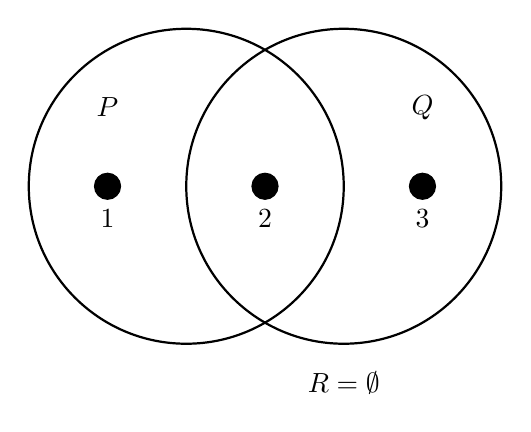
\begin{tikzpicture}
\def\circleA{(0,0) circle (2cm)}
\def\circleB{(0:2cm) circle (2cm)}
		%\begin{scope}
		%\clip \circleA;
		%\clip \circleB;
		%\fill[red!50] \circleA;
		%\end{scope}
		\draw[thick] \circleA;
    \node at (-1,1) {$P$};
    \node at (3,1) {$Q$};
    \node at (2,-2.5) {$R = \emptyset$};
		\draw[thick] \circleB;
    \node[circle,fill,draw,label={below:$1$}] at (-1,0) {};
    \node[circle,fill,draw,label={below:$2$}] at (1,0) {};
    \node[circle,fill,draw,label={below:$3$}] at (3,0) {};
\end{tikzpicture}
\end{frame}

\begin{frame}
\frametitle{(In)validity of arguments}

\begin{earg}
\item[] $\forall x(G(x) \eor E(x))$
\item[] $\enot \forall x\, V(x)$
\item[] $\forall x (E(x) \eif V(x))$
\item[\therefore] $\exists x (H(x) \eand G(x))$
\end{earg}

\begin{ekey}
\item[$Domain$] $1$, $2$
\item[G(x)] $1$
\item[E(x)] $2$
\item[V(x)] $2$
\item[H(x)] $2$
\end{ekey}

\vspace{-3cm}\hfill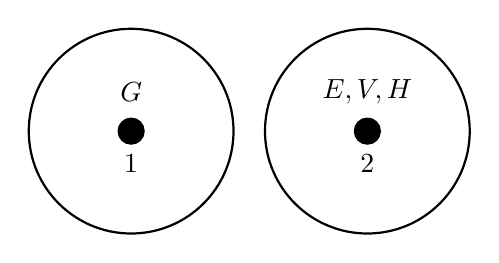
\begin{tikzpicture}
    \node at (-1.5,.5) {$G$};
    \node at (1.5,.5) {$E, V, H$};
		\draw[thick] (1.5,0) circle (1.3cm);
    \draw[thick] (-1.5,0) circle (1.3cm);
    \node[circle,fill,draw,label={below:$1$}] at (-1.5,0) {};
    \node[circle,fill,draw,label={below:$2$}] at (1.5,0) {};
\end{tikzpicture}

\end{frame}


\begin{frame}
\frametitle{Extensions of predicates}

\begin{ekey}
\item[$Domain$] $1$, $2$, $3$
\item[$a$] $1$
\item[A(x, y)] $\langle 1, 1\rangle$, $\langle 1,2\rangle$, $\langle 1,3\rangle$, $\langle 2,3\rangle$
\end{ekey}
\usetikzlibrary{arrows}
\hfill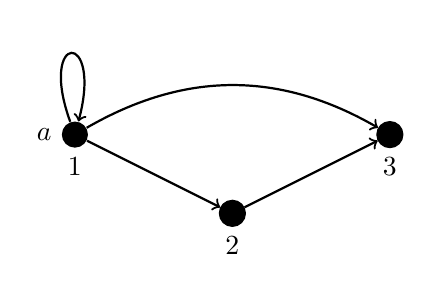
\begin{tikzpicture}
    \node[circle,fill,label={below:$1$},label={left:$a$}] (A) at (-1,0) {};
    \node[circle,fill,draw,label={below:$2$}] (B) at (1,-1) {};
    \node[circle,fill,draw,label={below:$3$}] (C) at (3,0) {};
    \draw[->,thick] (A) to[loop above,looseness=30,out=110] (A);
    \draw[->,thick] (A) -- (B);
    \draw[->,thick] (A) to[bend left] (C);
    \draw[->,thick] (B) -- (C);
\end{tikzpicture}
\end{frame}

\newhourlecture
\subsection{Truth of sentences of FOL}

\begin{frame}
  \frametitle{Truth of sentences of FOL}

  \begin{itemize}[<+->]
    \item Given an interpretation $I$ \dots
    \item An \emph{atomic sentence} is true iff the referents of the constants are in the extension of the predicate:
    \begin{itemize}
    \item $P(a)$ is true iff referent $r$ of $a$ is in extension of $P$
    \item $R(a,b)$ is true iff $\langle r,p\rangle$ is in extension of $R$\\
    (where $r$ is referent of $a$, $p$ is referent of $b$)
    \end{itemize}
    \item $\enot\metav{A}$ is true iff $\metav{A}$ is false
    \item $\metav{A} \eor \metav{B}$ is true iff at least one of $\metav{A}$, $\metav{B}$ is true
    \item $\metav{A} \eand \metav{B}$ is true iff both $\metav{A}$, $\metav{B}$ are true
    \item $\metav{A} \eif \metav{B}$ is true iff $\metav{A}$ is false or $\metav{B}$ is true
  \end{itemize}
\end{frame}

\begin{frame}
  \frametitle{Truth of quantified sentences}

  \begin{itemize}[<+->]
    \item $\exists x\,\metav{A}(x)$ is true iff $\metav{A}(x)$ is \emph{satisfied} by \emph{at least one} object in the domain
    \begin{itemize}
      \item $o$ satisfies $\metav{A}(x)$ iff $\metav{A}(c)$ is true in interpretation just like $I$, but with $o$ as referent of $c$
    \end{itemize}
    \item $\forall x\,\metav{A}(x)$ is true iff $\metav{A}(x)$ is \emph{satisfied} by \emph{every} object in the domain
  \end{itemize}
\end{frame}

\begin{frame}
  \frametitle{Truth of quantified sentences}

  \begin{itemize}[<+->]
    \item $\exists x\,(\metav{A}(x) \eand \metav{B}(x))$ is true iff some object satisfies $\metav{A}(x) \eand \metav{B}(x)$
    \begin{itemize}
      \item $o$ satisfies $\metav{A}(x) \eand \metav{B}(x)$ iff it satisfies both $\metav{A}(x)$ and $\metav{B}(x)$
    \end{itemize}
    \item $\forall x\,(\metav{A}(x) \eif \metav{B}(x))$ is true iff every object satisfies $\metav{A}(x) \eif \metav{B}(x)$
    \begin{itemize}
      \item $o$ satisfies $\metav{A}(x) \eif \metav{B}(x)$ iff
      either
      \begin{itemize}
        \item $o$ does not satisfy $\metav{A}(x)$ or
        \item $o$ does satisfy $\metav{B}(x)$
      \end{itemize}
    \end{itemize}
  \end{itemize}
\end{frame}


\begin{frame}
\frametitle{Making ``Some $A$s are $B$s'' true}

\begin{columns}
  \begin{column}{.5\textwidth}
    \begin{itemize}
      \item $\exists x\,(A(x) \eand B(x))$
      \item Extension of $A$ and $B$ must have something in common.
      \item[] (Filled area must contain at least one object)
      \item $A$ and $B$ can overlap, be equal, or be contained.
      \item Same situations make ``No $A$s are $B$s'' \emph{false}.
    \end{itemize}
  \end{column}
  \begin{column}{.5\textwidth}
\only<1>{\begin{tikzpicture}
\def\circleA{(0,0) circle (1.5cm)}
\def\circleB{(0:1.5cm) circle (1.5cm)}
		\begin{scope}
		\clip \circleA;
		\clip \circleB;
		\fill[highlightbg] \circleA;
		\end{scope}
		\draw[thick] \circleA;
    \node at (-1,.5) {$A$};
    \node at (2.5,.5) {$B$};
		\draw[thick] \circleB;
\end{tikzpicture}}
\only<3>{\begin{tikzpicture}
  \def\circleA{(0,0) circle (2cm)}
  \def\circleB{(0:.5cm) circle (1cm)}
      \begin{scope}
      \clip \circleA;
      \clip \circleB;
      \fill[highlightbg] \circleA;
      \end{scope}
      \draw[thick] \circleA;
      \node at (-1,1) {$A$};
      \node at (0,.5) {$B$};
      \draw[thick] \circleB;
  \end{tikzpicture}}
\only<2>{\begin{tikzpicture}
  \def\circleA{(0,0) circle (2cm)}
  \def\circleB{(0:.5cm) circle (1cm)}
      %\begin{scope}
      %\clip \circleA;
      %\clip \circleB;
      %\fill[highlightbg] \circleA;
      %\end{scope}
      \draw[thick,fill=highlightbg] \circleA;
      %\node at (-1,1) {};
      \node at (0,.5) {$A = B$};
      %\draw[thick] \circleB;
  \end{tikzpicture}}
  \only<4>{\begin{tikzpicture}
    \def\circleA{(0,0) circle (2cm)}
    \def\circleB{(0:.5cm) circle (1cm)}
        \begin{scope}
        \clip \circleA;
        \clip \circleB;
        \fill[highlightbg] \circleA;
        \end{scope}
        \draw[thick] \circleA;
        \node at (-1,1) {$B$};
        \node at (0,.5) {$A$};
        \draw[thick] \circleB;
    \end{tikzpicture}}
\end{column}
\end{columns}
\end{frame}

\begin{frame}
\frametitle{Making ``Some $A$s are $B$s'' false}

\begin{columns}
  \begin{column}{.5\textwidth}
    \begin{itemize}
      \item $\enot\exists x\,(A(x) \eand B(x))$
      \item Extension of $A$ and $B$ must have nothing in common.
      \item $A$ and $B$ don't overlap, or one or both is empty.
      \item Same situations make ``No $A$s are $B$s'' \emph{true}.
    \end{itemize}
  \end{column}
  \begin{column}{.5\textwidth}
\only<1>{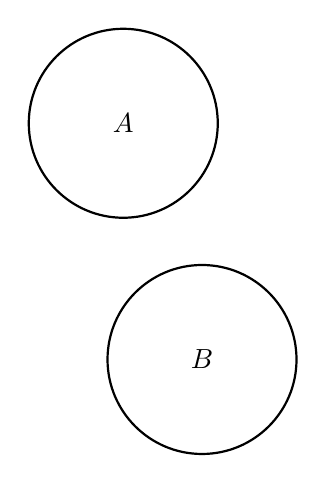
\begin{tikzpicture}
\def\circleA{(1,0) circle (1.2cm)}
\def\circleB{(0,3) circle (1.2cm)}
		\draw[thick] \circleA;
    \node at (1,0) {$B$};
    \node at (0,3) {$A$};
		\draw[thick] \circleB;
\end{tikzpicture}}
\only<2>{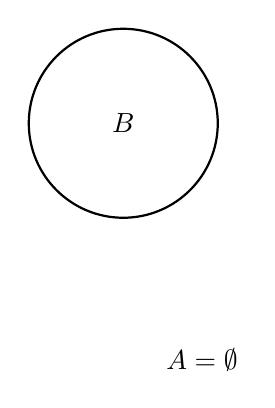
\begin{tikzpicture}
  \def\circleA{(1,0) circle (1.2cm)}
  \def\circleB{(0,3) circle (1.2cm)}
      %\draw[thick] \circleA;
      \node at (1,0) {$A=\emptyset$};
      \node at (0,3) {$B$};
      \draw[thick] \circleB;
  \end{tikzpicture}}
\only<3>{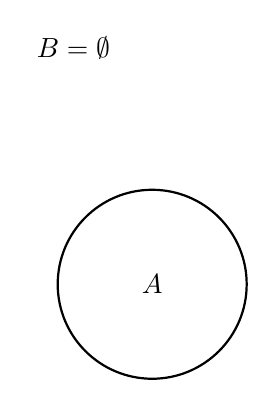
\begin{tikzpicture}
\def\circleA{(1,0) circle (1.2cm)}
\def\circleB{(0,3) circle (1.2cm)}
		\draw[thick] \circleA;
    \node at (1,0) {$A$};
    \node at (0,3) {$B=\emptyset$};
		%\draw[thick] \circleB;
\end{tikzpicture}}
\only<4>{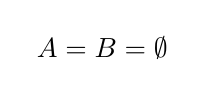
\begin{tikzpicture}
  %\def\circleA{(1,0) circle (1.2cm)}
  %\def\circleB{(0,3) circle (1.2cm)}
  %    \draw[thick] \circleA;
  %    \node at (1,0) {$A$};
      \node at (0,3) {$A= B=\emptyset$};
      %\draw[thick] \circleB;
  \end{tikzpicture}}
\end{column}
\end{columns}
\end{frame}

\begin{frame}
\frametitle{Making ``All $A$s are $B$s'' true}

\begin{columns}
  \begin{column}{.5\textwidth}
    \begin{itemize}
      \item $\forall x\,(A(x) \eif B(x))$
      \item Extension of $A$ must be contained in extension of $B$.
      \item Extensions of $A$ and $B$ can be the same.
      \item Extension of $A$ can be empty.
      \item Same situations make \dots
      \begin{itemize}
        \item ``Only $B$s are $A$s'' \emph{true}.
        \item ``Some $A$s are not $B$s'' \emph{false}.
      \end{itemize}
    \end{itemize}
  \end{column}
  \begin{column}{.5\textwidth}
\only<1>{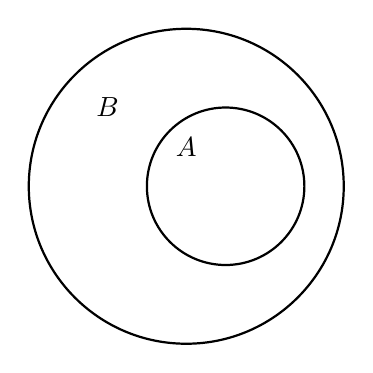
\begin{tikzpicture}
  \def\circleA{(0,0) circle (2cm)}
  \def\circleB{(0:.5cm) circle (1cm)}
      %\begin{scope}
      %\clip \circleA;
      %\clip \circleB;
      %\fill \circleA;
      %\end{scope}
      \draw[thick] \circleA;
      \node at (-1,1) {$B$};
      \node at (0,.5) {$A$};
      \draw[thick] \circleB;
  \end{tikzpicture}}
\only<2>{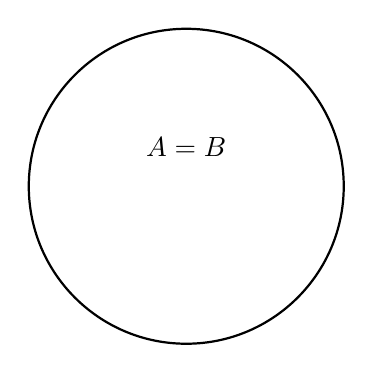
\begin{tikzpicture}
  \def\circleA{(0,0) circle (2cm)}
  \def\circleB{(0:.5cm) circle (1cm)}
      %\begin{scope}
      %\clip \circleA;
      %\clip \circleB;
      %\fill[highlightbg] \circleA;
      %\end{scope}
      \draw[thick] \circleA;
%      \node at (-1,1) {$B=A$};
      \node at (0,.5) {$A=B$};
      %\draw[thick] \circleB;
  \end{tikzpicture}}
\only<3>{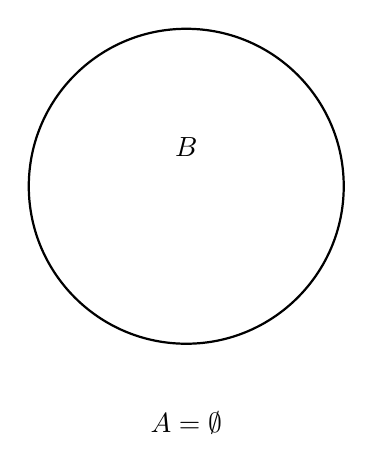
\begin{tikzpicture}
  \def\circleA{(0,0) circle (2cm)}
  \def\circleB{(0:.5cm) circle (1cm)}
      %\begin{scope}
      %\clip \circleA;
      %\clip \circleB;
      %\fill[highlightbg] \circleA;
      %\end{scope}
      \draw[thick] \circleA;
      \node at (0,.5) {$B$};
      \node at (0,-3) {$A=\emptyset$};
      %\draw[thick] \circleB;
  \end{tikzpicture}}
\end{column}
\end{columns}
\end{frame}

\begin{frame}
\frametitle{Making ``All $A$s are $B$s'' false}

\begin{columns}
  \begin{column}{.5\textwidth}
    \begin{itemize}
      \item $\forall x\,(A(x) \eif B(x))$
      \item Extension of $A$ must contain something not in $B$.
      \item Extensions of $A$ cannot be empty, but $B$ may be empty.
      \item Same situations make \dots
    \begin{itemize}
        \item ``Only $B$s are $A$s'' \emph{false}.
        \item ``Some $A$s are not $B$s'' \emph{true}.
      \end{itemize}
    \end{itemize}
  \end{column}
  \begin{column}{.5\textwidth}
\only<1>{\begin{tikzpicture}
\def\circleA{(0,0) circle (1.5cm)}
\def\circleB{(0:1.5cm) circle (1.5cm)}
		\begin{scope}[even odd rule]
		\clip \circleB (0,0) circle (2cm);
		\fill[highlightbg] \circleA;
		\end{scope}
		\draw[thick] \circleA;
    \node at (-1,.5) {$A$};
    \node at (2.5,.5) {$B$};
		\draw[thick] \circleB;
\end{tikzpicture}}
\only<2>{\begin{tikzpicture}
\def\circleA{(1,0) circle (1.2cm)}
\def\circleB{(0,3) circle (1.2cm)}
		\draw[thick] \circleA;
		\draw[thick,fill=highlightbg] \circleB;\node at (1,0) {$B$};\node at (0,3) {$A$};
\end{tikzpicture}}
\only<3>{\begin{tikzpicture}
\def\circleA{(0,0) circle (1.5cm)}
\def\circleB{(0:1.5cm) circle (1.5cm)}
		\begin{scope}
		\fill[highlightbg] \circleA;
		\end{scope}
		\draw[thick] \circleA;
    \node at (-1,.5) {$A$};
    \node at (2.5,.5) {$B=\emptyset$};
\end{tikzpicture}}
\end{column}
\end{columns}
\end{frame}


\subsection{Testing for validity}

\begin{frame}
\frametitle{Arguments involving quantifiers}

\begin{enumerate}[<+->]
\item If an action x is morally wrong then
A is blameworthy for freely doing x.
\item If x is rationally optimal (there is no action which A has
  reason to think there is more reason for A to do), then A is not
  blameworthy for freely doing x.
\item Therefore, if x is morally wrong, then
x is not rationally optimal.
(Principle of moral categoricity.)
\end{enumerate}

\begin{raggedleft}
\small(John Skorupski, \textit{Ethical Explorations}, 2000 (\href{http://books.google.ca/books?id=bxIzZYqRZdwC&lpg=PP1&pg=PA170\#v=onepage&q&f=false}{link})
 \end{raggedleft}

\end{frame}

\begin{frame}
  \frametitle{Symbolizing Skorupski}

  \begin{enumerate}
    \only<1-2>{\item[1.] If an action x is morally wrong then
    A is blameworthy for freely doing x.}
    \only<3-4>{\item[2.] If x is rationally optimal, then A is not
      blameworthy for freely doing x.}
    \only<5-6>{\item[3.] Therefore, if x is morally wrong, then
    x is not rationally optimal. }
    \end{enumerate}

  \begin{ekey}
  \item[$Domain$] actions
  \item[W(x)] $x$ is morally wrong
  \item[B(x)] A is blameworthy for freely doing $x$
  \item<3->[O(x)] $x$ is rationally optimal
  \end{ekey}
  \begin{earg}
  \item<1->[] \uncover<2->{\alert<2>{$\forall x(W(x) \eif B(x))$}}
  \item<3->[] \uncover<4->{\alert<4>{$\forall x(O(x) \to \lnot B(x))$}}
  \item<5->[\therefore] \uncover<6>{\alert<6>{$\forall x(W(x) \to \lnot O(x))$}}
  \end{earg}

  \end{frame}

\begin{frame}
\frametitle{Symbolizing Skorupski}

\begin{ekey}
\item[$Domain$] actions
\item[W(x)] $x$ is morally wrong
\item[B(x)] A is blameworthy for freely doing $x$
\item[O(x)] $x$ is rationally optimal
\end{ekey}
\begin{earg}
\item[] $\forall x(W(x) \eif B(x))$
\item[] $\forall x(O(x) \to \lnot B(x))$
\item[\therefore] $\forall x(W(x) \to \lnot O(x))$
\end{earg}

\begin{earg}
\item[] All Ws are Bs
\item[] No Os are Bs (iff No Bs are Os)
\item[\therefore] No Ws are Os
\end{earg}

\end{frame}

\begin{frame}{Determining validity}

  \begin{columns}
    \begin{column}{.5\textwidth}
      \begin{itemize}[<+->]
        \item Make conclusion $\forall x(W(x) \to \lnot O(x))$ false.
        \item Make $\exists x(W(x) \land O(x))$ true.
        \item Make $\forall x(W(x) \eif B(x))$ true.
        \item $\exists x(O(x) \land B(x))$ is now forced to be true.
        \item So, $\forall x(O(x) \to \lnot B(x))$ is false.
        \item But those are not the only possibilities!
      \end{itemize}
    \end{column}
    \begin{column}{.5\textwidth}
\only<2->{\begin{tikzpicture}
  \def\circleA{(0,0) circle (1.5cm)}
  \def\circleB{(0:1.5cm) circle (1.5cm)}
  \def\circleC{(0,0) circle (2.3cm)}
      \begin{scope}
      \clip \circleA;
      \clip \circleB;
      \fill[highlightbg] \circleA;
      \end{scope}
      \draw[thick] \circleA;
      \node at (-1,.5) {$W$};
      \node at (2.5,.5) {$O$};
      \draw[thick] \circleB;
      \uncover<3->{\draw[thick] \circleC;
      \node at (-1.7,.5) {$B$};}
\end{tikzpicture}}
\end{column}
\end{columns}
\end{frame}

\begin{frame}{Other configurations}
  \begin{columns}
  \begin{column}{.4\textwidth}
  \begin{tikzpicture}
    \def\circleA{(0,0) circle (1.5cm)}
    \def\circleB{(0:1.5cm) circle (1.5cm)}
    \def\circleC{(.6,0) circle (2.8cm)}
        \begin{scope}
        \clip \circleA;
        \clip \circleB;
        \fill[highlightbg] \circleA;
        \end{scope}
        \draw[thick] \circleA;
        \node at (-1,.5) {$W$};
        \node at (2.5,.5) {$O$};
        \draw[thick] \circleB;
        \draw[thick] \circleC;
        \node at (-1.7,.5) {$B$};
  \end{tikzpicture}
\end{column}
\begin{column}{.6\textwidth}
  \vspace*{2ex}
  
  \begin{tikzpicture}
    \def\circleA{(0,0) circle (1.5cm)}
    \def\circleB{(0:1.5cm) circle (1.5cm)}
        \begin{scope}
        \clip \circleA;
        \clip \circleB;
        \fill[highlightbg] \circleA;
        \end{scope}
        \draw[thick] \circleA;
        \node at (-.8,0) {$W = B$};
        \node at (2.5,0) {$O$};
        \draw[thick] \circleB;
  \end{tikzpicture}
\\[-2ex]
\hfill\begin{tikzpicture}
    \def\circleA{(0,0) circle (1cm)}
    \def\circleC{(0,0) circle (2cm)}
        \fill[highlightbg] \circleA;
        \draw[thick] \circleA;
        \node at (0,0) {$W = O$};
        \draw[thick] \circleC;
        \node at (-1.5,0) {$B$};
  \end{tikzpicture}
\end{column}
\end{columns}
\end{frame}

\newhourlecture

\subsection{Semantic notions in FOL}

\begin{frame}
\frametitle{Semantics notions in FOL}

\begin{itemize}[<+->]
  \item $\metav{P}_1,\dots,\metav{P}_n \mathrel{\emph{$\boldsymbol\models$}} \metav{Q}$ if no interpretation
  makes all of $\metav{P}_1,\dots,\metav{P}_n$ true and $\metav{Q}$~false.
  \item $\metav{P}$ is a \emph{validity} ($\models \metav{P}$) if it is true in every interpretation.
  \item $\metav{P}$ and $\metav{Q}$ are \emph{equivalent in FOL} if no
 interpretation makes one true but the other false.
 \item $\metav{P}_1,\dots,\metav{P}_n$ are \emph{jointly satisfiable
 in FOL} if some interpretation makes all of them true at the same time.
\end{itemize}
\end{frame}

\begin{frame}
\frametitle{Using interpretations}

\begin{itemize}[<+->]
\item By providing one suitable interpretation we \emph{can} show that\dots
\begin{itemize}[<+->]
  \item an argument is \emph{not valid} in FOL
  \item a sentence is \emph{not a validity} in FOL
  \item two sentences are \emph{not equivalent} in FOL
  \item some sentences \emph{are satisfiable} in FOL
\end{itemize}
\item But we \emph{cannot} show using any number of interpretations that\dots
\begin{itemize}[<+->]
  \item an argument \emph{is valid} in FOL
  \item a sentence \emph{is a validity} in FOL
  \item two sentences \emph{are equivalent} in FOL
  \item some sentences \emph{are not satisfiable} in FOL
\end{itemize}
\end{itemize}
\end{frame}

\begin{frame}
\frametitle{Examples}

\begin{itemize}[<+->]
  \item $\forall x(A(x) \eor B(x))$ and $\forall x\,A(x) \eor \forall x\,B(x)$ are not equivalent.
  \item  $\forall x(A(x) \eif B(x)), \forall x(A(x) \eif \enot B(x))$ are jointly satisfiable.
  \item $\forall x(\enot A(x) \eif B(x)), \exists x(B(x) \eand C(x,b))
  \not\models \exists x(\enot A(x) \eand C(x,b))$.
  \item $\not\models \exists x\, A(a,x) \eif \exists x\, A(x,x)$.
\end{itemize}
Test solutions on \href{https://carnap.io/shared/rzach@ucalgary.ca/Practice\%20Problems\%20VI.md}{carnap.io}
\end{frame}

\subsection{Arguing about interpretations}

\begin{frame}
\frametitle{Arguing about Interpretations}

\begin{itemize}[<+->]
  \item No interpretation(s) can show that an argument is valid.
  \item That's because there is no way to inspect all possible interpretations.
  \item But we can show that arguments are valid, by:
  \begin{itemize}
    \item a formal proof (next time)
    \item an informal argument
  \end{itemize}
  \item The informal argument makes use of the \emph{truth conditions}
  for sentences of FOL.
  \item Analogous to arguing about valuations in TFL.
\end{itemize}

\end{frame}

\begin{frame}
  \frametitle{Example}

  \[\forall x\,\metav{A}(x) \lor \forall x\,\metav{B}(x) \models \forall x(\metav{A}(x) \lor \metav{B}(x))\]
  \begin{itemize}[<+->]
  \item Suppose an interpretation makes premise $\forall x\,\metav{A}(x)
  \lor \forall x\,\metav{B}(x)$ true.
  \item By the truth conditions for $\lor$, it makes either $\forall x\,\metav{A}(x)$ or $\forall
  x\,\metav{B}(x)$ true.
  \item Suppose it's the first, i.e., $\forall x\,\metav{A}(x)$ is true.
    \begin{itemize}[<+->]
      \item By the truth conditions for $\forall$, every object in the domain satisfies $\metav{A}(x)$.
      \item By the truth conditions for $\lor$, every object satisfies $\metav{A}(x) \lor \metav{B}(x)$
      \item So, by the truth conditions for $\forall$, $\forall x(\metav{A}(x)
      \lor \metav{B}(x))$ is true.
    \end{itemize}
  \item Suppose it's the second, i.e., $\forall
  x\,\metav{B}(x)$ is true: Similarly.
  \item These are the only possibilities: the interpretation must make the conclusion also true.
  \end{itemize}
\end{frame}

\newhourlecture
\newonlinelecture

\section{Proofs in FOL}

\subsection{Rules for $\forall$}

\begin{frame}
\frametitle{Rules for formal proofs}

\begin{itemize}[<+->]
\item Need rules for $\forall$ and $\exists$ for formal proofs
\item Formal proofs now more important, because no alternative
  (truth-table method)
\item Intro and Elim rules should be
\begin{itemize}[<+->]
\item simple
\item elegant (not involve other connectives or quantifiers)
\item yield only valid arguments
\end{itemize}
\end{itemize}

\end{frame}

\begin{frame}
\frametitle{Candidates for rules}

\begin{itemize}[<+->]
\item Only simple sentence close to $\forall x\, \metav A(\metav x)$ is
$\metav A(\metav c)$
\item Gives simple, elegant $\forall$E rule:

\begin{fitchproof}
\have[k]{a}{\forall \metav x\, \metav A(\metav x)}
\have[ ]{b}{\metav A(\metav c)}\Ae{a}
\end{fitchproof}
\item This is a good rule: $\forall \metav x\,\metav A(\metav x)
\models \metav A(\metav c)$.
\end{itemize}
\end{frame}

\begin{frame}
  \frametitle{Candidates for rules}

\begin{itemize}[<+->]
\item Problem: corresponding ``intro rule'' isn't valid:
\begin{fitchproof}
\have[k]{a}{\metav A(\metav c)}
\have[ ]{b}{\forall \metav x\,\metav A(\metav x)}\by{\emph{doesn't follow from}}{a}
\end{fitchproof}
\item Diagnosis: the $\metav c$ in $\metav A(\metav c)$ is a name for
a \emph{specific object}.
\item We need a name for an \emph{arbitrary,
unspecified object}.
\item If $\metav A(\metav c)$ is true for whatever $\metav c$
\emph{could} name, then $\metav A(\metav x)$ is satisfied by \emph{every} object.
\end{itemize}
\end{frame}

\begin{frame}
\frametitle{Names for arbitrary objects}

\begin{itemize}[<+->]
\item When we give proofs of general claims, we often do use names for
arbitrary objects (well, mathematicians do at least).

\begin{earg}
\item[] All heroes admire Greta.
\item[] Only people who wear capes admire Greta.
\item[\therefore] All heroes wear capes.
\end{earg}
\pause
Proof: Let Carl be any hero.  Since all heroes admire Greta, Carl
admires Greta. Since only people who wear capes admire Greta, Carl is
wears a cape. But ``Carl'' stands for \emph{any} hero. So all heroes
wear capes.
\end{itemize}
\end{frame}

\begin{frame}
  \frametitle{Universal generalization}

\begin{fitchproof}
  \have[k]{a}{\metav{A}(\metav{c})}
  \have[ ]{b}{\forall \metav{x}\,\metav{A}(\metav{x})}\Ai{a}
\end{fitchproof}
  \begin{itemize}[<+->]
  \item $\metav{c}$ is special: $\metav{c}$ must not appear in any
  premise or assumption of a subproof not already ended
  \item $\metav{A}(\metav{x})$ is obtained from $\metav{A}(\metav{c})$ by replacing \emph{all} occurrences of $\metav{c}$ by $\metav{x}$.
  \item In other words, $\metav{c}$ must also not occur in $\forall
  \metav{x}\,\metav{A}(\metav{x})$.
 \end{itemize}
\end{frame}

\begin{frame}
\frametitle{General conditional proof}

Proving ``All $A$s are $B$s''

\begin{fitchproof}
  \open
  \hypo[k]{a}{A(c)}
  \have[l]{b}{B(c)}
  \close
  \have{c}{A(c) \eif B(c)}\ci{a-b}
  \have{d}{\forall x(A(x) \eif B(x))}\Ai{c}
\end{fitchproof}
\end{frame}

\begin{frame}
\frametitle{Example}

\begin{earg}
  \item[] All heroes admire Greta.
  \item[] Only people who wear capes admire Greta.
  \item[\therefore] All heroes wear capes.
\end{earg}

\bigskip

\begin{earg}
  \item[] $\forall x(H(x) \eif A(x,g))$
  \item[] $\forall x(A(x,g) \eif C(x))$
  \item[\therefore] $\forall x(H(x) \eif C(x))$
\end{earg}

Let's do it on \href{https://carnap.io/shared/rzach@ucalgary.ca/Practice\%20Problems\%20VII.md}{carnap.io}
\end{frame}

\begin{frame}
\frametitle{Example}
\small
\begin{fitchproof}
  \hypo{a}{\forall x(H(x) \eif A(x,g))}
  \hypo{b}{\forall x(A(x,g) \eif C(x))}
  \open
  \hypo{c}{H(c)}
  \have{d}{H(c) \eif A(c,g)}\Ae{a}
  \have{e}{A(c,g)}\ce{d,c}
  \have{f}{A(c,g) \eif C(c)}\Ae{b}
  \have{g}{C(c)}\ce{f,e}
  \close
  \have{h}{H(c) \eif C(c)}\ci{c-g}
  \have{i}{\forall x(H(x) \eif C(x))}\Ai{h}
\end{fitchproof}
\end{frame}

\begin{frame}
  \frametitle{Example}
  \small
  \begin{fitchproof}
    \hypo{1}{\forall x\,A(x) \eor \forall x\, B(x)}
    \open
    \hypo{2}{\forall x\,A(x)}
    \have{3}{A(c)}\Ae{2}
    \have{4}{A(c) \eor B(c)}\oi{3}
\close
\open
\hypo{5}{\forall x\,B(x)}
\have{6}{B(c)}\Ae{5}
\have{7}{A(c) \eor B(c)}\oi{6}
\close
  \have{8}{A(c) \eor B(c)}\oe{1,2-4,5-7}
  \have{9}{\forall x(A(x) \eor B(x))}\Ai{8}
  \end{fitchproof}
  \end{frame}

\newhourlecture
\subsection{Rules for $\exists$}

\begin{frame}
\frametitle{Rules for $\exists$}

\begin{itemize}[<+->]
\item If we know of a specific object that it satisfies $\metav A(x)$, we know that at least one object satisfies $\metav A(x)$.
\item So this rule is valid:
\begin{fitchproof}
  \have[k]{a}{\metav A(\metav c)}
  \have[ ]{b}{\exists \metav x\, \metav A(\metav x)}\Ei{a}
\end{fitchproof}
\end{itemize}
\end{frame}

\begin{frame}
\frametitle{Arbitrary objects again}

\begin{itemize}
  \item Problem: corresponding ``elim rule'' isn't valid:
  \begin{fitchproof}
    \have[k]{a}{\exists \metav x\, \metav A(\metav x)}
    \have[ ]{b}{\metav A(\metav c)}\by{\emph{doesn't follow from}}{a}
  \end{fitchproof}
  \item If we know that $\exists \metav x\, \metav A(\metav x)$ is
  true, we know that \emph{some} objects satisfy $\metav A(\metav x)$,
  but not which ones.
\item To use this information, we have to introduce a temporary name
that stands for any one of the objects that satisfy $\metav A(\metav
x)$.
\end{itemize}
\end{frame}

\begin{frame}
  \frametitle{Reasoning from existential information}

  \begin{itemize}
    \item To use $\exists \metav x\,\metav A(\metav x)$, pretend the
    $\metav x$ has a name~$\metav c$, and reason from $\metav A(\metav
    c)$.
    \item This is what we'd do if we reason informally from existential information, e.g.,
  \begin{earg}
  \item[] There are heroes who wear capes.
  \item[] Anyone who wears a cape admires Greta.
  \item[\therefore] Some heroes admire Greta.
  \end{earg}

\pause
Proof: We know there are heroes who wear capes. Let Cate be an
arbitrary one of them.  So Cate wears a cape. Since anyone who wears a
cape admires Greta, Cate admires Greta. Since Cate is a hero who
admires Greta, some heroes admire Greta.
\end{itemize}

\end{frame}

\begin{frame}
\frametitle{Existential elimination}

\begin{itemize}[<+->]
  \item If
  \begin{itemize}[<+->]
    \item we know that some object satisfies $\metav A(\metav x)$,
    \item we assume for the time being that $c$ is one of them (i.e.,
  assume $\metav A(\metav c)$), and
    \item we can prove that $\metav B$ follows from this assumption,
\end{itemize}
\item[] then $\metav B$ follows already from $\exists \metav x\, \metav A(\metav x)$.
\item Rule for existential elimination:

\begin{fitchproof}
  \have[k]{a}{\exists \metav x\, \metav A(\metav x)}
  \open
  \hypo[m]{b}{\metav A(\metav c)}
  \have[n]{c}{\metav B}
\close
\have[ ]{d}{\metav B}\Ee{a,b-c}
\end{fitchproof}
\item $\metav c$ is special: $\metav c$ must not appear outside subproof
\end{itemize}
\end{frame}

\begin{frame}
\frametitle{Example}

\begin{earg}
  \item[] There are heroes who wear capes.
  \item[] Anyone who wears a cape admires Greta.
  \item[\therefore] Some heroes admire Greta.
\end{earg}
\bigskip
\begin{earg}
  \item[] $\exists x(H(x) \eand C(x))$
  \item[] $\forall x(C(x) \eif A(x,g)$
  \item[\therefore] $\exists x(H(x) \eand A(x,g))$
\end{earg}
\end{frame}

\begin{frame}
\frametitle{Example}
\small
\begin{fitchproof}
  \hypo{a}{\exists x(H(x) \eand C(x))}
  \hypo{b}{\forall x(C(x) \eif A(x,g)}
  \open
  \hypo{c}{H(c) \eand C(c)}
  \have{d}{C(c)}\ae{c}
  \have{e}{C(c) \eif A(c,g)}\Ae{b}
  \have{f}{A(c,g)}\ce{d,e}
  \have{g}{H(c)}\ae{c}
  \have{h}{H(c) \eand A(c,g)}\ai{d,g}
  \have{i}{\exists x(H(x) \eand A(x,g))}\Ei{h}
  \close
  \have{j}{\exists x(H(x) \eand A(x,g))}\Ei{a,c-i}
\end{fitchproof}
\end{frame}


\newhourlecture
\newonlinelecture

\section{Multiple quantifiers}

\subsection{Two quantifiers}

\begin{frame}
  \frametitle{Formulas expressing relations}

\begin{itemize}[<+->]
  \item A formula $\metav{A}(x)$ with one free variable expresses a \emph{property}.
  \item A formula $\metav{B}(x, y)$ with two free variables expresses a \emph{relation}
  \item $\forall x\forall y\, \metav{B}(x, y)$ is a sentence; 
  \item It's true iff 
  \emph{every pair} of objects $\alpha$, $\beta$ stand in the relation expressed by $\metav{B}(x, y)$.
  \item $\exists x\exists y\, \metav{B}(x, y)$ is a sentence.
  \item It's true iff
  \emph{at least one pair} of objects $\alpha$, $\beta$ stand in the relation expressed by $\metav{B}(x, y)$.
\end{itemize}
\end{frame}

\begin{frame}
  \frametitle{Multiple uses of a single quantifier: $\forall$}

\begin{itemize}[<+->]
  \item $A(x, y)$ \dots $x$ admires $y$.
  \item $\forall x\forall y\, A(x, y)$ \dots for every pair $\langle
  \alpha,\beta\rangle$, $\alpha$ admires $\beta$.
  \item In other words: everyone admires everyone.
  \item Note: ``every pair'' includes pairs $\langle\alpha, \alpha\rangle$, i.e.,
  \item $\forall x\forall y\, A(x, y)$ is true only if all pairs $\langle \alert{\alpha, \alpha}\rangle$ satisfy $A(x, y)$.
  \item That means, everyone admires themselves, in addition to everyone else.
  \item So: $\forall x\forall y\, A(x, y)$ does \emph{not} symbolize ``everyone admires everyone \emph{else}.''
\end{itemize}

\end{frame}

\begin{frame}
  \frametitle{Multiple uses of single quantifier: $\exists$}

\begin{itemize}[<+->]
  \item $\exists x\exists y\, A(x, y)$ \dots for at least one pair $\langle \alpha,\beta\rangle$, $\alpha$ admires $\beta$.
  \item In other words: at least one person admires at least one person.
  \item Note: includes pairs $\langle\alpha, \alpha\rangle$, i.e.,
  \item $\exists x\exists y\, A(x, y)$ is already true if a single pair $\langle \alpha, \alpha\rangle$ satisfies $ A(x, y)$.
  \item That means, we could just have one person admiring themselves.
  \item So: $\exists x\exists y\, A(x, y)$ does \emph{not} symbolize ``someone admires someone \emph{else}.''
\end{itemize}
\end{frame}

\begin{frame}
    \frametitle{Alternating quantifiers}

\begin{enumerate}[<+->]
  \item $\forall x \exists y \, A(x, y)$
  \item<2->[] Everyone admires someone\\
    (possibly themselves)
  \item $\forall y \exists x \, A(x, y)$
  \item<3->[] Everyone is admired by someone\\
  (not necessarily the same person)
  \item $\exists x \forall y \, A(x, y)$
  \item<4->[] Someone admires everyone\\
  (including themselves)
  \item $\exists y \forall x \, A(x, y)$
  \item<5->[] Someone is admired by everyone\\
    (including themselves)
\end{enumerate}

\end{frame}

\begin{frame}
    \frametitle{Convergence vs. uniform convergence}

\begin{itemize}[<+->]
\item A function $f$ \emph{point-wise continuous} if
\[
\forall \epsilon\forall x\forall y\exists \delta(\left|x - y\right| < \delta \to \left|f(x) - f(y)\right| < \epsilon)
\]
\item A function $f$ \emph{uniformly continuous} if
\[
\forall \epsilon\exists \delta\forall x\forall y(\left|x - y\right| < \delta \to \left|f(x) - f(y)\right| < \epsilon)
\]
\end{itemize}

\end{frame}

\subsection{Using quantifiers to express properties}

\begin{frame}
\frametitle{Our symbolization key}

    \begin{ekey}
    \item[$Domain$] people alive in \lecyear{} and items of clothing
    \item[a] Autumn
    \item[g] Greta
    \item[P(x)] \gap{x} is a person
    \item[L(x)] \gap{x} is an item of clothing.
    \item[E(x)] \gap{x} is a cape
    \item[R(x,y)] \gap{x} wears \gap{y}
    \item[H(x)] \gap{x} is a hero
    \item[I(x)] \gap{x} inspires
    \item[Y(x, y)] \gap{x} is younger than \gap{y}
    \item[A(x, y)] \gap{x} admires \gap{y}
    \item[O(x, y)] \gap{x} owns \gap{y}
    \end{ekey}
\end{frame}


\begin{frame}
  \frametitle{Expressing properties, revisited}
    \begin{itemize}[<+->]
      \item One-place predicates express properties, e.g.,
      \item[] $H(x)$ expresses property ``being a hero''
      \item Combinations of predicates (with connectives, names) can
      express derived properties, e.g.,
      \begin{itemize}[<+->]
        \item[] $A(x, g)$ expresses ``$x$ admires Greta''
        \item[] $H(x) \eand C(x)$ expresses ``$x$ is a hero who wears a cape''
      \end{itemize}
    \item Using quantifiers, we can express even more complex
    properties, e.g.,
    \item[] $\exists y(P(y) \eand A(x, y))$ expresses ``$x$ admires someone''
    \end{itemize}
  \end{frame}
  
  \begin{frame}
    \frametitle{Finding, using properties expressed}
  
  \begin{itemize}[<+->]
    \item If you can say it for Greta, you can say it for $x$.
    \begin{itemize}[<+->]
      \item Greta admires a hero.
      \item[] \alert{$\exists y(H(y) \eand A(g, y))$}
      \item $x$ admires a hero.
      \item[] \alert{$\exists y(H(y) \eand A(x, y))$}
    \end{itemize}
    \item If you can say it for $x$, you can say it for Greta.
    \begin{itemize}[<+->]
      \item $x$ wears a cape.
      \item[] \alert{$\exists y(E(y) \eand R(x,y))$}
      \item Greta wears a cape.
      \item[] \alert{$\exists y(E(y) \eand R(g,y))$}
    \end{itemize}
  \end{itemize}
  \begin{ekey}\scriptsize
    \item[E(x)] \gap{x} is a cape
    \item[R(x,y)] \gap{x} wears \gap{y}
  \end{ekey}
  \end{frame}
  
  \begin{frame}
  \frametitle{Examples}
  
  \begin{itemize}[<+->]
    \item $x$ wears a cape.
    \item[] \alert{$\exists y(E(y) \eand R(x,y))$}
    \item $x$ is admired by everyone.
    \item[] \alert{$\forall y(P(y) \eif A(y,x))$}
    \item $x$ admires a hero.
    \item[] \alert{$\exists y(H(y) \eand A(x, y))$}
    \item $x$ admires only heroes.
    \item[] \alert{$\forall y(A(x, y) \eif H(y))$}
    \item $x$ is naked.
    \item[] \alert{$\enot\exists y(L(y) \eand R(x,y))$}\\
     \alert{$\forall y(L(y) \eif \enot R(x,y))$}
  \end{itemize}
  
  {\scriptsize
  \begin{tabular}{llll}
    $P(x)$ & \gap{x} is a person &
    $L(x)$ & \gap{x} is an item of clothing\\
    $E(x)$ & \gap{x} is a cape &
    $R(x,y)$ & \gap{x} wears \gap{y}
  \end{tabular}}
  \end{frame}

\subsection{Multiple determiners}

\begin{frame}
  \frametitle{Symbolizing multiple determiners}

\begin{itemize}[<+->]
\item What if your sentence contains more than one determiner phrase?
\item Deal with each determiner separately!
\item Think of determiner phrase as replaced with name or variable---result has one less determiner.
\item When you're down to one determiner, apply known methods for single quantifiers.
\item This results in formulas that express properties or relations, but themselves contain quantifiers.
\end{itemize}
\end{frame}

\begin{frame}
    \frametitle{Two separate determiner phrases}

\begin{itemize}[<+->]
\item \textcolor{highlightB}{All heroes} wear \textcolor{highlightA}{a cape}
\item \textcolor{highlightB}{All heroes} satisfy ``$x$ wears \textcolor{highlightA}{a cape}'' \[
\textcolor{highlightB}{\forall x(H(x) \eif {}} \text{``$x$ wears \textcolor{highlightA}{a cape}''})
\]
\item $x$ wears \textcolor{highlightA}{a cape}\[
 \textcolor{highlightA}{\exists y(E(y) \land{}} R(x, y))
\]
\item Together:
\[
\textcolor{highlightB}{\forall x(H(x) \eif {}} \textcolor{highlightA}{\exists y(E(y) \land{}} R(x, y)))
\]
\end{itemize}
\end{frame}

\begin{frame}
    \frametitle{Determiner within determiner phrase}

\begin{itemize}[<+->]
\item \textcolor{highlightB}{All heroes who wear \textcolor{highlightA}{ a cape}} admire Greta.
\item All things that satisfy ``$x$ is a hero who wears \textcolor{highlightA}{a cape}'' admire Greta.
\[
\forall x (\text{``x is a hero who wears a cape''} \eif A(x,g))
\]
\item $x$ is a hero who wears \textcolor{highlightA}{a cape}
\[
 H(x) \land \exists y(E(y) \land R(x, y))
\]
\item Together:
\[
\forall x((H(x) \land \exists y(E(y) \land R(x, y))) \eif A(x,g))
\]
\end{itemize}
\end{frame}

\begin{frame}
    \frametitle{Mary Astell, 1666--1731}

\begin{columns}
\begin{column}{3cm}
\pgfimage[height=4cm]{../assets/astell}
\end{column}
\begin{column}{7cm}
\begin{itemize}
\item British political philosopher
\item \textit{Some Reflections upon Marriage} (1700)
\item In preface to 3rd ed. 1706 reacts to William Nicholls' claim (in \textit{The Duty of Inferiors
towards their Superiors, in Five Practical Discourses} (London 1701), Discourse IV: The Duty of Wives to their
Husbands), that women are naturally inferior to men.
\end{itemize}
\end{column}
\end{columns}
\end{frame}



\begin{frame}
    \frametitle{Astell TL;DR}

\begin{itemize}
  \item What can Nicholls possibly mean by ``women are naturally inferior to men''?
  \item It can't be that some women is inferior to some man, since
  that's ``no great discovery.''
  \item After all, surely some men are inferior to some women.
  \item The obviously intended meaning must be: \emph{all} women are
  inferior to \emph{all} men.
  \item But that can't be right, for then ``the greatest Queen ought
  not to command but to obey her Footman.''
  \item It can't even be just: \emph{all} women are inferior to
  \emph{some} men.
  \item Since ``had they been pleased to remember their Oaths of
  Allegiance and Supremacy, they might have known that \textit{One}
  Women is superior to \textit{All} the Men in these Nations.''
\end{itemize}

\end{frame}

\begin{frame}
    \frametitle{Symbolizing Astell}

\begin{itemize}[<+->]
\item \textcolor{highlightB}{ Some woman} is superior to \textcolor{highlightA}{ every man}
\item \textcolor{highlightB}{ Some woman} satisfies ``$x$ is superior to
\textcolor{highlightA}{ every man}''
\[\textcolor{highlightB}{\exists x(W(x) \land {}}\text{``$x$ is superior to \textcolor{highlightA}{every man}''})\]
\item $x$ is superior to \textcolor{highlightA}{ every man}
\[
\textcolor{highlightA}{\forall y(M(y) \eif {}}S(x, y))
\]
\item Together:
\[
\textcolor{highlightB}{\exists x(W(x) \land{}} \textcolor{highlightA}{\forall y(M(y) \to {}}S(x, y))
\]
\end{itemize}
\end{frame}

\newhourlecture

\begin{frame}
    \frametitle{Formalizing Astell}

\begin{itemize}[<+->]
\item Some woman is superior to some man.
\item[] \alert{$\exists x(W(x) \land \exists y(M(y) \land S(x, y)))$}
\item Every woman is superior to every man.
\item[] \alert{$\forall x(W(x) \to \forall y(M(y) \to S(x, y)))$}
\item Every woman is superior to some man.
\item[]\alert{$\forall x(W(x) \to \exists y(M(y) \land S(x, y)))$}
\item Some woman is superior to every man.
\item[] \alert{$\exists x(W(x) \land \forall y(M(y) \to S(x, y)))$}
\end{itemize}
\end{frame}

\begin{frame}
    \frametitle{``Any''}

\begin{itemize}[<+->]
\item Any (every) cape is worn by a hero.
\[
\uncover<2->{\forall x(E(x) \eif \exists y(H(y) \land R(y, x)))}
\]\pause
\item No hero wears any cape.
\[
\uncover<3->{\forall x(H(x) \eif \enot\exists y(E(y) \land R(x, y))}
\]
\item No hero wears every cape.
\[
\uncover<4->{\forall x(H(x) \eif \enot\forall y(E(y) \eif R(x, y))}
\]
\end{itemize}
\end{frame}



\subsection{Quantifier scope ambiguity}

\begin{frame}
  \frametitle{More scope ambiguity}

\begin{itemize}[<+->]
\item Autumn and Greta admire Isra or Luisa.
\item Autumn admires Isra or Luisa, and so does Greta.
\begin{align*}
(A(a, i) \lor {} & A(a, l)) \land {}\\
(A(g, i) \lor {} & A(g, l))
\end{align*}
\item Autumn and Greta both admire Isra, or they both admire Luisa.
\begin{align*}
(A(a, i) \land {} & A(g, i)) \lor {}\\
(A(a, l) \land {} & A(g, l))
\end{align*}
\end{itemize}

\end{frame}


\begin{frame}
    \frametitle{Negation and the quantifiers}

\begin{itemize}[<+->]
\item ``All heroes don't inspire''
\begin{itemize}[<+->]
\item Denial of ``all heroes inspire''\\
(``Do all heroes inspire? No, all heroes don't inspire'')\pauses
\begin{align*}
\lnot\forall x(H(x) & {} \to I(x)) \\
\exists x(H(x) & {} \land\lnot I(x))
\end{align*}
\item All heroes are: not inspiring, i.e.,\\
No heroes inspire\pauses
\begin{align*}
\forall x(H(x) & {} \to \lnot I(x)) \\
\lnot\exists x(H(x) & {}\land I(x))
\end{align*}
\end{itemize}
\end{itemize}
\end{frame}

\begin{frame}
    \frametitle{Multiple quantifiers and ambiguity}

\begin{itemize}[<+->]
\item ``All heroes wear a cape''
\begin{itemize}[<+->]
\item ``A cape'' in the scope of ``all heroes'', i.e.,\\
``For every hero, there is a cape they wear''\pauses
\[
\forall x(H(x) \to \exists y(E(y) \land R(x, y)))
\]
\item ``All heroes'' in scope of ``a cape'', i.e.,\\
``There is a cape which every hero wears''\pauses
\[
\exists y(E(y) \land \forall x(H(x) \to R(x, y)))
\]
\end{itemize}
\item Compare the joke: ``Every day, a tourist is mugged on the streets of New York. We will interview him tonight.''
\end{itemize}
\end{frame}


\subsection{Donkey sentences}

\begin{frame}
    \frametitle{Happy farmers}

``Every farmer who owns a donkey is happy''

\begin{itemize}[<+->]
\item Step-by-step symbolization: ``All $A$s are $B$s''
\item $x$ is a farmer who owns a donkey \dots\[
F(x) \land \exists y(D(y) \land O(x, y))
\]
\item \textcolor{highlightA}{Every} farmer who owns a donkey \textcolor{highlightA}{is happy}
\[
\textcolor{highlightA}{\forall x(}(F(x) \land \exists y(D(y) \land O(x, y))) \textcolor{highlightA}{\eif H(x))}
\]
\end{itemize}
\end{frame}

\begin{frame}
    \frametitle{Unhappy donkeys}

``Every farmer who owns a donkey beats it''

\begin{itemize}[<+->]
\item Step-by-step symbolization: ``All As are Bs''
\item $x$ is a farmer who owns a donkey \dots\[
F(x) \land \exists y(D(y) \land O(x, y))
\]
\item \textcolor{highlightA}{Every} farmer who owns a donkey \textcolor{highlightA}{beats it}
\[
\textcolor{highlightA}{\forall x(}(F(x) \land \exists y(D(y) \land O(x, y))) \textcolor{highlightA}{\to B(x, \textcolor{highlightB}{y}))}
\]
\end{itemize}
\end{frame}

\begin{frame}
    \frametitle{Symbolizing donkey sentences}

``Every farmer who owns a donkey beats it''\pauses

\begin{itemize}[<+->]
\item When is it false that every farmer who owns a donkey beats it? \pauses
If there's a farmer who owns a donkey but doesn't beat it. Deny that! \pauses
\[
\alert{\lnot\exists x(F(x) \land \exists y(D(y) \land O(x, y) \land \lnot B(x, y)))}
\]
\item For every farmer and every donkey they own: the farmer beats the donkey.
\[
\alert{\forall x\forall y((F(x) \land (D(y) \eand O(x, y))) \to B(x, y)))}
\]
\item Every farmer beats every donkey they own.
\[
\alert{\forall x(F(x) \to \forall y((D(y) \land O(x, y)) \to B(x, y)))}
\]
\end{itemize}
\end{frame}

\newhourlecture
\newonlinelecture

\section{Identity}
\subsection{The identity predicate}

\begin{frame}
  \frametitle{Greta admires everyone (else)}

\usetikzlibrary{arrows}
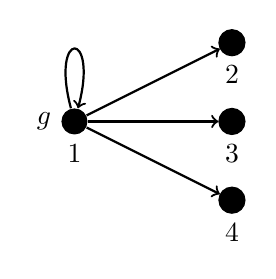
\begin{tikzpicture}
    \node[circle,fill,label={below:$1$},label={left:$g$}] (A) at (-1,0) {};
    \node[circle,fill,draw,label={below:$2$}] (B) at (1,1) {};
    \node[circle,fill,draw,label={below:$3$}] (C) at (1,0) {};
    \node[circle,fill,draw,label={below:$4$}] (D) at (1,-1) {};
    \draw[->,thick] (A) to[loop above,looseness=30] (A);
    \draw[->,thick] (A) -- (B);
    \draw[->,thick] (A) -- (C);
    \draw[->,thick] (A) -- (D);
\end{tikzpicture}
\hfill
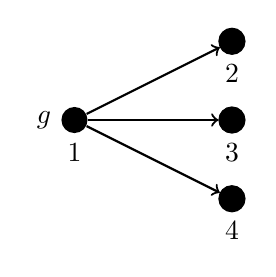
\begin{tikzpicture}
  \node[circle,fill,label={below:$1$},label={left:$g$}] (A) at (-1,0) {};
  \node[circle,fill,draw,label={below:$2$}] (B) at (1,1) {};
  \node[circle,fill,draw,label={below:$3$}] (C) at (1,0) {};
  \node[circle,fill,draw,label={below:$4$}] (D) at (1,-1) {};
  %\draw[->,thick] (A) to[loop above,looseness=30] (A);
  \draw[->,thick] (A) -- (B);
  \draw[->,thick] (A) -- (C);
  \draw[->,thick] (A) -- (D);
\end{tikzpicture}

Greta admires \hfill Greta admires\\
everyone. \hfill everyone \emph{else}.\\

\uncover<2->{\alert{$\forall x\, A(g,x)$}}\hfill\uncover<3->{\alert{$\forall x(\text{``$x$ is not Greta''} \eif A(g,x))$}}\\
\hfill\uncover<4->{\alert{$\forall x(\enot x= g \eif A(g,x))$}}

\end{frame}

\begin{frame}
  \frametitle{The identity predicate}

  \begin{itemize}[<+->]
    \item A new, special two-place predicate: \alert{$=$}
    \begin{itemize}[<+->]
      \item Written between arguments, \emph{without parentheses}.
      \item Needs no mention in symbolization key.
      \item Always interpreted the same: extension of $=$ is all pairs $\langle\alpha, \alpha\rangle$.
    \end{itemize}
    \item $a=b$ true iff $a$ and $b$ are names for one and the the same object.
    \item $x=y$ satisfied by all and only the pairs $\langle \alpha,\alpha\rangle$.
    \item $\lnot x=y$ is satisfied by a pair $\langle
    \alpha,\beta\rangle$ iff $\alpha$ and $\beta$ are different objects.
    \item \alert{$x = \lnot y$ is not grammatical.} \\
    ($\lnot$ can only go in front of a formula, and $y$ is not one.)
    \item \alert{$\lnot(x=y)$} is also not grammatical.\\
    ($(x=y)$ is also not a formula.)
  \end{itemize}
\end{frame}

\begin{frame}
    \frametitle{Something else/everything else}

\begin{itemize}[<+->]
\item Remember: different variables does not mean different objects.
\item $\exists x\exists y\,A(x,y)$ doesn't mean that someone admires
someone else.
\item It just means that someone admires someone (possibly
themselves).
\item To symbolize ``someone else'' add $\lnot x = y$:
\[\color{highlightA}
\exists x\exists y(\lnot x = y \land A(x,y))\]
\item $\forall x\forall y\,A(x,y)$ says that everyone admires everyone
(including themselves).
\item To symbolize ``everyone else'' add $\lnot x=y$:
\[\color{highlightA}
\forall x\forall y(\lnot x = y \eif A(x,y))\]
\end{itemize}
\end{frame}

\begin{frame}
  \frametitle{Something else/everything else}

\begin{itemize}[<+->]
\item The closest quantifier (typically) determines if you should use $\land$ or $\eif$:
\[
  \forall x\exists y(\lnot x = y \eand A(x,y)) \qquad
  \exists x\forall y(\lnot x = y \eif A(x,y))
\]
\item If you have mixed domains, it works the same way:
\item Everyone admires someone \emph{else}:
\[\color{highlightA}
\forall x(P(x) \eif \exists y((P(y) \eand \enot x = y) \eand A(x, y)))
\]
\item Someone admires everyone \emph{else}:
\[\color{highlightA}
\exists x(P(x) \eand \forall y((P(y) \eand \enot x = y) \eif A(x, y))
\]
\end{itemize}
\end{frame}

\begin{frame}
  \frametitle{Other than, except}
  
  
  \begin{itemize}[<+->]
    \item ``\emph{Someone other than Greta} is a hero'':
    \item[] \emph{$\exists x(\lnot x = g \eand H(x))$}
    \item ``\emph{Everyone other than Greta} is a hero'',
    \item ``\emph{Everyone except Greta} is a hero'':
    \item[] \emph{$\forall x(\lnot x = g \eif H(x))$}
    \end{itemize}
\end{frame}


\begin{frame}
  \frametitle{Singular ``only''}

  \begin{itemize}[<+->]
    \item ``\emph{No-one other than Greta} is a hero'':
    \item[] \emph{$\enot\exists x(H(x) \eand \enot x = g)$}
    \item[] \emph{$\forall x(H(x) \eif x = g)$}
    \item ``\emph{Only Greta} is a hero'':
    \item No-one other than Greta is a hero, and Greta is a hero:
    \item[] \emph{$\forall x(H(x) \eif x = g) \eand H(g)$}
    \item[] \emph{$\forall x(H(x) \eiff x = g))$}
  \end{itemize}
  \end{frame}
  
\begin{frame}
    \frametitle{Uniqueness}

\begin{itemize}[<+->]
\item There is at least one hero.
\[\color{highlightA}
\exists x\, H(x)
\]
\item There is exactly one hero.
\begin{itemize}[<+->]
\item There's at least one hero, and
\item There are no others:
\begin{align*}
\uncover<5->{\exists x\, (H(x) \land {}} & 
  \uncover<6->{\textcolor{highlightA}{\lnot \exists y\, (\lnot y = x \land H(y)))}}\\
\uncover<7->{\exists x\,(H(x) \land {}} & 
\uncover<7->{\textcolor{highlightA}{\forall y(H(y) \to x = y))}}
\end{align*}
\item<8>Or more succinctly: 
$\color{highlightA}\exists x\forall y(H(y) \eiff x=y)$
\end{itemize}
\end{itemize}
\end{frame}


\subsection{Numerical quantification}

\begin{frame}
    \frametitle{Numerical Quantification}

\begin{itemize}[<+->]
\item Cardinal numbers can be determiners:
\begin{itemize}
\item \emph{Three heroes} wear capes.
\end{itemize}
\item Not always clear if ``three heroes'' means \emph{exactly} or \emph{at least} three.
\item We'll assume the latter.%---the ``exactly'' is implicated, not implied. Why?
\begin{itemize}[<+->]
\item Do you have two dollars? Yes, I have two dollars. \\ (Uncontroversially true even if you have more than 2\$)
%\item How much money do you have? I have two dollars. \\ (True but misleading if you have more.)
\end{itemize}
\item FOL can express all of:
\begin{itemize}[<+->]
\item \emph{At least $n$} people are \dots
\item \emph{Exactly $n$} people are \dots
\item \emph{At most $n$} people are \dots
\end{itemize}
\end{itemize}
\end{frame}

\begin{frame}
    \frametitle{At least $n$}

\begin{itemize}[<+->]
\item At least 1 hero is inspiring:
\[
\alert{\exists x(H(x) \land I(x))}
\]
\item At least 2 heroes are inspiring:
\[
\alert{\exists x\exists y(\enot x = y \land ((H(x) \land I(x)) \land (H(y) \land I(y))))}
\]
\item At least 3 heroes are inspiring:
\begin{align*}
& \alert{\exists x\exists y\exists z((\enot x = y \land (\enot y = z \land \enot x = z)) \eand {}} \\
& \qquad \alert{((H(x) \land I(x)) \land ((H(y) \land I(y)) \eand (H(z) \land I(z))))}
\end{align*}
\end{itemize}
\end{frame}


\begin{frame}
  \frametitle{At least $n$}

\begin{itemize}
\item There are at least $n$ $A$s (``$\exists^{\ge n} x\,A(x)$'')::
\begin{align*}
\exists x_1\dots\exists x_n\uncover<2->{((\enot x_1 = x_2 \land (\enot x_1 = x_3 \land \dots \land (\enot x_1 = x_n} & \uncover<2->{{} \land {}}\\
\uncover<2->{(\enot x_2 = x_3 \land \dots \land (\enot x_2 = x_n} & \uncover<2->{{} \land {}}\\
\uncover<2->{\ddots}\qquad &\\
\uncover<2->{\enot x_{n-1} = x_n)\dots)} & \uncover<2->{{} \land {}}\\
\uncover<3->{(A(x_1) \land (A(x_2) \land \dots \land A(x_n))\dots))}
\end{align*}
\end{itemize}
\end{frame}

\begin{frame}
  \frametitle{At least $n$}

\begin{itemize}[<+->]
\item Note: must state that \emph{every pair} of variables is different, e.g.,
\begin{align*}
\exists x_1\exists x_2\exists x_3(&(\enot x_1 = x_2 \land \enot x_2 = x_3) \land {}\\
& (H(x_1) \land (H(x_2) \land H(x_3))))
\end{align*}
only says ``There are at least two heroes''!
\begin{itemize}[<+->]
  \item Take extension of $H(x)$ to be: $1,2$
  \item Then $1$ can play role of $x_1$ and $x_3$, $2$ role of $x_2$.
  \item Both ``$\enot 1=2$'' and ``$\enot 2=3$'' are true.
\end{itemize}
\item At least $n$ $B$s are $C$s: take $B(x) \eand C(x)$ for $A(x)$:
\[
\exists^{\ge n} x(B(x) \land C(x))
\]
\end{itemize}
\end{frame}

\begin{frame}
    \frametitle{Exactly one}

\begin{itemize}[<+->]
\item There is exactly one hero:
\[
\exists x(H(x) \land \lnot \exists y(H(y) \land \enot x = y))
\]
\item This is equivalent to:
\[
\exists x(H(x) \land \forall y(H(y) \to x = y))
\]
\item In general: ``$x$ has property $A$ \emph{uniquely}'':
\begin{align*}
A(x) \land {} & \forall y(A(y) \to x = y)\\
\text{or just:\qquad} & \forall y(A(y) \eiff x = y)
\end{align*}
\end{itemize}
\end{frame}

\begin{frame}
  \frametitle{Exactly $n$}

\begin{itemize}
\item<1-> There are exactly $n$ $A$s (``$\exists^{=n} x\,A(x)$''):
\begin{align*}
\exists x_1\dots\exists x_n\uncover<2->{((\enot x_1 = x_2 \land (\enot x_1 = x_3 \land \dots \land (\enot x_1 = x_n} & \uncover<2->{{} \land {}}\\
\uncover<2->{(\enot x_2 = x_3 \land \dots \land (\enot x_2 = x_n} & \uncover<2->{{} \land {}}\\
\uncover<2->{\ddots}\qquad &\\
\uncover<2->{\enot x_{n-1} = x_n)\dots)} & \uncover<3->{{} \land {}}\\
\uncover<presentation:3-4|handout:1>{(A(x_1) \land (A(x_2) \land \dots \land A(x_n))\dots))} & \uncover<presentation:4|handout:1>{{} \eand {}}\\
\uncover<4->{\forall y(A(y) \only<presentation: 4|handout:1>{\eif} \only<presentation: 5-|handout:2>{\eiff} (y = x_1 \lor \dots \lor y=x_n)))}
\end{align*}
\item<6-> Exactly $n$ $B$s are $C$s:
\[
\exists^{=n}x (B(x) \land C(x))
\]
\end{itemize}
\end{frame}

\begin{frame}
    \frametitle{At most $n$}

\begin{itemize}
\item<1-> There are \emph{at most $n$} As $\Leftrightarrow$ There are
\emph{not at least $n+1$} As
\[
\exists^{\alert{\le n}}x\, A(x) \Leftrightarrow \alert{\lnot}\exists^{\alert{\ge(n+1)}}x\, A(x)
\]
\item<2-> For instance: There are at most two heroes:
\begin{align*}
\uncover<2->{\lnot \exists x\exists y\exists z((H(x) \land (H(y) \land H(z)))}
& \uncover<2->{\land (\lnot x =y \land (\lnot x = z \land \lnot y = z)) )}\\
\uncover<3->{\forall x\forall y\forall z((H(x) \land (H(y) \land H(z)))
} &\uncover<3->{\eif (x =y \lor ( x = z \lor y = z)) )}
\end{align*}
\item<4-> $\lnot\exists^{\ge(n+1)}x\, A(x)$ is equivalent to:
\begin{align*}
\forall x_1\dots\forall x_{n+1} ((A(x_1) \land \dots \land A(x_{n+1})) \eif \qquad \\
(x_1 = x_2 \lor (x_1 = x_3 \lor \dots \lor (x_1 = x_{n+1} & {} \lor {}\\
(x_2 = x_3 \lor \dots \lor (x_2 = x_{n+1} & {} \lor {}\\
\ddots\qquad &\\
x_n = x_{n+1})\dots) & ))
\end{align*}
\end{itemize}
\end{frame}

\newhourlecture

\subsection{``The'', ``both'', ``neither''}

\begin{frame}
    \frametitle{Definite descriptions}

\begin{itemize}[<+->]
\item Definite description: \emph{the so-and-so}
\item Russell's analysis of definite description: to say\\
\begin{itemize}[<+->]
\item ``The $A$ is B''\\
\end{itemize}
is to say:
\begin{itemize}[<+->]
\item There is a unique $A$
\item It is $B$
\end{itemize}
\item In FOL:
\[
\exists x(A(x) \land \forall y(A(y) \to x = y) \land B(x))
\]
\item or more succinctly:
\[
\exists x(\forall y(A(y) \eiff x = y) \land B(x))
\]
\end{itemize}
\end{frame}

\begin{frame}
\frametitle{``The'' vs. ``exactly one''}

\begin{itemize}[<+->]
\item Compare:
\begin{enumerate}[<+->]
\item The hero inspires:
\[\exists x(H(x) \land \forall y(H(y) \to x = y) \land I(x))\]
\item There is exactly one inspiring hero:
\[\exists x(H(x) \land \forall y((H(y) \alert{{}\land I(y)}) \to x = y) \land I(x))\]
\end{enumerate}
\item (2) can be true without (1), but not vice versa.
\item (Namely when there is exactly one inspiring hero, but also a non-inspiring hero.)
\item So (1) entails (2), but not vice versa.
\end{itemize}
\end{frame}

\begin{frame}
    \frametitle{Strawson's analysis}

\begin{itemize}
\item According to Russell, ``The hero wears a cape'' is false if there is no hero, or if there is more than one.
\item P. F. Strawson disagrees: we only succeed in making a statement
if there is a unique hero.
\item ``There is a unique hero'' is not part of what is \emph{said}, but is only \emph{presupposed}.
\end{itemize}
\end{frame}

\begin{frame}
  \frametitle{Singular possessive}

  \begin{itemize}[<+->]
    \item Singular possessives make noun phrases, e.g., ``Joe's cape''
    \item They work like definite descriptions: Joe's cape is the cape Joe owns.
    E.g.:
    \begin{itemize}
      \item ``Autumn wears \alert{Joe's cape}'' symbolizes the same as:
      \item[] ``Autumn wears \alert{the cape Joe owns}'':
      \item[]
      \begin{align*}
        \exists x[& \uncover<6->{((E(x) \land O(d,x)) \land {}}\\
        & \uncover<7->{\forall y((E(y) \land O(d,y)) \eif x=y)) \land {}}\\
        & \uncover<8->{W(a,x)]}
      \end{align*}
    \end{itemize}
  \end{itemize}
\end{frame}

\begin{frame}
  \frametitle{Singular vs. plural possessive}

  \begin{itemize}[<+->]
    \item Compare \emph{plural} possessives: those are $\forall$'s:
    \begin{itemize}[<+->]
      \item ``Autumn wears \alert{Joe's cape\textbf{s}}'' symbolizes the same
      as:
      \item[] ``Autumn wears every cape that Joe owns'':
      \[\forall x[(E(x) \land O(d,x)) \eif W(a,x)]\]
    \end{itemize}
  \end{itemize}
\end{frame}

\begin{frame}
    \frametitle{Both}

\begin{itemize}
\item<1-> ``Both heroes inspire'': There are exactly 2 heroes, and both inspire:
\begin{align*}
\exists x\exists y\uncover<2->{[((\enot x = y \land (H(x) \land H(y)))} & 
\uncover<3->{{} \land {}}\\
\uncover<3->{\forall z(H(z) \to (z = x \lor z = y)))} & \uncover<4->{{}\land {}}\\
\uncover<4->{(I(x) \eand I(y))]}&
\end{align*}
\item<5-> Note: ``Both heroes inspire'' implies ``There are exactly two inspiring heroes'', but not vice versa!
\end{itemize}
\end{frame}

\begin{frame}
    \frametitle{Neither}

\begin{itemize}[<+->]
\item ``Neither hero inspires'': There are exactly 2 heroes, and neither of them inspires:
\begin{align*}
\exists x\exists y[((\lnot x = y \land (H(x) \land H(y))) & {}\land {}\\
\forall z(H(z) \to (z = x \lor z = y))) &{} \land {}\\
(\enot I(x) \eand \enot I(y))]&
\end{align*}
\end{itemize}
\end{frame}


\newhourlecture
\newonlinelecture

\section{Proofs for full FOL}

\subsection{Proofs with multiple quantifiers}

\begin{frame}
  \frametitle{Eliminating $\forall$}

  \begin{fitchproof}
    \have[m]{a}{\forall \metav{x}\metav{A}(\ldots \metav{x} \ldots \metav{c}\ldots)}
    \have[\ ]{c}{\metav{A}(\ldots \metav{c} \ldots \metav{c}\ldots)} \Ae{a}
  \end{fitchproof}
  \begin{itemize}
    \item No restriction on $\metav{c}$:
    \begin{itemize}[<+->]
      \item May be in an assumption.
      \item May also be in $\forall \metav{x}\metav{A}(\ldots \metav{x}
      \ldots \metav{x}\ldots)$ already!
    \end{itemize}
  \end{itemize}
\end{frame}

\begin{frame}{Working forward from $\forall$}

  \begin{itemize}[<+->]
    \item If you \emph{have $\forall \metav{x}\metav{A}(\metav{x})$}, replace every $\metav{x}$ by the
      same $\metav{c}$.
    \item The result is $\metav{A}(\metav{c})$, justified by $\forall E$.
    \item You can pick any $\metav{c}$.
    \item Good candidates: $\metav{c}$ which occur in assumptions or
      in the sentences you're trying to prove.
    \item You may need to try multiple candidates.
    \end{itemize}
\end{frame}

\begin{frame}
  \frametitle{Introducing $\forall$}
  
  \begin{fitchproof}
    \have[m]{a}{\metav{A}(\ldots \metav{c} \ldots \metav{c}\ldots)}
    \have[\ ]{c}{\forall \metav{x}\metav{A}(\ldots \metav{x} \ldots \metav{x}\ldots)} \Ai{a}
  \end{fitchproof}

  \begin{itemize}[<+->]
  \item Restrictions on $\metav{c}$:
  \begin{itemize}
    \item must not occur in any undischarged assumption.
    \item must not occur in $\forall \metav{x}\metav{A}(\ldots \metav{x} \ldots \metav{x})$.
  \end{itemize}
\end{itemize}
\end{frame}

\begin{frame}{Working backward from $\forall$}

  \begin{itemize}[<+->]
    \item If you \emph{want $\forall \metav{x}\metav{A}(\metav{x})$}, replace every $\metav{x}$ by the
      same $\metav{c}$.
    \item The result is $\metav{A}(\metav{c})$. 
    \item Try to prove this \emph{above} $\forall \metav{x}\metav{A}(\metav{x})$.
    \item Justify $\forall \metav{x}\metav{A}(\metav{x})$ by $\forall I$.
    \item You must pick a \emph{new} $\metav{c}$ not already in the
    proof constructed so far.
    \item As long as $\metav{c}$ is fresh, this will work if you can
    prove $\forall \metav{x}\metav{A}(\metav{x})$ at all.
    \end{itemize}
\end{frame}


\begin{frame}
  \frametitle{Introducing $\exists$}

  \begin{fitchproof}
    \have[m]{a}{\metav{A}(\ldots \metav{c} \ldots \metav{c}\ldots)}
    \have[\ ]{c}{\exists \metav{x}\metav{A}(\ldots \metav{x} \ldots \metav{c}\ldots)}\Ei{a}
  \end{fitchproof}
  \begin{itemize}[<+->]
    \item No restriction on $\metav{c}$:
    \begin{itemize}[<+->]
      \item May be in an assumption.
      \item May also be in $\exists \metav{x}\metav{A}(\ldots \metav{x}
      \ldots \metav{c}\ldots)$.
      \item So you can also justify $\exists \metav{x}\metav{A}(\ldots \metav{x}
      \ldots \metav{x}\ldots)$ or $\exists \metav{x}\metav{A}(\ldots \metav{c}
      \ldots \metav{x}\ldots)$.
    \end{itemize}
  \end{itemize}
\end{frame}

\begin{frame}{Working backward from $\exists$}

  \begin{itemize}[<+->]
    \item If you \emph{want} $\exists \metav{x}\metav{A}(\metav{x})$, replace every $\metav{x}$ by the
      same $\metav{c}$.
    \item The result is $\metav{A}(\metav{c})$. 
    \item Try to prove this \emph{above} $\exists \metav{x}\metav{A}(\metav{x})$
    \item Justify $\exists \metav{x}\metav{A}(\metav{x})$ by $\exists I$.
    \item You can pick any $\metav{c}$.
    \item Good candidates: $\metav{c}$ which occur in assumptions or
      in the sentences you're trying to prove.
    \item That includes $\exists \metav{x}\metav{A}(\metav{x})$!
    \item You may need to try multiple candidates.
    \item This may not work (especially at the beginning, or if
    you need~IP)!
    \item Try other strategies first, especially strategies that put
    more $\metav{c}$ into play ($\exists E$).
    \end{itemize}
\end{frame}

\begin{frame}
  \frametitle{Eliminating $\exists$}
  \begin{fitchproof}
    \have[m]{a}{\exists \metav{x}\metav{A}(\ldots \metav{x} \ldots \metav{x}\ldots)}
    \open
      \hypo[i]{b}{\metav{A}(\ldots \metav{c} \ldots \metav{c}\ldots)}
      \have[j]{c}{\metav{B}}
    \close
    \have[\ ]{d}{\metav{B}}\Ee{a,b-c}
  \end{fitchproof}

  \begin{itemize}[<+->]
    \item Restrictions on $\metav{c}$:
    \begin{itemize}[<+->]
      \item must not occur in any assumption still open when you apply
      $\exists E$.
      \item must not occur in $\exists \metav{x}\metav{A}(\ldots \metav{x} \ldots \metav{x}$).
      \item must not occur in $\metav{B}$.
    \end{itemize}
  \end{itemize}
  \end{frame}

  \begin{frame}{Working forward from $\exists$}

  \begin{itemize}[<+->]
    \item If you \emph{have $\exists \metav{x}\metav{A}(\metav{x})$}, and you \emph{want  $\metav{B}$}:
      \begin{itemize}
        \item replace every $\metav{x}$ by the
        same $\metav{c}$.
        \item The result is $\metav{A}(\metav{c})$.
        \item Start a subproof with this.
        \item Prove $\metav{B}$ on its last line
        \item Justify $\metav{B}$ after the subproof using $\exists E$.
        \end{itemize}
    \item You must pick a \emph{new} $\metav{c}$ not already in the
    proof constructed so far.
    \item As long as $\metav{c}$ is fresh, this will work if you can
    prove $\metav{B}$ from $\exists \metav{x}\metav{A}(\metav{x})$ at all.
    \end{itemize}
\end{frame}

\begin{frame}
    \frametitle{Admirers and admired}

\begin{earg}
\item[] Someone is admired by everyone
\item[\therefore] Everyone admires someone
\end{earg}

\bigskip
\begin{fitchproof}
\hypo[ ]{1}{\exists y\forall x\, A(x, y)}
\have[ ]{2}{\forall x\exists y\, A(x, y)}
\end{fitchproof}
Let's do it on \href{https://carnap.io/shared/rzach@ucalgary.ca/Practice\%20Problems\%20VII.md}{carnap.io}
\end{frame}

\begin{frame}
  \frametitle{Admirers and admired}

  \begin{fitchproof}
    \hypo{1}{\exists y\forall x\, A(x, y)}
    \open
    \hypo{2}{\forall x\,A(x, c)}
    \have{3}{A(d,c)}\Ae{2}
    \have{4}{\exists y\,A(d,y)}\Ei{3}
    \have{5}{\forall x\exists y\,A(x,y)}\Ai{4}
    \close
    \have{6}{\forall x\exists y\, A(x, y)}\Ee{1,2-5}
  \end{fitchproof}
\end{frame}

\begin{frame}
    \frametitle{All hail Queen Anne}

\begin{earg}
\item[] Some woman is superior to every man.
\item[\therefore] Every man is inferior to some woman.
\end{earg}

\bigskip

\begin{fitchproof}
\hypo[ ]{1}{\exists y(W(y) \land \forall x(M(x) \to S(y, x)))}
\have[ ]{2}{\forall x(M(x) \to \exists y(W(y) \land S(y, x)))}
\end{fitchproof}
\end{frame}

\begin{frame}\footnotesize

\begin{fitchproof}
\hypo{1}{\exists y(W(y) \land \forall x(M(x) \to S(y, x)))}
\open
\hypo{2}{W(c) \land \forall x(M(x) \to S(c, x))}
\open
\hypo{3}{M(d)}
\have{4}{\forall x(M(x) \to S(c, x))}\ae{2}
\have{5}{M(d) \to S(c, d))}
\have{6}{S(c,d)}
\have{7}{W(c)}\ae{2}
\have{8}{W(c) \land S(c,d)}\ai{6,7}
\have{9}{\exists y(W(y) \land S(y, x))}\Ei{8}
\close
\have{10}{M(d) \to \exists y(W(y) \land S(y, d))}
\have{11}{\forall x(M(x) \to \exists y(W(y) \land S(y, x)))}\Ai{10}
\close
\have{12}{\forall x(M(x) \to \exists y(W(y) \land S(y, x)))}\Ee{1,2-11}
\end{fitchproof}
\end{frame}

\subsection{Proofs with identity}

\begin{frame}
    \frametitle{Everybody loves my baby}


\begin{earg}
\item[] Everybody loves my baby.
\item[] But my baby don't love nobody but me.
\item[\therefore] My baby is me.
\end{earg}

\bigskip

\begin{fitchproof}
\hypo[ ]{1}{\forall x\, L(x, b)}
\hypo[ ]{2}{\forall x(L(b, x) \eif x = i)}
\have[ ]{3}{b = i}
\end{fitchproof}

\small\begin{itemize}
\item
\href{https://www.youtube.com/results?search_query=\%22Everybody+loves+my+baby\%22}{``Everybody
Loves my Baby'' on YouTube}
\end{itemize}

\end{frame}

\begin{frame}
  \frametitle{My baby is me}

  \begin{fitchproof}
\hypo{1}{\forall x\, L(x, b)}
\hypo{2}{\forall x(L(b, x) \eif x = i)}
\have{3}{L(b,b)}\Ae{1}
\have{4}{L(b,b) \eif b = i}\Ae{2}
\have{5}{b = i}\ce{3,4}
\end{fitchproof}
\end{frame}

\begin{frame}
  \frametitle{I am my baby}

  \begin{fitchproof}
\hypo{1}{\forall x\, L(x, b)}
\hypo{2}{\forall x(L(b, x) \eif x = i)}
\have{3}{L(b,b)}\Ae{1}
\have{4}{L(b,b) \eif b = i}\Ae{2}
\have{5}{i = b}\by{?}{}
\end{fitchproof}
\end{frame}

\begin{frame}
  \frametitle{Proofs with identity}
  
  \begin{fitchproof}
    \have[\ \,\,\,]{x}{\metav{c}=\metav{c}} \by{=I}{}
  \end{fitchproof}
  
  \begin{fitchproof}
    \have[m]{e}{\metav{a}=\metav{b}}
    \have[n]{a}{\metav{A}(\ldots \metav{a} \ldots \metav{a}\ldots)}
    \have[\ ]{ea1}{\metav{A}(\ldots \metav{b} \ldots \metav{a}\ldots)} \by{=E}{e,a}
  \end{fitchproof}
  \begin{fitchproof}
    \have[m]{e}{\metav{a}=\metav{b}}
    \have[n]{a}{\metav{A}(\ldots \metav{b} \ldots \metav{b}\ldots)}
    \have[\ ]{ea2}{\metav{A}(\ldots \metav{a} \ldots \metav{b}\ldots)} \by{=E}{e,a}
  \end{fitchproof}
\end{frame}

\begin{frame}
  \frametitle{I am my baby}

  \begin{itemize}
    \item We symbolized ``My baby is me'' as $b = i$.
    \item But it's equivalent to ``I am my baby,'' $i = b$.
    \item $=$I and $=$E let us prove this:
    \begin{fitchproof}
      \hypo{1}{b = i}
      \have{2}{b = b}\by{=I}{}
      \have{3}{i = b}\by{=E}{1,2}
    \end{fitchproof}
  \end{itemize}
\end{frame}

\begin{frame}
  \frametitle{Different properties, different things}

  \begin{itemize}[<+->]
    \item Two names $d$, $e$ may name the same thing.
    \item In that case, $d = e$ would be true.
    \item And then anything that's true about $d$ is also true about $e$.
    \item In other words: \[d=e,P(d) \models P(e)\]
    \item So if something is true about $d$ but false about $e$, then $\enot d = e$. 
    \item In other words:
    \[P(d), \enot P(e) \models \enot d = e\]
  \end{itemize}
\end{frame}

\begin{frame}
  \frametitle{Different properties, different things}

  \begin{fitchproof}
    \hypo{1}{P(d)}
    \hypo{2}{\enot P(e)}
    \open
    \hypo{3}{d = e}
    \have{4}{P(e)}\by{=E}{1,3}
    \have{5}{\ered}\ne{2,4}
    \close
    \have{6}{\enot d = e}\ni{2-5}
  \end{fitchproof}
\end{frame}

\begin{frame}
  \frametitle{Uniqueness, again}

  The two symbolizations  of ``there is exactly one hero'' are equivalent:
  \begin{align*}
    \exists x&(H(x) \land \forall y(H(y) \to x = y))\\
    \exists x\forall y & (H(y) \eiff x=y)
  \end{align*}
\end{frame}

\begin{frame}
  \frametitle{Uniqueness, again}
  \tiny
  \begin{fitchproof}
    \hypo{1}{\exists x(H(x) \land \forall y(H(y) \to x = y))}
    \open
    \hypo{2}{H(a) \land \forall y(H(y) \to a = y)}
    \open
    \hypo{3}{H(c)}
    \have{4}{\forall y(H(y) \to a = y)}\ae{2}
    \have{5}{H(c) \to a = c}\Ae{4}
    \have{6}{a=c}\ce{3,5}
    \close
    \open
    \hypo{7}{a=c}
    \have{8}{H(a)}\ae{2}
    \have{9}{H(c)}\ie{7,8}
    \close
    \have{10}{H(c) \eiff a=c}\bi{3-6,7-9}
    \have{11}{\forall y  (H(y) \eiff a=y)}\Ai{10}
    \have{12}{\exists x\forall y  (H(y) \eiff x=y)}\Ei{11}
    \close
    \have{13}{\exists x\forall y  (H(y) \eiff x=y)}\Ee{1,2-12}
  \end{fitchproof}
\end{frame}

\begin{frame}
  \frametitle{Uniqueness, again}
\tiny
  \begin{fitchproof}
    \hypo{1}{\exists x\forall y  (H(y) \eiff x=y)}
    \open
    \hypo{2}{\forall y (H(y) \eiff a=y)}
    \have{4}{H(a) \eiff a = a}\Ae{2}
    \have{5}{a = a}\ii{}
    \have{6}{H(a)}\be{4,5}
    \open
    \hypo{7}{H(c)}
    \have{8}{H(c) \eiff a = c}\Ae{2}
    \have{9}{a=c}\be{7,8}
    \close
    \have{10}{H(c) \eif a=c}\ci{7-9}
    \have{11}{\forall y(H(y) \to a = y)}\Ai{10}
    \have{12}{H(a) \land \forall y(H(y) \to a = y)}\ai{6,11}
    \have{13}{\exists x(H(x) \land \forall y(H(y) \to x = y))}\Ei{12}
    \close
    \have{14}{\exists x(H(x) \land \forall y(H(y) \to x = y))}\Ee{1,2-13}
  \end{fitchproof}
\end{frame}

\newhourlecture

\begin{frame}
    \frametitle{Proofs with numerical claims}

\begin{fitchproof}
\hypo[ ]{1}{\exists x\, P(x)}
\hypo[ ]{2}{\forall x\forall y ((P(x) \land P(y)) \to x = y)}
\have[ ]{3}{\exists x(P(x) \land \forall y(P(y) \to x = y))}
\end{fitchproof}
\end{frame}

\begin{frame}
  \frametitle{Proofs with numerical claims}
\tiny
\begin{fitchproof}
\hypo{1}{\exists x\, P(x)}
\hypo{2}{\forall x\forall y ((P(x) \land P(y)) \to x = y)}
\open
\hypo{3}{P(a)}
\open
\hypo{4}{P(c)}
\have{5}{\forall y ((P(a) \land P(y)) \to a = y)}\Ae{2}
\have{6}{(P(a) \land P(c)) \to a = c}\Ae{5}
\have{7}{P(a) \land P(c)}\ai{3,4}
\have{8}{a=c}\ce{6,7}
\close
\have{9}{P(c) \eif a=c}\ci{4-8}
\have{10}{\forall y(P(y) \to a = y)}
\have{11}{P(a) \land \forall y(P(y) \to a = y)}\ai{3,11}
\have{12}{\exists x(P(x) \land \forall y(P(y) \to x = y))}\Ei{11}
\close
\have{13}{\exists x(P(x) \land \forall y(P(y) \to x = y))}\Ee{1,3-12}
\end{fitchproof}
\end{frame}


\newhourlecture
\newonlinelecture

\section{Interpretations for full FOL}



\begin{frame}
  \frametitle{Converses are invalid}

  \[
    \forall x\exists y\, A(x, y) \not\models \exists y\forall x\, A(x, y)
\]
\[
    \forall x(M(x) \to \exists y(W(y) \land S(y, x)))
    \not\models \exists y(W(y) \land \forall x(M(x) \to S(y, x)))
\]

  Let's do it on \href{https://carnap.io/shared/rzach@ucalgary.ca/Practice\%20Problems\%20VI.md}{carnap.io}
\end{frame}

\newhourlecture
\newonlinelecture

\section{Expressive adequacy and normal forms}

\subsection{Functional completeness}

\begin{frame}
    \frametitle{Truth functions}

\begin{block}{Definition}

An ($n$-place) \emph{truth function} $t$ is a mapping of $n$-tuples of \True{} and \False\ to either \True\ or \False.
\medskip

$n$-place truth functions correspond to truth tables of sentence $S$ with $n$ sentence letters $A_1$, \dots, $A_n$.
\end{block}

\begin{columns}
  \begin{column}{.5\textwidth}
$\begin{array}{cc|cc}
\uncover<2->{A_1} & \uncover<2->{A_2} & t_\land & 
\only<2>{S}\only<3-4>{A_1 \land A_2}\\ \hline
\True & \True & \True & \only<2>{?}\only<3->{\True} \\
\True & \False & \False & \only<2>{?}\only<3->{\False}\\
\False & \True & \False & \only<2>{?}\only<3->{\False}\\
\False & \False & \False & \only<2>{?}\only<3->{\False}
\end{array}$
\end{column}
\begin{column}{.5\textwidth}
$\begin{array}{cc|cc}
  \uncover<2->{A_1} & \uncover<2->{A_2} & t_\lor & 
  \only<2-3>{S}\only<4>{A_1 \lor A_2}\\ \hline
\True & \True & \True & \only<2-3>{?}\only<4>{\True}\\
\True & \False & \True & \only<2-3>{?}\only<4>{\True}\\
\False & \True & \True & \only<2-3>{?}\only<4>{\True}\\
\False & \False & \False & \only<2-3>{?}\only<4>{\False}
\end{array}$
\end{column}
\end{columns}

\end{frame}

\begin{frame}
    \frametitle{Truth functions}

\begin{block}{Definition}
A sentence $S$ containing the sentence letters $A_1$, \dots, $A_n$
\emph{expresses} the truth function $t$ iff the truth value of $S$ on
the valuation which assigns $v_i$ to $A_i$ is $t(v_1,
\dots, v_n)$.
\medskip

An $n$-place truth function is \emph{expressible} if there is a
sentence containing sentence letters $A_1$, \dots, $A_n$ that
expresses it.
\end{block}
\end{frame}


\begin{frame}
    \frametitle{Examples}

\begin{tabular}{cc}
$\begin{array}{cc|cl}
  \uncover<2->{A_1} & \uncover<2->{A_2} & t_1 & \uncover<2->{S?}\\ \hline
\True & \True & \True \\
\True & \False & \True \\
\False & \True & \False \\
\False & \False & \False
\end{array}$
& \uncover<3->{$A_1 \quad\text{or:}\quad A_1 \land (A_2 \lor \lnot A_2)$} \\ \ \\
$\begin{array}{cc|cl}
  \uncover<2->{A_1} & \uncover<2->{A_2} & t_\mathit{xor} &\uncover<2->{S?}\\ \hline
\True & \True & \False \\
\True & \False & \True \\
\False & \True & \True \\
\False & \False & \False
\end{array}$
&
\uncover<4->{$(A_1 \lor A_2) \land \lnot(A_1 \land A_2)$ or: $\enot (A_1 \eiff A_2)$}
\end{tabular}
\end{frame}

\begin{frame}
  \frametitle{Functional completeness}

  \begin{block}{Definition}
  A collection of connectives is \emph{functionally complete} if every
  truth function is expressible by a sentence containing only those
  connectives.
  \end{block}

\end{frame}

\begin{frame}
  \frametitle{Functional completeness: results}

\begin{itemize}[<+->]
  \item Functionally complete are:
  \begin{itemize}[<+->]
  \item Connectives we know:
  \[
    {\alert{\eand}} + {\alert{\enot}} \qquad 
  {\alert{\lor}} +
  {\alert{\enot}} \qquad 
  {\alert{\eif}} +
  {\alert{\enot}} \qquad {\alert{\eif}} +
  {\alert{\bot}}\] 
  \item Any other set of connectives containing one of those.
  \item Two two-place connectives by themselves: neither--not (\textsc{nor}) and not--both (\textsc{nand}).
  \end{itemize}
  \item No other (sets of) one and two-place connectives are functionally complete.
  \item We'll prove this for $\eand + \eor$.
\end{itemize}
\end{frame}

\subsection{Proving connectives aren't functionally complete}

\begin{frame}
  \frametitle{$\land + \lor$ not functionally complete}

\begin{itemize}[<+->]
\item $\eand + \lor$ is not functionally complete.
\item Remember: To be functionally complete, \emph{every} truth
  function would have to be expressible using only $\eand$ and $\eor$.
\item Which 2-place truth-functions can be expressed using $\eand$ and
  $\eor$?
\item Not this one:
\[
\begin{array}{cc|c}
  && t_{\mathit{xor}}\\ \hline
\True & \True & \False \\
\True & \False & \True \\
\False & \True & \True \\
\False & \False & \False
\end{array}
\]
\end{itemize}
\end{frame}

\begin{frame}
    \frametitle{Proof by induction}

\begin{itemize}[<+->]
\item Sometimes need to prove something for \emph{all} sentences.
\item E.g., ``every sentence containing only $\land$ and $\lor$ expresses a truth function \emph{other than} $t_\mathit{xor}$.''
\item Proof by \emph{induction}:
\begin{itemize}[<+->]
\item Show that it holds for \emph{sentence letters} (and $\bot$).
\item Suppose sentences \emph{$\metav{P}$}, \emph{$\metav{Q}$} have the property.
\item Now show that it then also holds for \emph{$(\metav{P} \land \metav{Q})$}, \emph{$(\metav{P} \lor \metav{Q})$}, etc.
\end{itemize}
\item Why does this work? 
\item This is how we form sentences (involving only $\land$, $\lor$).
\item Property ``$S$ is a sentence expressing a truth function other than~$t_\mathit{xor}$'' propagates from atomic sentences to all sentences.
\end{itemize}
\end{frame}

\begin{frame}
    \frametitle{Proof by induction: example}

\begin{theorem}
Every sentence contains an even number of parentheses.
\end{theorem}

\begin{itemize}[<+->]
\item Every atomic sentence contains an even number of parentheses:
\[
B \qquad \bot
\]
\item If $\metav{P}$ contains an even number of parentheses, so does $\lnot \metav{P}.$
\item If $\metav{P}$ and $\metav{Q}$ both contain an even number of parentheses, so do
\[ (\metav{P} \land \metav{Q}), (\metav{P} \lor \metav{Q}), (\metav{P} \eif \metav{Q}), (\metav{P} \eiff \metav{Q}). \]
\end{itemize}
\end{frame}

\begin{frame}
  \frametitle{$\land + \lor$ not functionally complete}

\begin{theorem}
Any sentence containing only $A_1$, $A_2$, $\land$, $\lor$
has a $\True$ in the first line of its truth table.
\end{theorem}

\begin{itemize}[<+->]
\item Sentence letters: truth table of $A_i$ is just copy of column under $A_i$, so has $\True$ in first line where valuation assigns $\True$ to $A$.  
\item Suppose $\metav{P}$, $\metav{Q}$ are sentences which
  contain only $A_1$, $A_2$, $\land$, $\lor$ and are true in first line.
\item $(\metav{P} \land \metav{Q})$ is true in first line, since $\True \land \True$ makes $\True$.
\item $(\metav{P} \lor \metav{Q})$ is true in first line, since $\True
\lor \True$ makes $\True$.
\end{itemize}
\end{frame}

\begin{frame}
  \frametitle{$\land + \lor$ not functionally complete}

\begin{theorem}
Any sentence containing only $A_1$, $A_2$, $\land$, $\lor$
  expresses a truth function $t$ with $t(\True, \True) = \True$.
\end{theorem}

\begin{itemize}[<+->]
\item Sentence letters: $A_1$, $A_2$: express $t_1$, $t_2$.
\item Suppose $\metav{P}$, $\metav{Q}$ are sentences which
  contain only $A_1$, $A_2$, $\land$, $\lor$ and express truth
  functions $t$, $t'$ with $t(\True, \True) = t'(\True, \True) = \True$
\item $(\metav{P} \land \metav{Q})$ expresses truth function $s$ with
\[s(\True, \True) = t_\land(t(\True, \True), t'(\True, \True)) = \True\]
\item $(\metav{P} \lor \metav{Q})$ expresses truth function $s$ with
\[s(\True, \True) = t_\lor(t(\True, \True), t'(\True, \True)) = \True\]
\end{itemize}
\end{frame}

\begin{frame}
  \frametitle{Non-functionally complete connectives}

  \begin{itemize}[<+->]
    \item We've shown that $\eand + \eor$ are not  functionally complete.
    \item Same idea shows that $\eif$ and $\eiff$ not functionally complete.
    \item When we add $\enot$ things get interesting:
    \begin{itemize}[<+->]
      \item Adequate:
      \[{\enot} + {\eor} \qquad {\enot} + {\eand} \qquad {\enot} + {\eif}\]
      \item Not adequate:
      \[{\enot} + {\eiff}\]
      (harder to prove).
    \end{itemize}
  \end{itemize}
\end{frame}

\subsection{Proving connectives are functionally complete}

\begin{frame}
  \frametitle{$\land + \lor + \lnot$ are functionally complete}
\[
\begin{array}{lll|l@{\qquad}l}
A_1 & A_2 & A_3 & t_\mathit{odd} & S \\
\hline
\True & \True & \True & \True & \uncover<2->{(A_1 \land (A_2 \land A_3))} \uncover<6->{{}\lor{}}\\
\True & \True & \False & \False \\
\True & \False & \True & \False \\
\True & \False & \False & \True & \uncover<3->{(A_1 \land (\lnot A_2 \land \lnot A_3))} \uncover<6->{{}\lor{}}\\
\False & \True & \True & \False \\
\False & \True & \False & \True & \uncover<4->{(\lnot A_1 \land (A_2 \land \lnot A_3))} \uncover<6->{{}\lor{}}\\
\False & \False & \True & \True & \uncover<5->{(\lnot A_1 \land (\lnot A_2 \land A_3))}\\
\False & \False & \False & \False
\end{array}\]
\end{frame}

\begin{frame}
  \frametitle{$\land + \lor + \lnot$ are functionally complete}

\begin{itemize}[<+->]
\item Each line makes one, and only one, conjunction true, e.g.,
\item $\lnot A_1 \land A_2 \land \lnot A_3$ is true in, and only in, line \False\ \True\ \False
\item Combine using $\lor$: make $S$ true in all (and only) the lines where it is supposed to be true
\end{itemize}
\end{frame}

\begin{frame}
    \frametitle{The ``neither\dots nor \dots'' connective: $\downarrow$}

\[
\begin{array}{cc|c}
P & Q & (P \downarrow Q)\\
\hline
\True & \True & \False\\
\True & \False & \False\\
\False & \True & \False\\
\False & \False & \True
\end{array}
\]

\end{frame}

\begin{frame}
  \frametitle{$\downarrow$ is functionally complete}

\begin{itemize}[<+->]
\item We lready know that ${\lnot} + {\land} + {\lor}$ is functionally complete, i.e.,
\item Every truth function can be expressed using only $\lor$, $\land$, $\lnot$
\item To show $\downarrow$ is functionally complete, suffices to
  show that \emph{every sentence containing only $\lnot$, $\lor$, $\land$ is
   equivalent to one containing only $\downarrow$}
\item For that, it suffices to show that any negated sentence,
  conjunction, disjunction, can be expressed using only $\downarrow$
\end{itemize}

\end{frame}

\begin{frame}
    \frametitle{Expressing $\lnot$ using $\downarrow$}

\begin{columns}
\begin{column}{3cm}
\[\begin{array}{cc|c}
P & Q & (P \downarrow Q)\\
\hline
\True & \True & \False\\
\True & \False & \False\\
\False & \True & \False\\
\False & \False & \True
\end{array}\]
\end{column}
\begin{column}{7cm}
\begin{itemize}
\item Note how $P \downarrow Q$ is \False{} in the first line and \True{} in the last (when $P$ and $Q$ have same truth value)
\item So $P \downarrow P$ is \False{} if $P$ is \True, and \True{} if $P$ is \False, i.e., \[
\lnot P \Leftrightarrow (P \downarrow P)
\]
\end{itemize}
\end{column}
\end{columns}

\end{frame}

\begin{frame}
    \frametitle{Expressing $\lor$ using $\downarrow$}

\begin{columns}
\begin{column}{3cm}
\[\begin{array}{cc|c}
P & Q & (P \downarrow Q)\\
\hline
\True & \True & \False\\
\True & \False & \False\\
\False & \True & \False\\
\False & \False & \True
\end{array}\]
\end{column}
\begin{column}{7cm}
\begin{itemize}[<+->]
\item $P \downarrow Q$ is the ``neither \dots nor'' connective, which can also
be expressed as $\lnot(P \lor Q)$, i.e.,
\[ \lnot(P \lor Q) \Leftrightarrow P \downarrow Q \]
\item Negate both sides:
\[
P \lor Q \Leftrightarrow \lnot(P \downarrow Q)
\]
\item Apply what we figured out in last slide:
\[
P \lor Q \Leftrightarrow (P \downarrow Q)\downarrow(P \downarrow Q)
\]
\end{itemize}
\end{column}
\end{columns}

\end{frame}

\begin{frame}
    \frametitle{Expressing $\land$ using $\downarrow$}

\begin{columns}
\begin{column}{3cm}
\[\begin{array}{cc|c}
P & Q & (P \downarrow Q)\\
\hline
\True & \True & \False\\
\True & \False & \False\\
\False & \True & \False\\
\False & \False & \True
\end{array}\]
\end{column}
\begin{column}{7cm}
\begin{itemize}[<+->]
\item $P \downarrow Q$ is the ``neither \dots nor'' connective, which can also
be expressed as $\lnot P \land \lnot Q$, i.e.,
\[ (\lnot P \land \lnot Q) \Leftrightarrow P \downarrow Q \]
\item Equivalence holds for \emph{all sentences} $P$, $Q$, so also if we replace $P$ by $\lnot R$ and $Q$ by $\lnot S$:
\[
\lnot\lnot R \land \lnot\lnot S \Leftrightarrow (\lnot R \downarrow \lnot S)
\]
\item Express $\lnot$ using $\downarrow$:
\[
R \land S \Leftrightarrow (R \downarrow R)\downarrow(S \downarrow S)
\]
\end{itemize}
\end{column}
\end{columns}

\end{frame}

\begin{frame}
    \frametitle{Functionally complete connectives}

\begin{itemize}[<+->]
\item De Morgan's Law: $\land$ can be expressed by $\lor$ and $\lnot$
\item Similarly: $\lor$ can be expressed by $\land$, $\lnot$
\item So $\lor, \lnot$ and $\land, \lnot$ are
  functionally complete
\item $\to, \bot$ is functionally complete (HW)
\item $\to, \lnot$ is functionally complete
\item No other sets of connectives that don't contain one of these
sets are functionally complete
\item ``Neither \dots nor'' (\textsc{nor}) is functionally complete by itself
\item ``Not both'' (\textsc{nand}) connective is functionally complete by itself
\item No other 2-place connectives are functionally complete by themselves
  \end{itemize}
\end{frame}


\newhourlecture
\subsection{Normal forms}

\begin{frame}
  \frametitle{Normal forms}

  \begin{itemize}[<+->]
    \item Sometimes interested in sentences that have specific \emph{form}, e.g.,
    \item Negations apply only to sentence letters
    \item Alternation between $\land$ and $\lor$ is minimal
    \item Useful for applications
    \begin{itemize}
      \item Combinational circuits (are flat)
      \item \textsc{sat} solvers and theorem provers need inputs in \textsc{cnf}
      \item Complexity theory talks about problems involving sentences in normal form.
    \end{itemize}
  \end{itemize}
\end{frame}

\begin{frame}
  \frametitle{Scope of a connective}

  \begin{definition}
    The \emph{scope} of an occurrence of a connective in a sentence is that sub-sentence of which the connective is the main connective.
  \end{definition}

  \[(\underbrace{\enot(A \lor B)}_{\text{scope of } \lnot} \lor \underbrace{((A \eif B) \land (B \eif C))}_{\text{scope of }\land})\]
\end{frame}

\begin{frame}
  \frametitle{Disjunctive normal form}

  \begin{block}{DNF}
    A sentence is in \emph{disjunctive normal form} (\textsc{dnf}) if it
    \begin{itemize}
      \item contains only $\land$, $\lor$, $\lnot$
      \item only sentence letters are in scope of $\lnot$
      \item only sentence letters, $\land$, and $\lnot$ are in scope of $\land$
    \end{itemize}
  \end{block}

  In other words: \textsc{dnf} are disjunctions of conjunctions of
  sentence letters and negated sentence letters, e.g.:
  \begin{align*}
  & (A \land \lnot B) \lor ((\lnot A \land C) \lor (B \land C))\\
  & \lnot A \lor (B \land C)\\
  & A \land (B \land C)\\
  & A \lor (B \lor C)
\end{align*}

\end{frame}

\begin{frame}
\frametitle{DNF theorem}

\begin{theorem}
Every sentence is equivalent to one in disjunctive normal form.
\end{theorem}

Proof: Construct truth table and apply method we used to show ${\land}
+ {\lor} + {\lnot}$ is functionally complete. This gives us a sentence
involving only $\land$, $\lor$, $\lnot$ with same truth table, i.e.,
is equivalent in TFL. That sentence is always in DNF.
\end{frame}

\begin{frame}
  \frametitle{$\land + \lor + \lnot$ are functionally complete}
\[
\begin{array}{lll|l@{\qquad}l}
A_1 & A_2 & A_3 & t_\mathit{odd} & S \\
\hline
\True & \True & \True & \True & {(A_1 \land (A_2 \land A_3))} \lor\\
\True & \True & \False & \False \\
\True & \False & \True & \False \\
\True & \False & \False & \True & {(A_1 \land (\lnot A_2 \land \lnot A_3))} \lor\\
\False & \True & \True & \False \\
\False & \True & \False & \True & {(\lnot A_1 \land (A_2 \land \lnot A_3))} \lor\\
\False & \False & \True & \True & {(\lnot A_1 \land (\lnot A_2 \land A_3))}\\
\False & \False & \False & \False
\end{array}\]
\end{frame}

\begin{frame}
  \frametitle{Conjunctive normal form}

  \begin{block}{CNF}
    A sentence is in \emph{conjunctive normal form} (\textsc{cnf}) if it
    \begin{itemize}
      \item contains only $\land$, $\lor$, $\lnot$
      \item only sentence letters are in scope of $\lnot$
      \item only sentence letters, $\lor$, and $\lnot$ are in scope of $\lor$
    \end{itemize}
  \end{block}

  In other words: \textsc{cnf} are conjunctions of disjunctions of
  sentence letters and negated sentence letters, e.g.:
  \begin{align*}
  & (A \lor \lnot B) \land ((\lnot A \lor C) \land (B \lor C))\\
  & \lnot A \land (B \lor C)\\
  & A \lor (B \lor C) \\
  & A \land (B \land C)
  \end{align*}

\end{frame}

\begin{frame}
\frametitle{CNF theorem}

\begin{theorem}
Every sentence is equivalent to one in conjunctive normal form.
\end{theorem}

\begin{itemize}
  \item Construct truth table.
  \item For each line where sentence is $\False$, write a disjunction
  of sentence letters and negated sentence letters:
  \begin{itemize}
    \item Write $A$ if $A$ is assigned \False.
    \item Write $\lnot A$ if $A$ is assigned \True.
  \end{itemize}
  \item Put $\land$'s between all of them.
  \item The resulting sentence is true iff the original sentence is true, and is in CNF.
\end{itemize}

\end{frame}

\begin{frame}
  \frametitle{CNF from truth table}
\[
\begin{array}{lll|l@{\qquad}l}
A_1 & A_2 & A_3 & S & CNF\\
\hline
\True & \True & \True & \True & \\
\True & \True & \False & \False & (\lnot A_1 \lor (\lnot A_2 \lor A_3)) \land {}\\
\True & \False & \True & \False & (\lnot A_1 \lor (A_2 \lor \lnot A_3)) \land {}\\
\True & \False & \False & \True \\
\False & \True & \True & \False & (A_1 \lor (\lnot A_2 \lor \lnot A_3)) \land {}\\
\False & \True & \False & \True & \\
\False & \False & \True & \True & \\
\False & \False & \False & \False & (\lnot A_1 \lor (\lnot A_2 \lor \lnot A_3))
\end{array}\]
\end{frame}

\subsection{Equivalent transformations}

\begin{frame}
\frametitle{Transformation equivalences}

Defining $\eif$, $\eiff$
\begin{align*}
(\metav{P} \eif \metav{Q}) & \Leftrightarrow (\lnot\metav{P} \lor \metav{Q})\\
(\metav{P} \eiff \metav{Q}) & \Leftrightarrow (\metav{P} \land \metav{Q}) \lor (\lnot\metav{P} \land \lnot\metav{Q})\\
& \Leftrightarrow (\lnot \metav{P} \lor \metav{Q}) \land (\metav{P} \lor \lnot\metav{Q})\\
\intertext{Double negation}
\lnot\lnot\metav{P} & \Leftrightarrow \metav{P}
\end{align*}

\end{frame}

\begin{frame}
\frametitle{Transformation equivalences}

De Morgan's Laws:
\begin{align*}
\lnot(\metav{P} \lor \metav{Q}) & \Leftrightarrow (\lnot \metav{P} \land \lnot \metav{Q})\\
\lnot(\metav{P} \land \metav{Q}) & \Leftrightarrow (\lnot \metav{P} \lor \lnot \metav{Q})
\intertext{Commutativity:}
\metav{P} \lor \metav{Q} & \Leftrightarrow \metav{Q} \lor \metav{P}\\
\metav{P} \land \metav{Q} & \Leftrightarrow \metav{Q} \land \metav{P}
\intertext{Distributivity:}
\metav{P} \lor (\metav{Q} \land \metav{R}) & \Leftrightarrow (\metav{P} \lor \metav{Q}) \land (\metav{P} \lor \metav{R}) \\
\metav{P} \land (\metav{Q} \lor \metav{R}) & \Leftrightarrow (\metav{P} \land \metav{Q}) \lor (\metav{P} \land \metav{R})
\end{align*}

\end{frame}

\begin{frame}
\frametitle{Transforming sentences into DNF/CNF}

\begin{itemize}[<+->]
  \item Replace any subsentence of the form $(\metav{P} \eif \metav{Q})$, $(\metav{P} \eiff \metav{Q})$ by its equivalent.
  \item Use De Morgan's laws to place $\lnot$'s in front of sentence letters
  \item Remove double negations.
  \item Use distributivity and commutativity to ensure 
  \begin{itemize}[<+->]
    \item DNF: no $\lor$ is in the scope of~$\land$.
    \item CNF: no $\land$ is in the scope of~$\lor$.
\end{itemize}
\end{itemize}
\end{frame}

\begin{frame}
\frametitle{Transforming sentences into CNF/DNF}
\setlength{\leftmargini}{0cm}
\begin{itemize}[<+->]
  \item[] $\lnot(\alert<2>{(A \eiff B)} \land (B \eif C))$
  \item[] $\lnot(\alert<2>{[(A \land B) \lor (\lnot A \land \lnot B)]} \land \alert<3>{(B \eif C)})$
  \hfill\alert<2>{Def\eiff}
  \item[] $\alert<4>{\lnot}([(A \land B) \lor (\lnot A \land \lnot B)] \alert<4>{\land}
  \alert<3>{(\lnot B \lor C)})$
  \hfill\alert<3>{Def\eif}
  \item[] $\alert<4,5>{\lnot}[(A \land B) \alert<5>{\lor} (\lnot A \land \lnot B)] \alert<4>{\lor}
  \alert<4>{\lnot}(\lnot B \lor C)$
  \hfill\alert<4>{DeM}
\item[] $[\alert<5,6>{\lnot}(A \alert<6>{\land} B) \alert<5>{\land} \alert<5>{\lnot}(\lnot A \land \lnot B)] \lor
  \lnot(\lnot B \lor C)$   \hfill\alert<5>{DeM}
\item[] $[(\alert<6>{\lnot}A \alert<6>{\lor} \alert<6>{\lnot}B) \land \alert<7>{\lnot}(\lnot A \alert<7>{\land} \lnot B)] \lor
  \lnot(\lnot B \lor C)$   \hfill\alert<6>{DeM}
\item[] $[(\lnot A \lor \lnot B) \land (\alert<7>{\lnot}\lnot A \alert<7>{\lor} \alert<7>{\lnot}\lnot B)] \lor
  \alert<8>{\lnot}(\lnot B \alert<8>{\lor} C)$
  \hfill\alert<7>{DeM}
\item[] $[(\lnot A \lor \lnot B) \land (\alert<9>{\lnot\lnot} A \lor \alert<9>{\lnot\lnot} B)] \lor
  (\alert<8,9>{\lnot}\alert<9>{\lnot} B \alert<8>{\land} \alert<8>{\lnot}C)$ \hfill\alert<8>{DeM}
\item[] $[(\lnot A \lor \lnot B) \land (A \lor B)] \lor
  (B \land \lnot C)$ \hfill\alert<8>{DN}
\end{itemize}
\end{frame}

\begin{frame}
\frametitle{Transforming sentences into CNF}
\setlength{\leftmargini}{0cm}

\begin{itemize}
\item[] $\only<2-3>{\underbrace}{[(\lnot A \lor \lnot B) \land (A \lor B)]}\only<2-3>{_{\alert{\metav{P}}}} \alert<1-3>{\lor}
  (\only<2-3>{\underbrace}{B}\only<2-3>{_{\alert{\metav{Q}}}} 
  \alert<1-3>{\land} 
  \only<2-3>{\underbrace}{\lnot C}\only<2-3>{_{\alert{\metav{R}}}})$
\item[] 
\only<3>{$(\overbrace
  {[(\lnot A \lor \lnot B) \land (A \lor B)]}
  ^{\alert{\metav{P}}}
  \alert{\lor}
  \overbrace
  {B}
  ^{\alert{\metav{Q}}}
  \alert{\land}
  (\overbrace{[(\lnot A \lor \lnot B) \land (A \lor
  B)]}^{\alert{\metav{P}}} \alert{\lor} \overbrace{\lnot
  C}^{\alert{\metav{R}}})$}
  \only<4-5>{$(\underbrace
  {[(\lnot A \lor \lnot B) \land (A \lor B)]}
  _{\alert{\metav{P}}}
  \alert{\lor} 
\underbrace
  {B}
  _{\alert{\metav{Q}}}) 
  \land
  ([(\lnot A \lor \lnot B) \land (A \lor
  B)] \lor \lnot C)$} 
  \only<6->{$(
  {[(\lnot A \lor \lnot B) \land (A \lor B)]}
  \lor 
  {B}
  ) 
  \land
  ([(\lnot A \lor \lnot B) \land (A \lor
  B)] \lor \lnot C)$} 
  \hfill\uncover<3->{\alert<3>{Dist}}
\item[] \only<5>{$(\overbrace{B}^{\alert{\metav{Q}}} \alert{\lor} 
\overbrace{[(\lnot A \lor \lnot B) \land (A \lor B)]}^{\alert{\metav{P}}}) 
\land ([(\lnot A \lor \lnot B) \land (A \lor B)] \lor \lnot C)$}
\only<6-7>{$(\underbrace{B}_{\alert{\metav{P}}} \alert{\lor} [\underbrace{(\lnot A \lor \lnot B)}_{\alert{\metav{Q}}} \alert{\land} \underbrace{(A \lor B)}_{\alert{\metav{R}}}]) \land 
([(\lnot A \lor \lnot B) \land (A \lor B)] \lor \lnot C)$}
\only<8->{$(B \lor [(\lnot A \lor \lnot B)\land(A \lor B)]) \land 
([(\lnot A \lor \lnot B) \land (A \lor B)] \lor \lnot C)$}
\hfill\uncover<5->{\alert<5>{Com}}
\item[] 
\only<7>{$([\overbrace{B}^{\alert{\metav{P}}} \alert{\lor} \overbrace{(\lnot A \lor \lnot B)}^{\alert{\metav{Q}}}] \alert{\land} [\overbrace{B}^{\alert{\metav{P}}} \alert{\lor} \overbrace{(A \lor
B)}^{\alert{\metav{R}}}]) \land ([(\lnot A \lor \lnot B) \land (A \lor
B)] \lor \lnot C)$}
\only<8-9>{$([B \lor(\lnot A \lor \lnot B)] \land [B \lor(A \lor
B)]) \land ([\underbrace{(\lnot A \lor \lnot B)}_{\alert{\metav{P}}} \alert{\land} \underbrace{(A \lor
B)}_{\alert{\metav{Q}}}] \alert{\lor} \underbrace{\lnot C}_{\alert{\metav{R}}})$}
\only<10>{$([B \lor(\lnot A \lor \lnot B)] \land [B \lor(A \lor
B)]) \land ([(\lnot A \lor \lnot B) \land (A \lor
B)] \lor \lnot C)$}
\hfill\uncover<7->{\alert<7>{Dist}}
\item[] 
\only<9>{$([B \lor (\lnot A \lor \lnot B)] \land [B \lor (A \lor
B)]) \land ([\overbrace{(\lnot A \lor \lnot B)}^{\alert{\metav{P}}} \alert{\lor} 
\overbrace{\lnot C}^{\alert{\metav{R}}}] \alert{\land}
[\overbrace{(A \lor B)}^{\alert{\metav{Q}}} \alert{\lor} \overbrace{\lnot C}^{\alert{\metav{R}}}])$}
\only<10>{$([B \lor (\lnot A \lor \lnot B)] \land [B \lor (A \lor
B)]) \land ([(\lnot A \lor \lnot B) \lor \lnot C] \land [(A \lor
B) \lor \lnot C])$}
 \uncover<9->{\hfill\alert<9>{Dist}}
\end{itemize}

\vfill
\end{frame}

\begin{frame}
\frametitle{Simplification equivalences}

Associativity:
\begin{align*}
\metav{P} \lor (\metav{Q} \lor \metav{R}) & \Leftrightarrow (\metav{P} \lor \metav{Q}) \lor \metav{R} &
\metav{P} \land (\metav{Q} \land \metav{R}) & \Leftrightarrow (\metav{P} \land \metav{Q}) \land \metav{R}
\end{align*}
Idempotence:
\begin{align*}
  (\metav{P} \lor \metav{P}) & \Leftrightarrow \metav{P} &
  (\metav{P} \land \metav{P}) & \Leftrightarrow \metav{P}
\intertext{Absorption:}
\metav{P} \land (\metav{P} \lor \metav{Q}) & \Leftrightarrow \metav{P}&
\metav{P} \lor (\metav{P} \land \metav{Q}) & \Leftrightarrow \metav{P}
\intertext{Simplification:}
\metav{P} \land (\metav{Q} \lor \lnot\metav{Q}) & \Leftrightarrow \metav{P} &
\metav{P} \lor (\metav{Q} \land \lnot\metav{Q}) & \Leftrightarrow \metav{P}\\
\metav{P} \lor (\metav{Q} \lor \lnot\metav{Q}) & \Leftrightarrow (\metav{Q} \lor \lnot\metav{Q}) &
\metav{P} \land (\metav{Q} \lor \lnot\metav{Q}) & \Leftrightarrow \metav{P} \\
\metav{P} \land (\metav{Q} \land \lnot\metav{Q}) & \Leftrightarrow (\metav{Q} \land \lnot\metav{Q}) &
\metav{P} \lor (\metav{Q} \land \lnot\metav{Q}) & \Leftrightarrow \metav{P} \\
\end{align*}

\end{frame}

\begin{frame}
\frametitle{Simplifying sentences}
\small
\setlength{\leftmargini}{0cm}
\begin{itemize}[<+->]
\item[] $(\alert<2>{[B \lor (\lnot A \lor \lnot B)]} \land [B \lor (A \lor
B)]) \land {}
([(\lnot A \lor \lnot B) \lor \lnot C] \land [(A \lor
B) \lor \lnot C])$
\item[] $(\alert<2,3>{[(\lnot A \lor \lnot B) \lor B]} \land [B \lor (A \lor
B)]) \land ([(\lnot A \lor \lnot B) \lor \lnot C] \land [(A \lor
B) \lor \lnot C])$\hfill\alert<2>{Comm}
\item[] $(\alert<3,4>{[\lnot A \lor (\lnot B \lor B)]} \land [B \lor (A \lor
B)]) \land ([(\lnot A \lor \lnot B) \lor \lnot C] \land [(A \lor
B) \lor \lnot C])$\hfill\alert<3>{Assoc}
\item[] $(\alert<4,5>{[\lnot B \lor B]} \alert<5>{\land [B \lor (A \lor
B)]}) \land ([(\lnot A \lor \lnot B) \lor \lnot C] \land [(A \lor
B) \lor \lnot C])$ \hfill\alert<4>{Simpl}
\item[] $\alert<5,6>{[B \lor (A \lor
B)]} \land
([(\lnot A \lor \lnot B) \lor \lnot C] \land [(A \lor
B) \lor \lnot C])$ \hfill\alert<5>{Simpl}
\item[] $\alert<6,7>{[(A \lor
B) \lor B]} \land
([(\lnot A \lor \lnot B) \lor \lnot C] \land [(A \lor
B) \lor \lnot C])$ \hfill\alert<6>{Comm}
\item[] $\alert<7>{[A \lor
\alert<8>{(B \lor B)}]} \land ([(\lnot A \lor \lnot B) \lor \lnot C] \land [(A \lor
B) \lor \lnot C])$\hfill\alert<7>{Assoc}
\item[] $[A \lor
\alert<8>{B}] \land
(\alert<9>{[(\lnot A \lor \lnot B) \lor \lnot C]} \land \alert<9>{[(A \lor
B) \lor \lnot C]})$ \hfill\alert<8>{Idem}
\item[] $[A \lor B] \land \alert<10>{(}\alert<9>{[(A \lor
B) \lor \lnot C]} \land
\alert<9>{[(\lnot A \lor \lnot B) \lor \lnot C]\alert<10>{)}}$ \hfill\alert<9>{Comm}
\item[] $\alert<10>{(}\alert<11>{[A \lor B] \land [(A \lor
B) \lor \lnot C]}\alert<10>{)} \land
[(\lnot A \lor \lnot B) \lor \lnot C]$ \hfill\alert<10>{Assoc}
\item[] $\alert<11>{[A \lor B]} \land
[(\lnot A \lor \lnot B) \lor \lnot C]$ \hfill\alert<11>{Absorp}
\end{itemize}
\end{frame}


%\newhourlecture
\newhourlecture
\newonlinelecture

\section{Further topics}

\subsection{Entailment vs. implicature}

\begin{frame}
  \frametitle{Existential import}

  \begin{itemize}[<+->]
  \item Does ``all heroes wear capes'' \emph{entail} ``there are heroes''?
  \item Not according to our symbolizations!
  \[
  \forall x(H(x) \eif C(x)) \not\models \exists x\,H(x)
  \]
  \item Why? If $x$ is not a hero, $H(x) \eif C(x)$ is true. So: if
  nothing is a hero, every $x$ satisfies $H(x) \eif C(x)$.
  \item (1) ``Everyone who took the exam passed''\\
  (2) ``Noone who took the exam failed''
  \begin{itemize}
  \item (1) and (2) are equivalent
  \item If noone took the exam, then (2) is true
  \end{itemize}\end{itemize}
  \end{frame}

  \begin{frame}
  \frametitle{Entailment}

  \begin{itemize}[<+->]
  \item P \emph{entails} Q iff in no case where P is true, Q is false
  \item If P entails Q, then the denial of Q contradicts P (P, not Q are
  jointly impossible)
  \begin{itemize}[<+->]
  \item ``Some A are B'' entails ``There are As''
  \item ``Some heroes wear capes'' entails ``There are heroes''
  \item ``Some heroes wear capes'' and ``There are no heroes'' jointly impossible
  \end{itemize}\item Does ``All heroes wear capes'' entail ``There are heroes?''
  \end{itemize}
  \end{frame}

  \begin{frame}
  \frametitle{Implicature}

  \begin{itemize}[<+->]
  \item P \emph{implicates} Q if in asserting P, it is (strongly) suggested that Q is true
  \item Existential import is only \emph{implicated}, not \emph{entailed}
  \item Cancellation test: No contradiction if the implicature is denied:
  \begin{itemize}
  \item ``Noone who took the exam failed.\\
  In fact, noone took the exam at all''
  \item ``Some students passed the exam.\\
  In fact, all students passed.''
  \item ``All unicorns are white.\\
  All zero of them.''
  \end{itemize}
  \end{itemize}
\end{frame}

\newhourlecture 

\subsection{History of logic}

\begin{frame}
  \frametitle{The beginnings: Aristotle}
  \begin{columns}
    \begin{column}{.5\textwidth}
    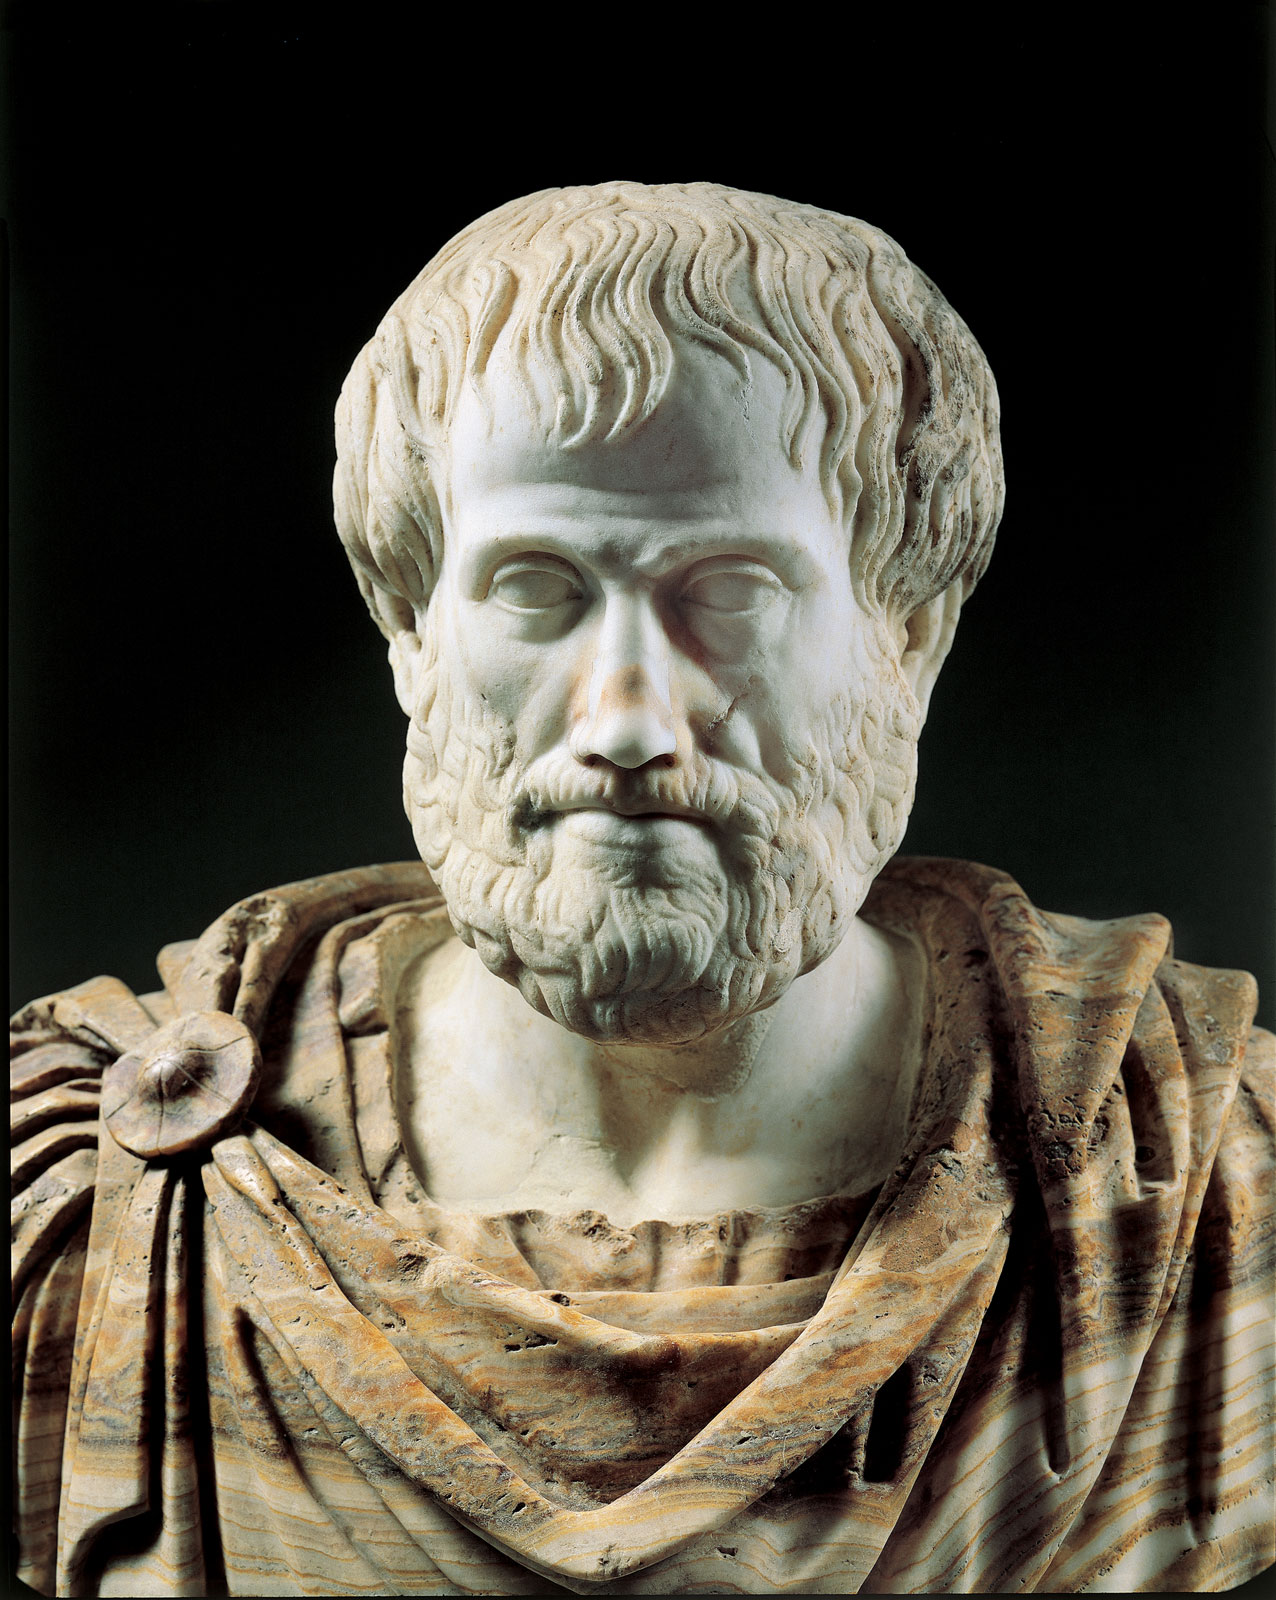
\includegraphics[width=\textwidth]{../assets/aristotle}
    \end{column}
    \begin{column}{.5\textwidth}
      \begin{itemize}
        \item Lived 384--322 BCE
        \item Cataloged valid arguments (``syllogisms''), e.g.,
        \item All ungulates have hooves.\\
        No fish have hooves.\\
        $\therefore$ No fish are ungulates.
      \end{itemize}
    \end{column}
  \end{columns}
\end{frame}

\begin{frame}
  \frametitle{The middle ages}
  \begin{columns}
    \begin{column}{.5\textwidth}
    
\includegraphics[width=\textwidth]{../assets/avicenna}
    \end{column}
    \begin{column}{.5\textwidth}
      \begin{itemize}
        \item Ibn S\=\i n\=a (Avicenna)
        \item Pierre Abelard
        \item William Ockham
        \item Jean Buridan
      \end{itemize}
    \end{column}
  \end{columns}
\end{frame}

\begin{frame}
  \frametitle{Mathematical logic: Boole et al.}

  \begin{columns}
    \begin{column}{.5\textwidth}
    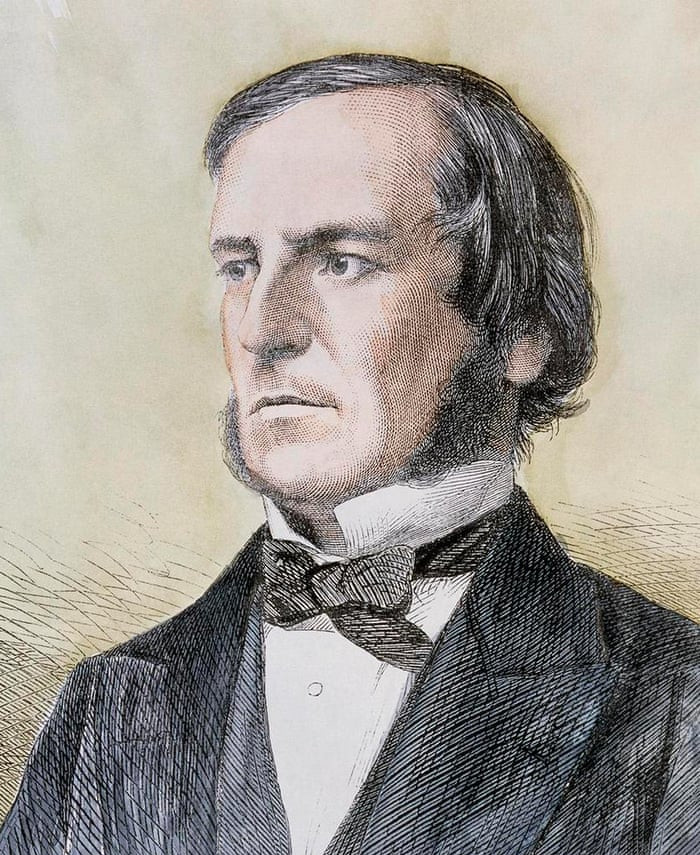
\includegraphics[width=\textwidth]{../assets/boole}
    \end{column}
    \begin{column}{.5\textwidth}
      \begin{itemize}
        \item George Boole
        \item John Venn
        \item Augustus De Morgan
        \item Charles Lutwidge Dodgson (aka Lewis Caroll)
      \end{itemize}
    \end{column}
  \end{columns}
\end{frame}

\begin{frame}
  \frametitle{The algebra of logic: Peirce at al}

  \begin{columns}
    \begin{column}{.5\textwidth}
      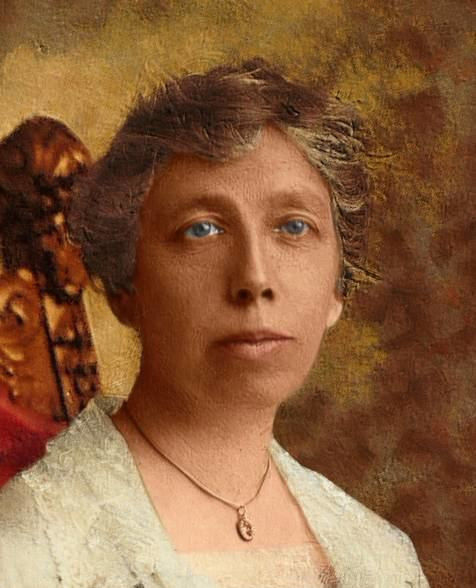
\includegraphics[width=\textwidth]{../assets/ladd-franklin}
    \end{column}
    \begin{column}{.5\textwidth}
      \begin{itemize}
        \item Charles Sanders Peirce
        \item Christine Ladd-Franklin
        \item Ernst Schr\"oder
      \end{itemize}
    \end{column}
  \end{columns}
\end{frame}

\begin{frame}
  \frametitle{Modern logic: Gottlob Frege}

  \begin{columns}
    \begin{column}{.5\textwidth}
      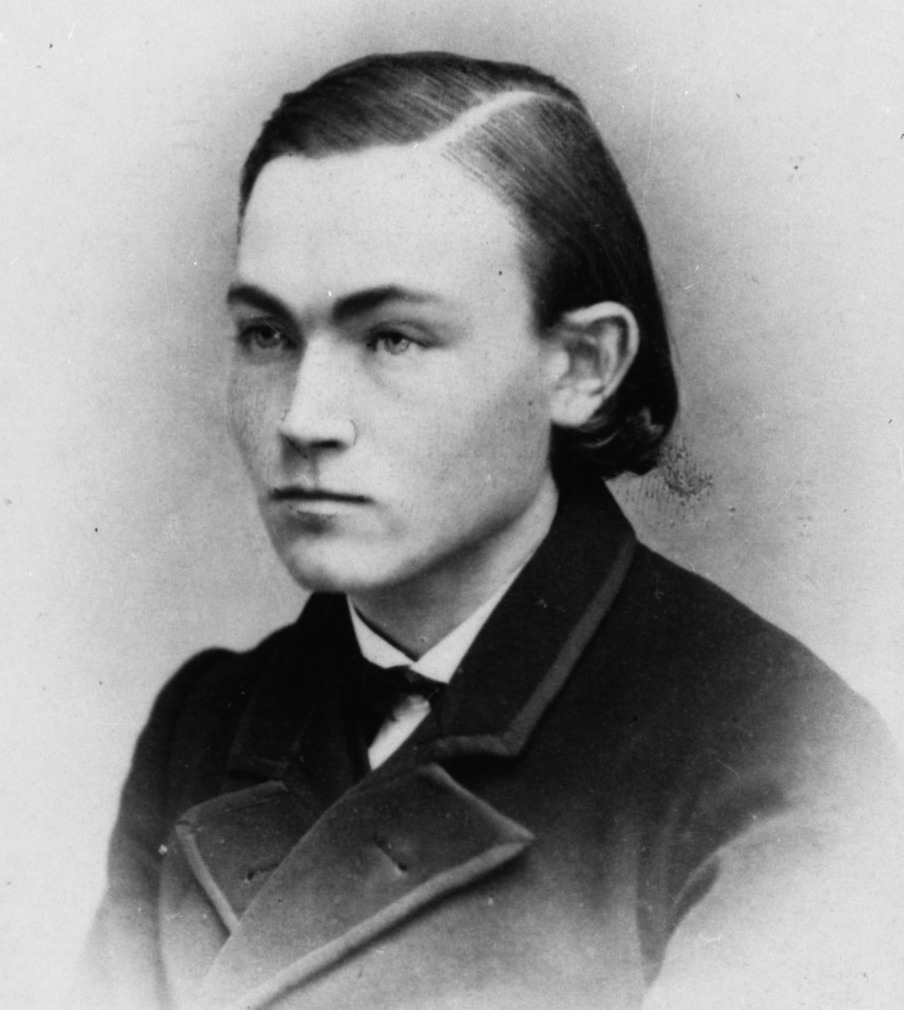
\includegraphics[width=\textwidth]{../assets/frege}
    \end{column}
    \begin{column}{.5\textwidth}
      \begin{itemize}
        \item 1848--1925
        \item Predicates and quantifiers
        \item Plan to turn all of math into theorems of logic alone
      \end{itemize}
    \end{column}
  \end{columns}
\end{frame}

\begin{frame}
  \frametitle{Modern logic: Bertrand Russell}

  \begin{columns}
    \begin{column}{.5\textwidth}
      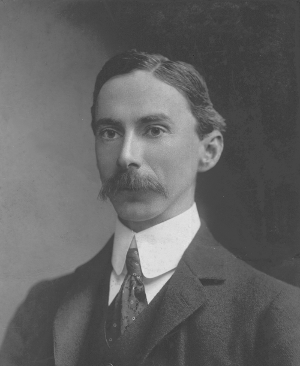
\includegraphics[width=\textwidth]{../assets/russell}
    \end{column}
    \begin{column}{.5\textwidth}
      \begin{itemize}
        \item 1870--1972
        \item Showed Frege's system contradictory
        \item Fixed it (\textit{Principia mathematica}, 3 vols.)
        \item Plan to turn all of math into theorems of logic alone
      \end{itemize}
    \end{column}
  \end{columns}
\end{frame}

\begin{frame}
  \frametitle{Modern logic: David Hilbert}

  \begin{columns}
    \begin{column}{.5\textwidth}
      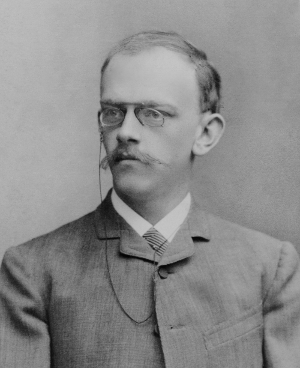
\includegraphics[width=\textwidth]{../assets/hilbert}
    \end{column}
    \begin{column}{.5\textwidth}
      \begin{itemize}
        \item 1862--1943
        \item Combined Russell's and Schr\"oder's systems
        \item First modern logic textbook
        \item Plan to turn all of math into consequences of a single set of premises
      \end{itemize}
    \end{column}
  \end{columns}
\end{frame}

\begin{frame}
  \frametitle{Modern logic: Kurt G\"odel}

  \begin{columns}
    \begin{column}{.5\textwidth}
      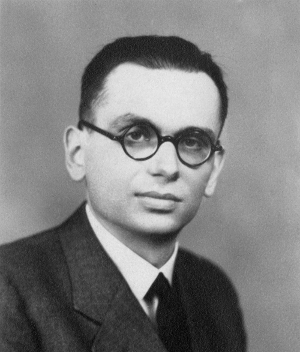
\includegraphics[width=\textwidth]{../assets/goedel}
    \end{column}
    \begin{column}{.5\textwidth}
      \begin{itemize}
        \item 1906--1978
        \item Showed that every valid argument has a proof
        \item Showed that Frege/Russell's and Hilbert's plans can't work
      \end{itemize}
    \end{column}
  \end{columns}
\end{frame}

\begin{frame}
  \frametitle{Modern logic: Alan Turing}

  \begin{columns}
    \begin{column}{.5\textwidth}
      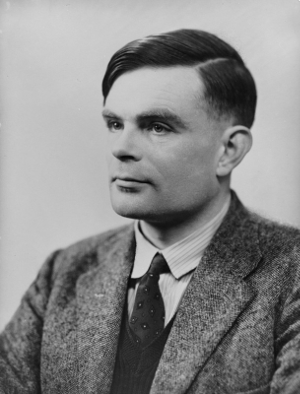
\includegraphics[width=\textwidth]{../assets/turing}
    \end{column}
    \begin{column}{.5\textwidth}
      \begin{itemize}
        \item 1912--1954
        \item Showed that unlike TFL, FOL has no decision procedure
        \item Invented Turing machines (``father of computer science'')
      \end{itemize}
    \end{column}
  \end{columns}
\end{frame}

\begin{frame}
  \frametitle{Modern logic: Gerhard Gentzen}

  \begin{columns}
    \begin{column}{.5\textwidth}
      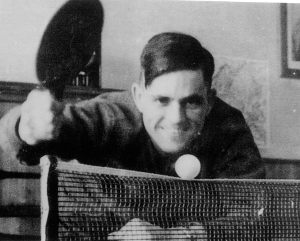
\includegraphics[width=\textwidth]{../assets/gentzen}
    \end{column}
    \begin{column}{.5\textwidth}
      \begin{itemize}
        \item 1909--1945
        \item Invented natural deduction
        \item Founded theory of proofs
      \end{itemize}
    \end{column}
  \end{columns}
\end{frame}

\begin{frame}
  \frametitle{Modern logic: modal logic}

  \begin{columns}
    \begin{column}{.5\textwidth}
      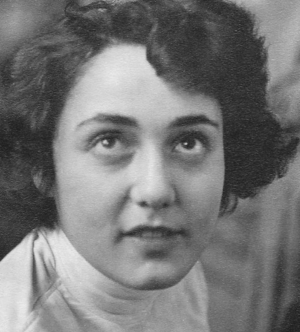
\includegraphics[width=\textwidth]{../assets/barcan}
    \end{column}
    \begin{column}{.5\textwidth}
      \begin{itemize}
        \item Extend logic with operators for ``possible'' and ``necessary''
        \item Pioneered by philosophers, now used by computer scientists
        \item Rudolf Carnap, Saul Kripke, Ruth Barcan Marcus
      \end{itemize}
    \end{column}
  \end{columns}
\end{frame}

\newhourlecture

\subsection{Philosophy and nonstandard logics}

\begin{frame}
    \frametitle{Validity and validity in FOL}

\begin{itemize}[<+->]
\item Philosophers interested in \emph{valid arguments}
\item Definition: There is no case where the
premises are true and the conclusion is false
\begin{itemize}[<+->]
\item \emph{Important:} It does not say ``it \emph{isn't in fact the case} that the premises
are true and the conclusion is false''
\item That would make every argument with
\begin{itemize}
\item true premises, true conclusion
\item false premises, true conclusion
\item false premises, false conclusion
\end{itemize}
valid.  But that's not the case.
\item It says ``it is \emph{impossible} that the premises could be true and the conclusion false!''
\end{itemize}
\item Difficulty: What logically possible circumstances are there?
\end{itemize}

\end{frame}

\begin{frame}
    \frametitle{What logic does for validity}

\begin{itemize}[<+->]
\item Truth-tables, interpretations, proofs give \emph{sufficient conditions}
for validity, i.e.,
\begin{itemize}
\item Every argument valid in TFL is valid
\item Every argument valid in FOL is valid
\item Every argument with a formal proof is valid (soundness!)
\end{itemize}
\end{itemize}

\end{frame}

\begin{frame}
    \frametitle{Nonstandard logics}

\begin{itemize}[<+->]
\item Formal models of logical consequence make a number of simplifying assumptions:
\begin{itemize}[<+->]
\item Only \emph{determinate} properties allowed, e.g, no vague properties
\item Every (atomic) sentence either \True{} or \False; not both and nothing in between
\item Every name must refer, i.e., no empty names
\item Only truth-functional connectives, e.g., no subjunctive contionals, ``because'', or tenses
\end{itemize}
\item Non-standard logics: expand TFL, FOL to deal with these
\end{itemize}

\end{frame}

\begin{frame}
    \frametitle{Many-valued logic}
\def\I{\textcolor{highlightA}{\textbf{U}}}
\begin{itemize}[<+->]
\item Add to the truth-values \True{} and \False, e.g.,
\begin{itemize}
\item ``Undetermined'': neither true nor false
\[
\begin{array}{c|c}
P & \lnot P\\
\hline
\True & \False \\
\I & \I\\
\False & \True
\end{array}
\qquad
\begin{array}{cc|c}
P & Q & (P \land Q)\\
\hline
\True & \True & \True\\
\True & \I & \I\\
\True & \False & \False\\
\I & \True & \I\\
\I & \I & \I\\
\I & \False & \False\\
\False & \True & \False\\
\False & \I & \False\\
\False & \False & \False
\end{array}
\qquad
\begin{array}{cc|c}
P & Q & (P \lor Q)\\
\hline
\True & \True & \True\\
\True & \I & \True\\
\True & \False & \True\\
\I & \True & \True\\
\I & \I & \I\\
\I & \False & \I\\
\False & \True & \True\\
\False & \I & \I\\
\False & \False & \False
\end{array}
\]
\item ``Inconsistent'': both true and false
\item Fuzzy truth values: any number between 0 and 1
\end{itemize}
\end{itemize}

\end{frame}

\subsection{Truth-functionality}

\begin{frame}
\frametitle{Truth-functional connectives}

\begin{block}{Definition}
  A connective $*$ is \emph{truth functional} iff the truth value of $*A$ depends only on the truth value of $A$.
\end{block}

\begin{itemize}[<+->]
  \item ``It is not the case that'' is truth functional.
  \item So are ``and'', ``or'', ``neither nor''.
  \item ``If \dots then'': iffy.
\end{itemize}

\end{frame}


\begin{frame}
  \frametitle{Non-truth-functional connectives}
  
  \begin{itemize}
    \item ``Possibly'', ``Necessarily''
    \item Subjunctive conditionals
    \item Tenses: ``Is always true,'' ``Will be true,'' ``Was true''
    \item ``Richard believes that'', ``Richard knows that''
  \end{itemize}
  \end{frame}
  
\begin{frame}
\frametitle{Possibly}

  \begin{itemize}[<+->]
    \item ``It is possible that \dots'', ``Possibly, \dots''
    \item Consider:
      \begin{enumerate}[<+->]
        \item It is possible that I will live forever.
        \item It is possible that $2+2=5$.
      \end{enumerate}
    \item (1) is true and (2) is false.
    \item But $A_1=$ ``I will live forever'' and
    $A_2=$ ``$2+2=5$'' are both false.
    \item So ``It is possible that $A$'' can't just depend on the
    truth value of $A$
    \item Otherwise (1) and (2) would have to have the same truth value.
  \end{itemize}

\end{frame}

\begin{frame}
\frametitle{Subjunctive Conditionals}

\begin{itemize}[<+->]
\item Subjunctive conditionals = if---then statements in \emph{subjunctive} mood
\item ``If P were true, then Q would be true.''
\item Indicative conditional is (plausibly) \emph{truth-functional}:
  truth value of ``If P, then Q'' depends \emph{only on truth values}
  of P and Q.
\end{itemize}
\end{frame}

\begin{frame}
\frametitle{Subjunctive Conditionals}

\begin{itemize}[<+->]
\item Subjunctive conditional is not truth functional
\item E.g., consider:
\begin{enumerate}
\item If the world were just, no evil deed would go unpunished.\\
$P_1$ = the world is just\\
$Q_1$ = no evil deed goes unpunished
\item If the world were flat, no evil deed would go unpunished.\\
$P_2$ = the world is flat\\
$Q_2$ = no evil deed goes unpunished
\end{enumerate}
\item $P_1$, $Q_1$ both false; $P_2$, $Q_2$ both false, but
\item (1) is true, but (2) is false
\end{itemize}
\end{frame}

\begin{frame}
    \frametitle{Modal logic}

\begin{itemize}[<+->]
\item Alethic logic\\
``It is possible that'' ($\Diamond$), ``it is necessary that'' ($\Box$)
\[
\Box A \to A \qquad \Diamond\Box A \to \Box A
\]
\item Epistemic logic:
``Richard knows that'' (K)
\[
\textbf{K}\, A \to A \qquad \textbf{K}\,\lnot \textbf{K}\, A \to \lnot \textbf{K}\, A
\]
\item Conditional logic\\
Subjunctive conditionals, ``if it were true that \dots, then it would be true that --- ---'' ($\Box\!\!\to$)
\[
(A \mathrel{\Box\!\!\to} B) \to (A \to B)
\]
\item Temporal logic\\
``It was true that'' (P), ``It will be true that'' (F)
\[
\textbf{F}\,\textbf{P}\, A \to (\textbf{P}\, A \lor A \lor \textbf{F}\, A)
\]
\end{itemize}

\end{frame}

\begin{frame}
\frametitle{Temporal logic}

\begin{itemize}[<+->]
  \item ``Always $A$'': $\Box A$
  \item ``Sometimes $A$'': $\Diamond A$
  \item If always $A$, then $A$ (now): $\Box A \to A$
  \item If $A$ (now), then sometimes $A$: $A \to \Diamond A$
  \item Always $A$ iff not sometimes not~$A$\\
  $\Box A \eiff \enot\Diamond \enot A$.
  \item If always $A$ and $B$, then always $A$ or always $B$:\\
  $\Box(A \land B) \eif (\Box A \land \Box B)$
  \item If always $A$ or $B$, then always $A$ or always $B$:
  $\Box(A \lor B) \eif (\Box A \lor \Box B)$
\end{itemize}
\end{frame}

\begin{frame}
\frametitle{Semantics for TFL}

\begin{itemize}[<+->]
  \item Recall: valuations map sentence letters to truth values
  \item Given a valuation $v$, we can define if a sentence of TFL is
  true on~$v$:
  \begin{itemize}
    \item $v \models P$ iff $v(P) = \True$
    \item $v \models \lnot \metav{A}$ iff not $v \models \metav{A}$
    \item $v \models (\metav{A} \lor \metav{B})$ iff $v \models
    \metav{A}$ or $v \models \metav{B}$.
    \item $v \models (\metav{A} \land \metav{B})$ iff $v \models
    \metav{A}$ and $v \models \metav{B}$.
    \item $v \models (\metav{A} \eif \metav{B})$ iff either not $v
    \models \metav{A}$ or $v \models \metav{B}$.
  \end{itemize}
\end{itemize}
\end{frame}

\begin{frame}
\frametitle{Semantics for temporal logic}

\begin{itemize}[<+->]
  \item Collection of points in time $t$
  \item For every time $t$, a valuation $v_t$
  \item Define $\metav{A}$ is true \emph{at time~$t$}:
  \begin{itemize}
    \item $t \models P$ iff $v_t(P) = \True$
    \item $t \models \lnot \metav{A}$ iff not $t \models \metav{A}$
    \item $t \models (\metav{A} \lor \metav{B})$ iff $t \models
    \metav{A}$ or $t \models \metav{B}$.
    \item $t \models (\metav{A} \land \metav{B})$ iff $t \models
    \metav{A}$ and $t \models \metav{B}$.
    \item $t \models (\metav{A} \eif \metav{B})$ iff either not $t
    \models \metav{A}$ or $t \models \metav{B}$.
    \item $t \models \alert{\Box \metav{A}}$ iff, at \alert{all times $s$}, $\alert{s} \models \metav{A}$
    \item $t \models \alert{\Diamond \metav{A}}$ iff, at \alert{some time $s$}, $\alert{s} \models \metav{A}$
  \end{itemize}
\end{itemize}
\end{frame}

\begin{frame}
  \frametitle{Validity}

  \begin{itemize}[<+->]
    \item Some sentences are always true, however we interpret sentence letters, e.g.,
    \[ \Box A \eif \lnot\Diamond\lnot A\]
    \item Suppose at time $t$, $t \models \Box A$.
    \item Then at all times $s$, $s \models A$.
    \item So at no time $s$, $s \models \lnot A$.
    \item So not: at some time $s$, $s \models \lnot A$.
    \item So not: $t \models \Diamond\lnot A$.
    \item Therefore: $t \models \lnot\Diamond\lnot A$.
  \end{itemize}
\end{frame}

\begin{frame}
  \frametitle{Invalidity}

\begin{itemize}[<+->]
  \item Some sentences are not always true
  \item Obviously, any sentence not involving $\Box$, $\Diamond$ that
  isn't a tautology
  \item But also, e.g., $\Box(A \lor B) \eif (\Box A \lor \Box B)$
  \item Counterexample:
  \begin{itemize}
    \item Two times, $1$ and $2$.
    \item $v_1(A) = v_2(B) = \True$, $v_2(A) = v_2(B) = \False$
    \item $1 \models A \lor B$ (since $1 \models A$)
    \item $2 \models A \lor B$ (since $2 \models B$)
    \item So at every time $t$, $t \models A \lor B$
    \item So $1 \models \Box(A \lor B)$
    \item But neither $1 \models \Box A$ nor $1 \models \Box B$
  \end{itemize}
\end{itemize}
\end{frame}

% phil279 lec 21 has soundness & completeness


\newhourlecture

\subsection{Semantics and proof theory}

\begin{frame}
    \frametitle{Semantics}

\begin{itemize}
\item A \emph{truth-value assignment} is an assignment of \True{} or \False{} to the sentence letters (schematic letters in the truth-functional form)
\item An \emph{interpretation} is a non-empty domain together with
\begin{itemize}
\item extensions for each predicate symbol
\item objects in the domain for each constant symbol
\item functions for each function symbol
\end{itemize}
\item A tautology is a sentence (the truth-functional form of) which is true in all truth-value assignments
\item A validity is a sentence that's true in all interpretations
\end{itemize}
\end{frame}


\begin{frame}
    \frametitle{Soundness and completeness}

\begin{itemize}[<+->]
\item Soundness

Arguments have formal proofs only if they are valid\\
If there is a proof of $B$ from premises $ A_1, \dots A_n$, then $B$ is a consequence of $ A_1, \dots A_n$

\item Completeness

Arguments have formal proofs if they are valid\\
If $ A_1, \dots A_n$ entail $B$ in FOL, then there is a proof of $B$ from premises $ A_1, \dots A_n$\\[2ex]
Proved by Kurt G\"odel (1929)
\end{itemize}
\end{frame}

\begin{frame}
    \frametitle{Other proof systems: resolution}

    \begin{itemize}
\item Natural deduction is a proof system for \emph{validity/tautologies}
\item Also possible to design proof systems for dual notion: \emph{unsatisfiability}\\
($A$ is a tautology $\Leftrightarrow$ $\lnot A$ is unsatisfiable)
\item A \emph{clause} is a disjunction $ A_1 \lor \ldots \lor A_n$
where each $ A_i$ is atomic or negated atomic.
\item CNF theorem: every sentence is equivalent to a conjunction of clauses.
\end{itemize}
\end{frame}

\begin{frame}
  \frametitle{Other proof systems: resolution}

  \begin{itemize}
\item The resolution rule:
\begin{fitchproof}
\hypo[ ]{1}{A_1 \lor \ldots \lor A_n \lor C}
\hypo[ ]{2}{B_1 \lor \ldots \lor B_m \lor \lnot C}
\have[ ]{3}{A_1 \lor \ldots \lor A_n \lor B_1 \lor \ldots \lor B_m}
\end{fitchproof}
\item Preserves \emph{joint satisfiability}
\item If you can prove the empty clause $\bot$ from a set of clauses, they can't be
jointly satisfiable.
\end{itemize}
\end{frame}

\subsection{Theories and decidability}

\begin{frame}
    \frametitle{Church-Turing Theorem}

\begin{block}{Instance: Sentence $A$ of FOL\\
Problem: Is $A$ a validity?}

\begin{itemize}
\item Undecidable: no computer program can answer this question correctly for all $A$.
\item Proved independently by Alonzo Church and Alan Turing in 1935
\end{itemize}
\end{block}
\end{frame}


\begin{frame}
  \frametitle{Cook's Theorem}

\begin{block}{Instance: Sentence $A$ of TFL\\
Problem: Is $A$ a tautology?}

\begin{itemize}
\item Decidable: write a computer program that checks all valuation for $A$.
\item But: it's hard: ``co-NP complete''
\item Proved independently by Stephen Cook (1971) and Leonid Levin (1973)
\end{itemize}
\end{block}
\end{frame}


\begin{frame}
    \frametitle{Decidable Classes}

\begin{itemize}
\item The decision problem \emph{in general} is undecidable
\item But special cases \emph{can} be decided, e.g.:
\end{itemize}
\begin{block}{Instance: Sentence $A$ with only 1-place predicate symbols\\
Problem: Is $A$ a validity?}

\begin{itemize}
\item Decidable
\item Proved by Leopold L\"owenheim (1915)
\item Complexity is NEXPTIME-complete.
\end{itemize}
\end{block}
\end{frame}

\begin{frame}
    \frametitle{Theories}

\begin{itemize}
\item A set of sentences of FOL also called a \emph{theory}, and the sentences in it \emph{axioms}
\item Some (types of) interpretations can be characterized
as those interpretations in which every sentence in the theory is true
\item Examples:
\begin{itemize}
\item Mathematical theories (theory of orders, group theory, arithmetic)
\item KR classification systems, e.g., SNOMED-CT
\item Mereology, theories of truth, scientific theories
\end{itemize}
\end{itemize}
\end{frame}

\begin{frame}
    \frametitle{The axiomatic method}

\begin{itemize}
\item Theories + logic: what follows from axioms?
\item Axiomatic method: do science by investigating what follows from
  the axioms of a theory
\item Logic can also determine:
\begin{itemize}
\item Are axioms (in)consistent?
\item Are axioms independent, or is one superfluous?
\end{itemize}
\item Paradigm of axiomatic method: geometry (Euclid)
\end{itemize}
\end{frame}

\begin{frame}
    \frametitle{Examples of theories: linear orders}

A relation $\preceq$ on a set $O$ is a \emph{linear order} iff
it makes following axioms true:
\begin{align*}
& \forall x\forall y((x \preceq y \land y \preceq x) \to x = y) & \text{Antisymmetry}\\
& \forall x\forall y\forall z((x \preceq y \land y \preceq z) \to x \preceq z) &\text{Transitivity}\\
& \forall x\forall y(x \preceq y \lor y \preceq x) & \text{Totality}
\end{align*}
Every total relation is reflexive:
\[
{ LO} \models \forall x\, x \preceq x
\]
\end{frame}

\begin{frame}
    \frametitle{Examples of theories: Robinson's Q}

Theories of arithmetic, such as Robinson's theory Q:
\begin{align*}
 \lnot\exists x\, (x + 1) & = 0\\
 \forall x(x = 0  \lor \exists y\, (y+1) & = x)\\
 \forall x\forall y((x + 1) = (y + 1)  \to x & = y)\\
 \forall x\,(x + 0) & = x\\
 \forall x\forall y\, (x + (y+1)) & = ((x + y) +1) \\
 \forall x\,(x \times 0) & = 0\\
 \forall x\forall y\, (x \times (y + 1)) & = ((x \times y) + x)
\end{align*}
\end{frame}



\begin{frame}
    \frametitle{Examples of theories: SNOMED-CT}

\begin{align*}
\texttt{bacterial } & \texttt{pneumonia} = \\
& \texttt{is-a|bacterial infectious disease}\\
& \texttt{is-a|infective pneumonia}\\
& \texttt{causative agent|bacteria}\\
& \texttt{finding site|lung structure}
\end{align*}
\begin{align*}
\forall x(& BacterialPneumonia(x) \eiff  \\
& BacterialInfectiousDisease(x) \land\\
& InfectivePneumonia(x) \land \\
& \exists y(HasCausativeAgent(x, y) \land Bacteria(y)) \land\\
&\exists y(HasFindingSite(x, y) \land LungStructure(y)))
\end{align*}
\end{frame}

\begin{frame}
    \frametitle{Examples of theories: SNOMED-CT}

\begin{itemize}
\item Over 300,000 concepts (predicate symbols), e.g.,\\
\begin{itemize}
\item 1-place predicates:\\
parts of body, findings, organisms, physical objects, procedures, substances, diseases, \dots
\item 2-place predicates:\\
has finding site, has causative agent, with method, has active ingredient, laterality is, using device, \dots
\end{itemize}
\item About 1,000,000 descriptions (axioms)
\item SNOMED-CT is decidable
\end{itemize}

\end{frame}

\begin{frame}
    \frametitle{Examples of Theories: Mereology}

\begin{itemize}
\item Mereology: the theory of the part-whole relation (\emph{metaphysics})
\item Primitive relation: $Pt(x, y)$, ``$x$ is a part of $y$''
\item Some axioms:
\begin{align*}
& \forall x\, Pt(x, x) & \text{Reflexivity}\\
& \forall x\forall y\forall z((Pt(x,y) \land Pt(y, z)) \to Pt(x,z)) & \text{Transitivity}\\
& \forall x\forall y((Pt(x, y) \land Pt(y, x)) \to x = y) & \text{Antisymmetry}
\end{align*}
\end{itemize}
\end{frame}

\begin{frame}
  \frametitle{Examples of Theories: Mereology}

\begin{itemize}
\item Defined properties and relations
\begin{align*}
PP(x, y) & \eiff Pt(x, y) \land \lnot x = y \\
At(x) & \eiff \lnot\exists y\,PP(y, x)
\end{align*}
\item Different theories settle questions differently, e.g.,
\begin{itemize}
\item Are there atoms?
\item Does everything comprise at least one atom?
\item Is everything made of atomless ``gunk''?
\end{itemize}
\end{itemize}

\end{frame}

\begin{frame}
    \frametitle{Property theories and Grelling's paradox}

\begin{itemize}
\item Primitive relation: $Ap(x ,y)$, ``$x$ applies to $y$''
\item Proposed axiom (``comprehension''): For any formula $P(y)$,
\[
\exists x\forall y(Ap(x, y) \eiff P(y))
\]
\item Axiom is \emph{inconsistent} (contradictory)
\item A property is \emph{heterological} if it does not apply to itself, i.e., $
 \lnot Ap(x, x)$
\item Is the property of being heterological itself heterological?
\end{itemize}
\begin{fitchproof}
\hypo[ ]{1}{\forall y(Ap(h, y) \eiff \lnot Ap(y, y))}
\have[ ]{2}{Ap(h, h) \land \lnot Ap(h, h)}
\end{fitchproof}
\end{frame}

\begin{frame}
    \frametitle{Completeness of theories}

\begin{itemize}
\item A theory T is \emph{complete} if for every sentence $A$ in its language,
either $ T \models A$ or $ T \models \lnot A$
\item Every complete theory is decidable!
\item Some incomplete theories are still decidable (e.g., $LO$)
\item Some incomplete theories are incomplete\emph{able}: no consistent extension is complete
\item Philosophical upshot of this: truth in the intended interpretation(s) of the theory outstrips provability from the theory
\end{itemize}
\textbf{G\"odel's Incompleteness Theorem (1930)}\\
Arithmetic, set theory, mereology are incompleteable

\end{frame}


\subsection{A logical party trick}


\begin{frame}
\frametitle{Easter bunny party trick}
\small
If the first sentence on this slide is true, \\\qquad then the Easter Bunny exists.

\begin{enumerate}[<+->]
\item Assumption: The first sentence on this slide is true.
\item If the first sentence on this slide is true, then  the Easter Bunny exists (from (1), since if $S$ is true, then $S$).
\item The Easter Bunny exists \\\qquad(from (1) and (2), by modus ponens)
\item If the first sentence on this slide is true,  the Easter Bunny exists\\\qquad(from (1)--(3), by conditional intro).
\item The first sentence on this slide is true.\\\qquad ((4) = the first sentence on this slide)
\item The Easter Bunny exists.\\\qquad (from (4) and (5), by modus ponens)
\end{enumerate}
\end{frame}

\end{document}